\documentclass[a4paper]{article}

%% Language and font encodings
\usepackage[english]{babel}
\usepackage[utf8x]{inputenc}
\usepackage[T1]{fontenc}
\usepackage{booktabs}
\usepackage{multirow}
\usepackage{lineno}

%% Sets page size and margins
\usepackage[a4paper,top=3cm,bottom=2cm,left=3cm,right=3cm,marginparwidth=1.75cm]{geometry}

%% Useful packages
\usepackage{amsmath}
\usepackage{graphicx}
\usepackage[colorinlistoftodos]{todonotes}
\usepackage[colorlinks=true, allcolors=blue]{hyperref}
\usepackage{siunitx}
% \usepackage{subfigure}
\usepackage{subcaption}


\graphicspath{{_fig_optical/}}
\linenumbers

\title{Electron-neutrino reconstruction in MicroBooNE using the Pandora reconstruction framework}
\author{The MicroBooNE collaboration}

\begin{document}
\maketitle
\tableofcontents

\listoftodos

\begin{abstract}
MicroBooNE (the Micro Booster Neutrino Experiment) is a liquid argon
time-projection chamber experiment designed for short-baseline neutrino physics, currently running at Fermilab. It aims to address the anomalous excess of low-energy events observed by the previous MiniBooNE experiment. In this note we demonstrate the ability of the experiment to reconstruct electron neutrino-like events in the detector, using the Pandora reconstruction framework. In particular, we present a fully automated event selection algorithm that can identify charged-current electron neutrino event candidates with no pions and at least one proton in the final state.
\end{abstract}


\section{Introduction}
One of the main physics goals of the MicroBooNE experiment is to clarify the nature of the low-energy excess of $\nu_{e}$-like events observed by the MiniBooNE experiment in 2009. The excess was found in the neutrino energy region between 200 to 475 MeV in 2009.

However, the MiniBooNE detector was a \v{C}erenkov detector, which is not able to distinguish between single electrons and single photons in the final state, making it impossible to pick a physics model among those which could explain the excess.

The MicroBooNE detector, instead, is a liquid argon time projection chamber. This technology provides detailed tracking and allows to measure the rate of energy loss per length of each particle ($dE/dx$), which is essential for electron/photon identification.

In this note we will describe an algorithm which aims to select $\nu_{e}$ interactions in the MicroBooNE detector in a $\nu_{\mu}$ beam, such as the Booster Neutrino Beam (BNB) at the Fermi National Accelerator Laboratory.

% In this section, highlight the following:
% Why are we picking to do 1eNp?
% - Similar to Miniboone, in that this focuses on events from a predominantly CCQE interaction
% - Addition of vertex activity (Np) allows more aggressive cosmic rejection, and improves vertex tagging in Pandora
% - Requirement of only protons at the vertex reduces statistics, but allows for a track-length based calorimetry of protons which improves resolution.

\section{Signal definition}
The Standard Model, at tree level, allows only weak interaction for neutrinos. As such, neutrinos exchange a $W^{\pm}$ vector boson in charged-current (CC) interactions and a $Z$ vector boson in neutral-current (NC) interactions. 
However, the energy of a neutrino can range from few keV to several PeV, as recently measured by the IceCube experiment \cite{icecube}, producing wildly different topologies in the final state. 
In our case, we are interested in $\nu_{e}$ CC interactions in the sub-GeV region (0.1 - 1~GeV). In a naive scenario, where we ignore nuclear and final-state interactions, we can have three dominant outcomes:
\begin{itemize}
\item Charged Current Quasi Elastic (CCQE): it is the principal signature for most neutrino experiments. The neutrino exchanges a $W^{\pm}$ with a neutron, producing a proton and a charged lepton in the final state.
\item Charged Current Resonant production (CCRES): the neutrino excites a nucleon, which emits a pion.
\item Charged Current Deep Inelastic Scattering (CCDIS): the neutrino interacts with a quark, producing a shower of particles as the nucleus breaks apart.
\end{itemize}

However, hadrons exiting the nucleus after the neutrino interaction can re-interact and change identity or eject other hadrons (Final State Interactions, FSI) \cite{ccqe2}. It is then necessary to define the signal by the particles in its final state. Our selection aims to have a sample with one electron, no other leptons or photons, at least one proton, and no other hadrons or mesons. This kind of event is called CC0$\pi$-Np (where N > 0) \cite{teppei}.

In a LArTPC, the final state of a contained $\nu_{e}$ CC0$\pi$-Np interaction will correspond in general to one or more ionisation tracks, produced by the protons, and an electromagnetic shower, produced by the electron. A charged pion in the final state, instead, will decay mainly into a muon, producing a second ionisation track, while a neutral pion will decay into two photons, producing two electromagnetic showers. 
CCDIS interactions, whose branching ratio is relatively small in the sub-Gev region, usually produce large hadronic jets, which are reconstructed as a combination of tracks and showers. 

%As such, a perfect reconstruction of a $\nu_{e}$ CCQE-like event in a LArTPC will produce as many ionisation tracks as the number of protons in the final state and a single electromagnetic shower (the electron), sharing a common vertex.

The MiniBooNE experiment showed an excess of CCQE-like events (one proton and one electron in the final state) in the 200-475~MeV neutrino energy range \cite{miniboone}, so our analysis will focus on a similar topology in an analogous energy range.
% This section describes the methodology of the selection
% The following sections should be here:
% - Optical Precuts
% - Optical Flash Matching
% - Cosmic Hit Removal and NuMu removal (reference marco only, really)
% - Preselection with 1+tracks, 1+showers OR 2+ showers
% - Pion and Muon Rejection in tracks (AKA, proton selection)
% - Background Rejection Cuts

\section{Analysis Methodology}
\label{sec:methodology}

% This section will describe the methodology used in this analysis, and the details of some of the technical aspects of the methodology (optical flash matching, dE/dx calculation, proton PID, etc).  Some of the cuts of the analysis that are well developed and static are described in this section, for example the optical precuts.  Other cuts, such as the background rejection cuts applied after the preselections, are described in Section~\ref{sec:electron_like} though the techniques used to calculated these variables are described here.

In the TPC, ionisation electrons passing through the MicroBooNE cryostat are drifted to the anode, inducing electric signals on the wires of the three TPC planes. The waveforms observed for each wire are examined and a hit-finding algorithm searches for local maxima and minima. A Gaussian distribution is fitted to each peak and hit objects are created. The hits are used by the reconstruction algorithms provided by the Pandora framework \cite{pandora} to form TPC reconstructed objects. 

The Pandora reconstruction produces as a first stage a list of two-dimensional clusters, which represent continuous, unambiguous lines of hits. Then, cluster-merging algorithms identify associations between multiple clusters. The three-dimensional track and shower reconstruction then collects the two-dimensional clusters from the three readout planes that represent individual track-like or shower-like objects \cite{pandora2}. Our analysis relies on these high-level reconstructed objects to select our CC0$\pi$-Np candidates.

MicroBooNE is also equipped with an optical system made of 32 photomultipliers tubes placed behind the anode plane, with few-ns timing resolution. The optical system detects the argon scintillation light produced by the neutrino interaction and it provides the TPC start time of the event.
Figure \ref{fig:evd} shows a simulated event display of one wire plane with an electron and two protons in the final state, with the corresponding reconstructed shower and reconstructed tracks. In this case, the algorithm was able to correctly reconstruct the electromagnetic shower and both proton tracks.

\begin{figure}[htbp]
	\begin{center}
    	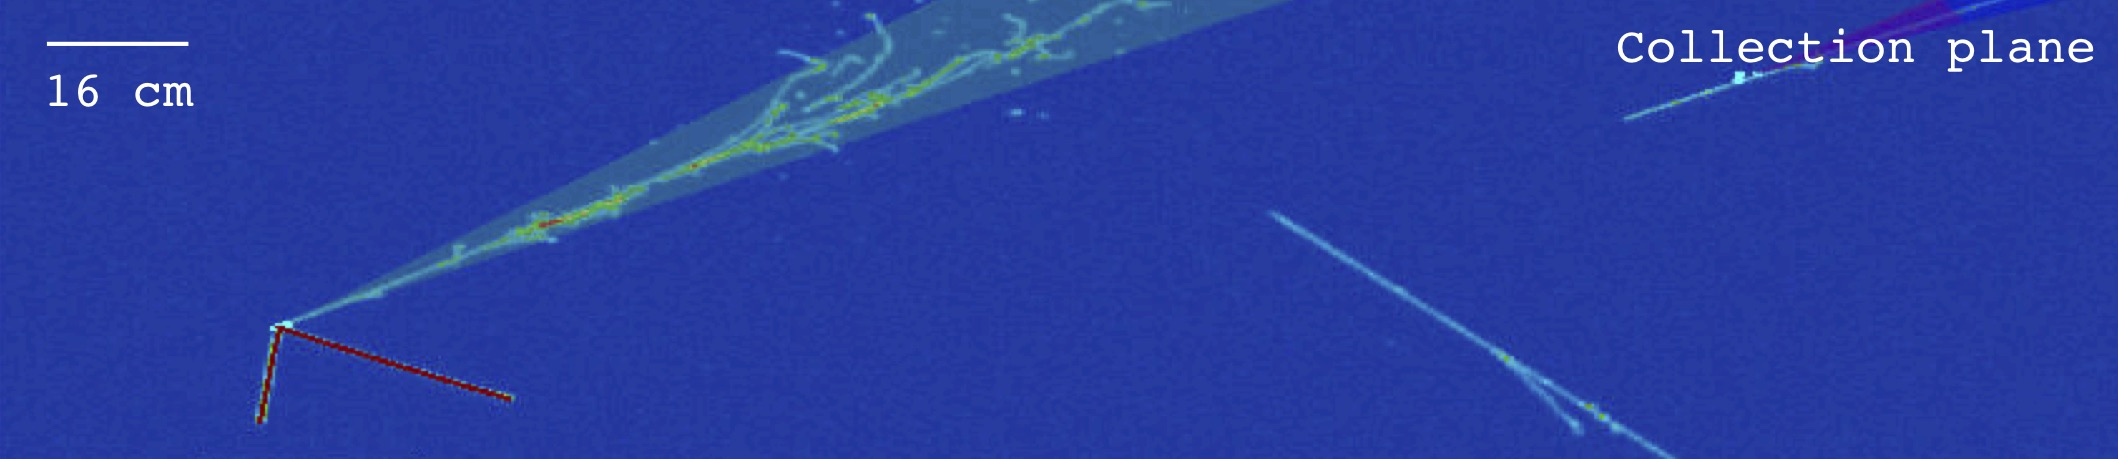
\includegraphics[width=0.8\linewidth]{figures/evd.jpg}
    	\caption{Monte Carlo event display of the collection plane with an electron and two protons in the final state. The reconstructed shower-like object is represented by the green cone. The reconstructed track-like objects are represented by the red lines.} \label{fig:evd}
	\end{center}
\end{figure}

% Our $\nu_{e}$ CC0$\pi$-Np selection algorithm first looks for (1) a flash in the optical system compatible with one of the neutrino interaction candidates provided by the Pandora framework, plus (2) a neutrino interaction candidate with one or more track-like objects and one or more shower-like objects, or two or more shower-like objects. 
% Then, the $\nu_{\mu}$ and cosmic-ray candidates selected by an external module \cite{ubxsec} are removed from the sample. The signal events  Finally, the energy spectrum of the $\nu_{e}$ CC0$\pi$-Np candidates is measured with the procedure described in Section \ref{sec:energyreco}.

\subsection{Overview}

The reconstruction and selection of electron neutrino candidate events for this analysis has been divided into several stages:
\begin{enumerate}
\item Optical pre-cuts and flash-matching: a minimum amount of photoelectrons in the optical system is required. At least one of the neutrino candidates provided by the Pandora framework must be then compatible with the flash in the optical system.
\item Electron neutrino topological pre-selection: one of the neutrino candidates must be compatible with the topology of a $\nu_{e}$ CC0$\pi$-Np interaction, that is at least one track and at least one shower or at least two showers sharing a common vertex.  Multiple showers are accepted due to track/shower mis-identification, discussed later.
\item CC $\nu_{\mu}$ neutrino and cosmic-ray candidates removal: events tagged as CC $\nu_{\mu}$ neutrino candidates or non-neutrino induced are vetoed by an external module.
\item Background rejection through calorimetric and geometric cuts: $\nu_{e}$ CC0$\pi$-Np events are further isolated applying several boxed cuts on kinematic, geometric, and calorimetric variables. The electromagnetic showers initiated by an electron in the final state are isolated with a cut on the $dE/dx$ value. The proton tracks are selected with a Boosted Decision Tree trained on the track $dQ/dx$ and its length.
\item Energy spectrum reconstruction: the energy of the electron showers is measured with a hit-based procedure, while the energy deposited by the proton tracks is calculated from the length of the reconstructed track. 
\end{enumerate}

\subsection{Cosmic Hit Removal}
As a surface experiment, the MicroBooNE detector is constantly hit by atmospheric cosmic rays, at a rate of $\sim 5$~kHz \cite{cosmic}. These cosmic rays will interact in the TPC, producing a combination of track-like and shower-like objects. 
In order to suppress this cosmogenic background, the Pandora framework runs in two different modes with different settings \cite{pandora}: (1) \texttt{pandoraCosmic}, optimized for cosmic rays reconstruction, and (2) \texttt{pandoraNu}, optimized for neutrino interactions reconstruction.
The reconstructed hits are first fed to the framework in the \texttt{pandoraCosmic} mode. Then, a series of cosmic-ray tagging algorithms are applied to the objects reconstructed by Pandora in this mode \cite{ubxsec}. The reconstructed hits that are deemed to be of cosmic origin by the tagging algorithms are removed from the hit collection. The remaining hits are then fed again to the framework in the \texttt{pandoraNu} mode, which reconstructs the neutrino interaction candidates.

\subsection{Optical Pre-Cuts}\label{sec:optical_pre_cuts}
The optical selection requirements serve two purposes beyond a simple trigger condition.  First, they ensure that the optical flash that triggered the detector readout is compatible with the neutrino candidates from the \texttt{pandoraNu} reconstruction pass.  Second, they provide a way to discriminate between multiple \texttt{pandoraNu} neutrino candidate objects (most of which are cosmics) by selecting the one most compatible with the in-time flash.

The first requirement ensures the presence of light in the detector in a position compatible with the center of the collected charge of the neutrino interaction candidate and with a timing compatible with the beam-gate window.

It is also possible and likely that an event will have multiple neutrino candidates. The goal of the optical selection is reducing the number of candidates to maximal one candidate in each event. This process consists of three major parts:
\begin{enumerate}
\item Rectangular cuts are applied to optical properties of the reconstructed flash object.
\item Rectangular cuts on the compatibility of the reconstructed flash with the Pandora neutrino candidate.
\item The Pandora neutrino candidate which is most compatible with the flash is picked using a likelihood method.
\end{enumerate}

To demonstrate the effect of the used cuts, they will be applied on two different samples, both of which were produced with Monte Carlo Challenge 8.3:
\begin{itemize}
\item The signal sample: BNB $\nu_e$ intrinsic with cosmic rays
\begin{itemize}
\item The truth vertex should be in the fiducial volume.
\item There should be an electron with a kinetic energy of at least \SI{20}{\MeV}.
\item There should be at least one proton wit a kinetic energy of \SI{40}{\MeV} or higher.
\end{itemize}
\item The background sample: CORSIKA in-time cosmic rays
\end{itemize}

\begin{figure}[!htbp]
\centering
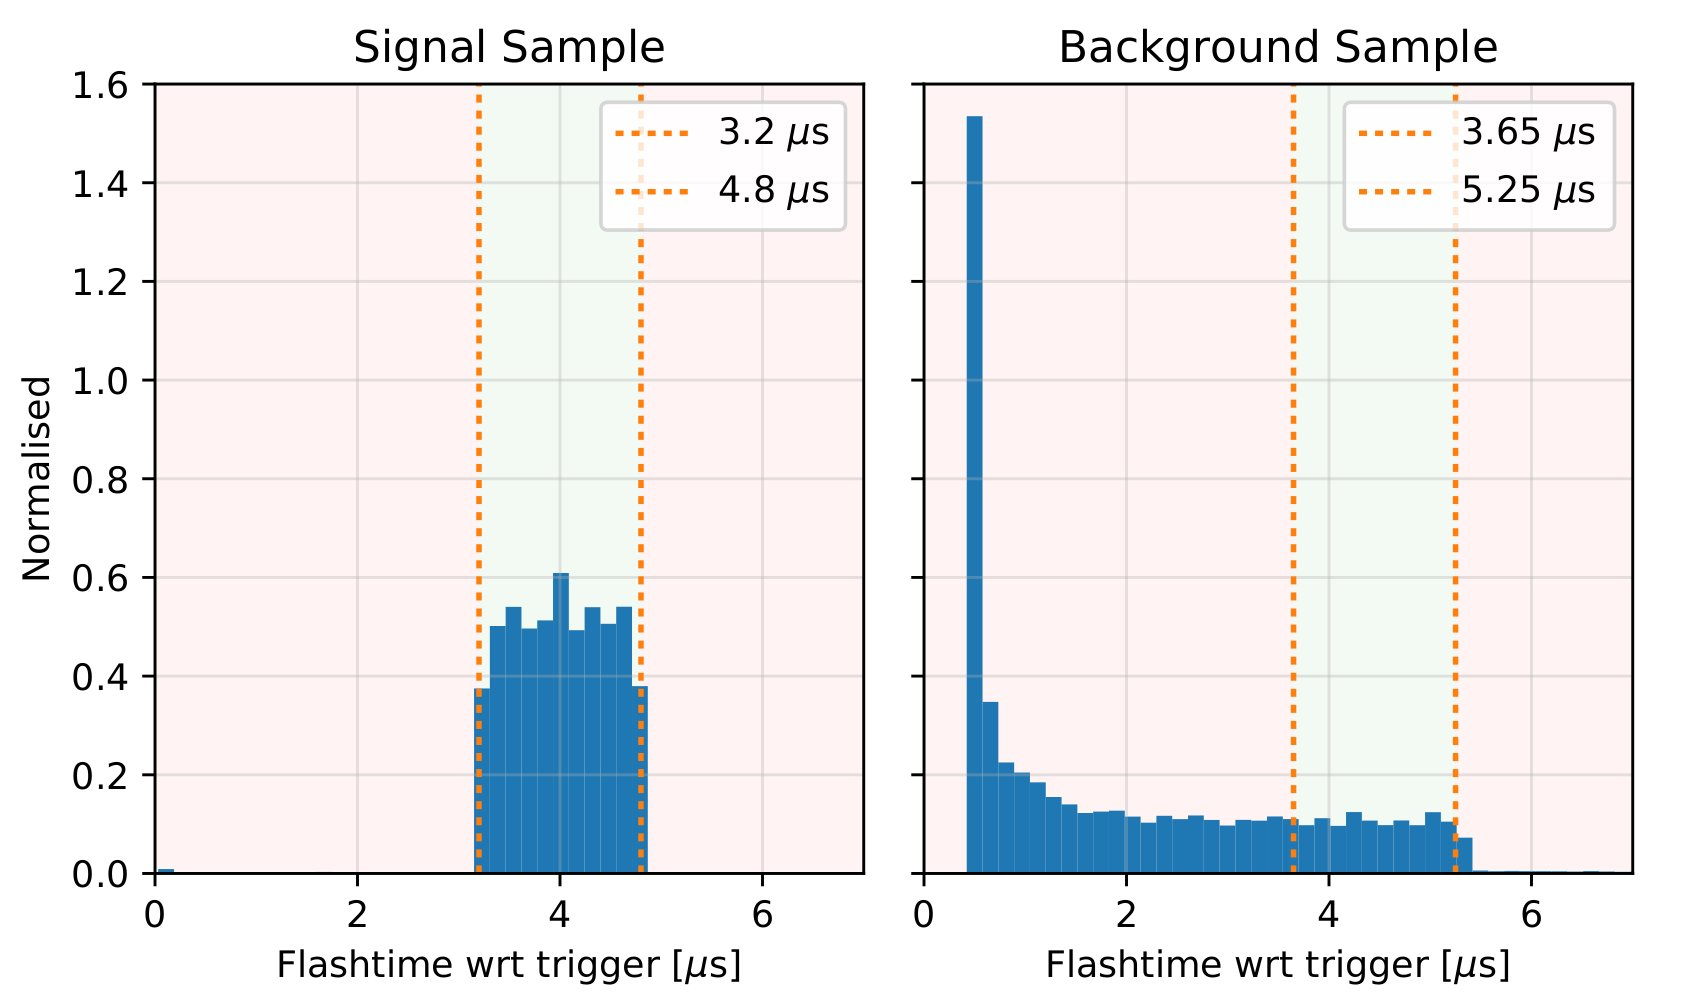
\includegraphics[width=0.75\textwidth]{beam}
\caption{Requirement a reconstructed flash object within the beam spill time window.} 
\label{fig:beam}
\end{figure}

The first requirement is that there is a reconstructed flash within the beam spill window of \SI{1.6}{\micro\s}. This cut is shown in Figure~\ref{fig:beam}. 99.6\% in the signal sample passes, 18.5\% in the background sample passes.

\begin{figure}[htbp]
\centering
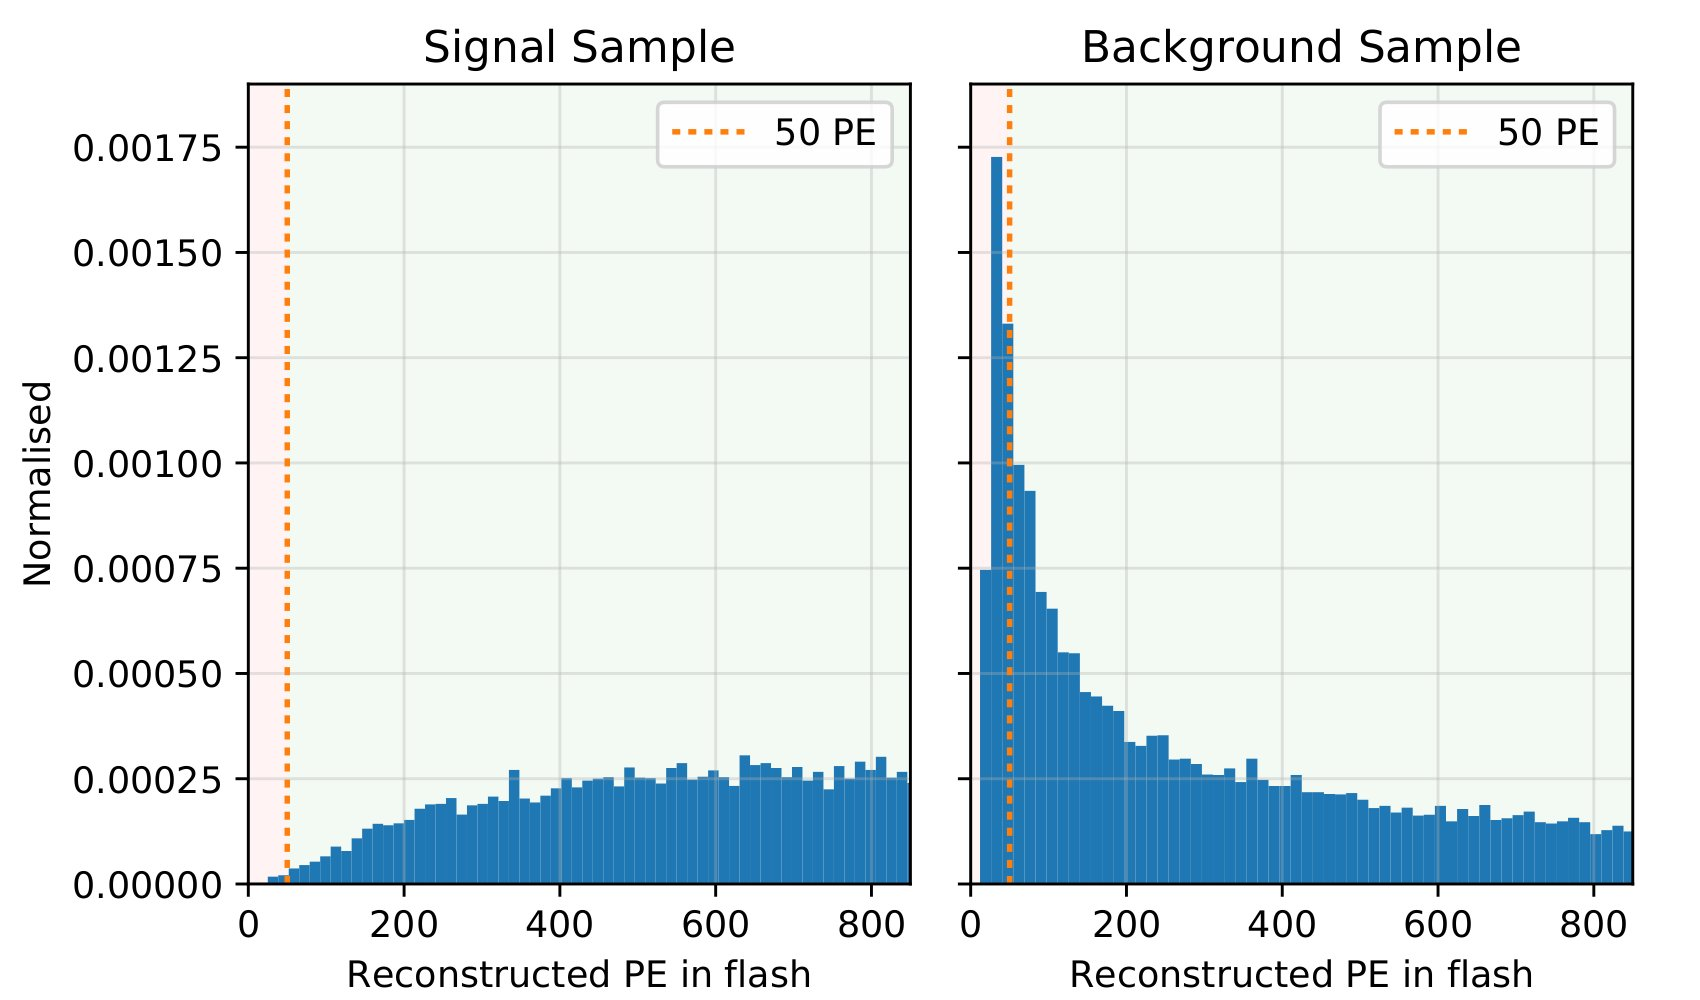
\includegraphics[width=0.75\textwidth]{PE}
\caption{Intensity of the reconstructed flash in photo-electrons. A cut is placed at 50 PE.} 
\label{fig:PE}
\end{figure}

After that, the reconstructed flash is required to consist of at least 50 photo-electrons (PE). This is a very conservative cut and keeps 99.95\% of the signal while 95.2\% of the background passes too. The PE distributions are given in Figure~\ref{fig:PE}.


\subsection{Optical Flash Matching}

At this point it is guaranteed that the event has a properly reconstructed flash. A flash object has a time and a PE count for each of the 32 PMT's. From that, a position $Z\pm \sigma_Z$ and $Y\pm \sigma_Y$ are calculated. These can be compared with the center of deposited charge of the Pandora candidate. This comparison has the implicit assumption that the light will be emitted in the same relative fraction as the charge is deposited by the final state particles. This is not completely correct since the amount of scintillation light produced per deposited \SI{1}{\MeV} is particle dependent. Nevertheless, compared to the coarse resolution of the PMT grid, this approximation is justified. 

\begin{figure}[htbp]
\centering
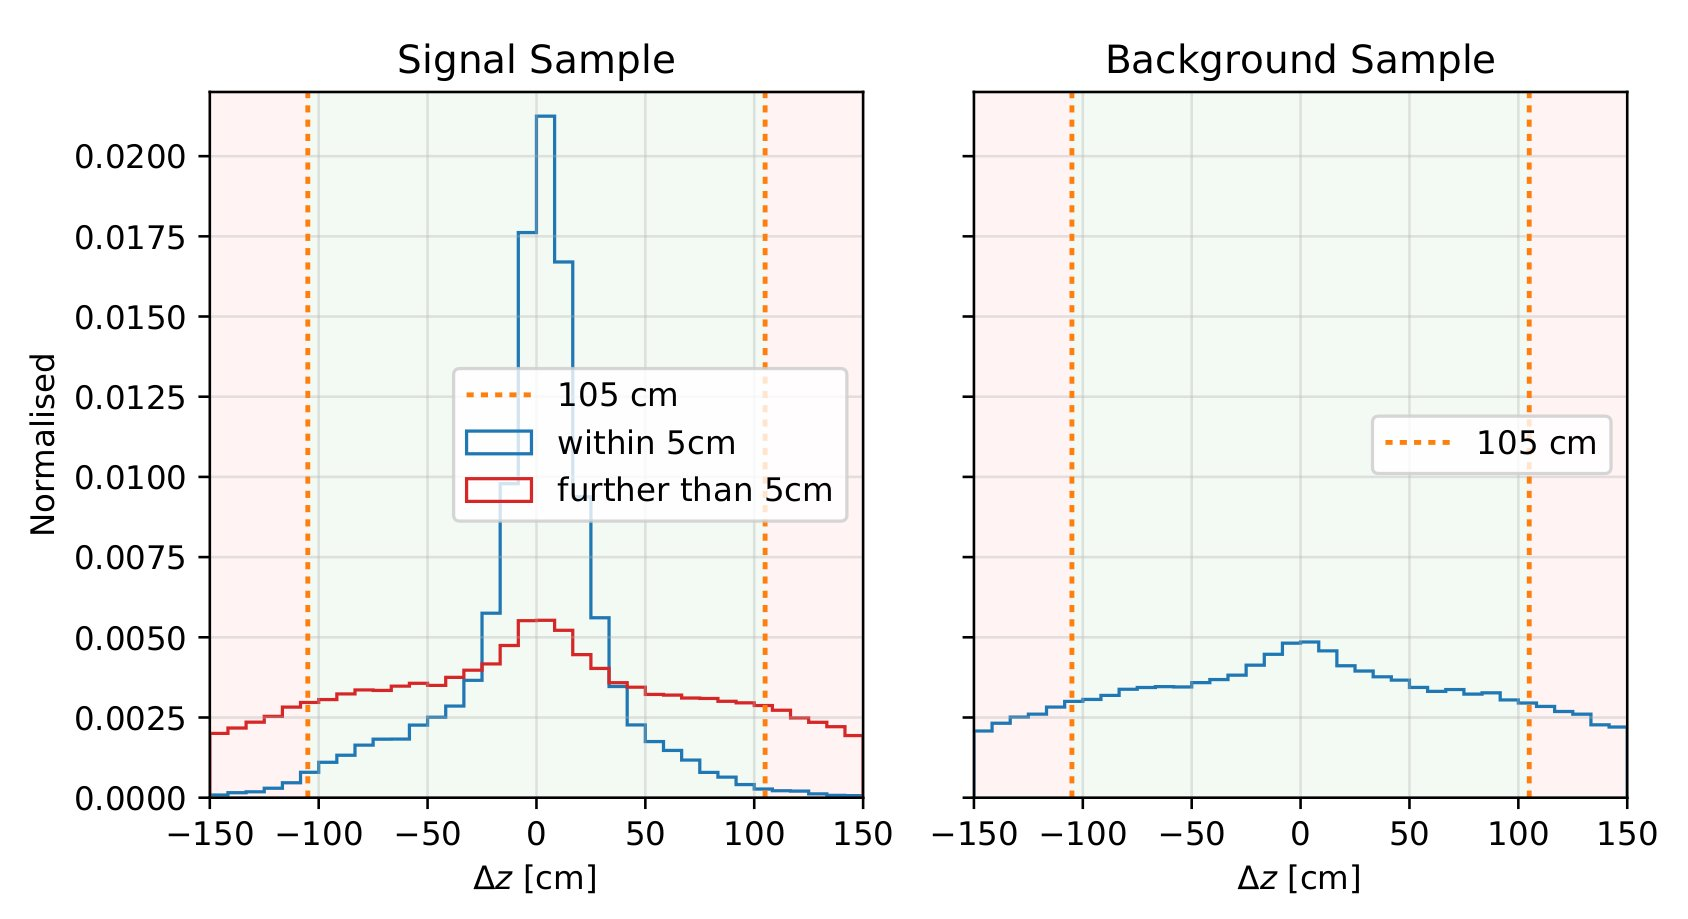
\includegraphics[width=0.8\textwidth]{zcut}
\caption{The distance between the flash and centre of deposited charge of the Pandora neutrino candidate. It is required that this is less than \SI{105}{\cm}.} 
\label{fig:zcut}
\end{figure}

In Figure~\ref{fig:zcut}, The effect of this cut is demonstrated. The signal sample is split up in two categories using truth information. Pandora neutrino candidates with their reconstructed vertex within \SI{5}{\cm} from the true vertex, and Pandora neutrino candidates with their reconstructed vertex further away. Those candidates with a mis-reconstructed vertex are often related to cosmic interaction, either mixed with neutrino activity or pure background. We therefore expect this group in the signal sample to follow the distribution of the background sample, which is confirmed in the figure. A cut is placed on a difference of \SI{105}{\cm} difference between the reconstructed flash position and the position of the deposited charge. This cut keeps at least one neutrino candidate in 98.1\% of the signal while it removes all neutrino candidates in 20\% of the background event. 
Similar cuts are obtained taking into account the width of the flash and the $y$-position. 

\begin{figure}[!htbp]
\centering
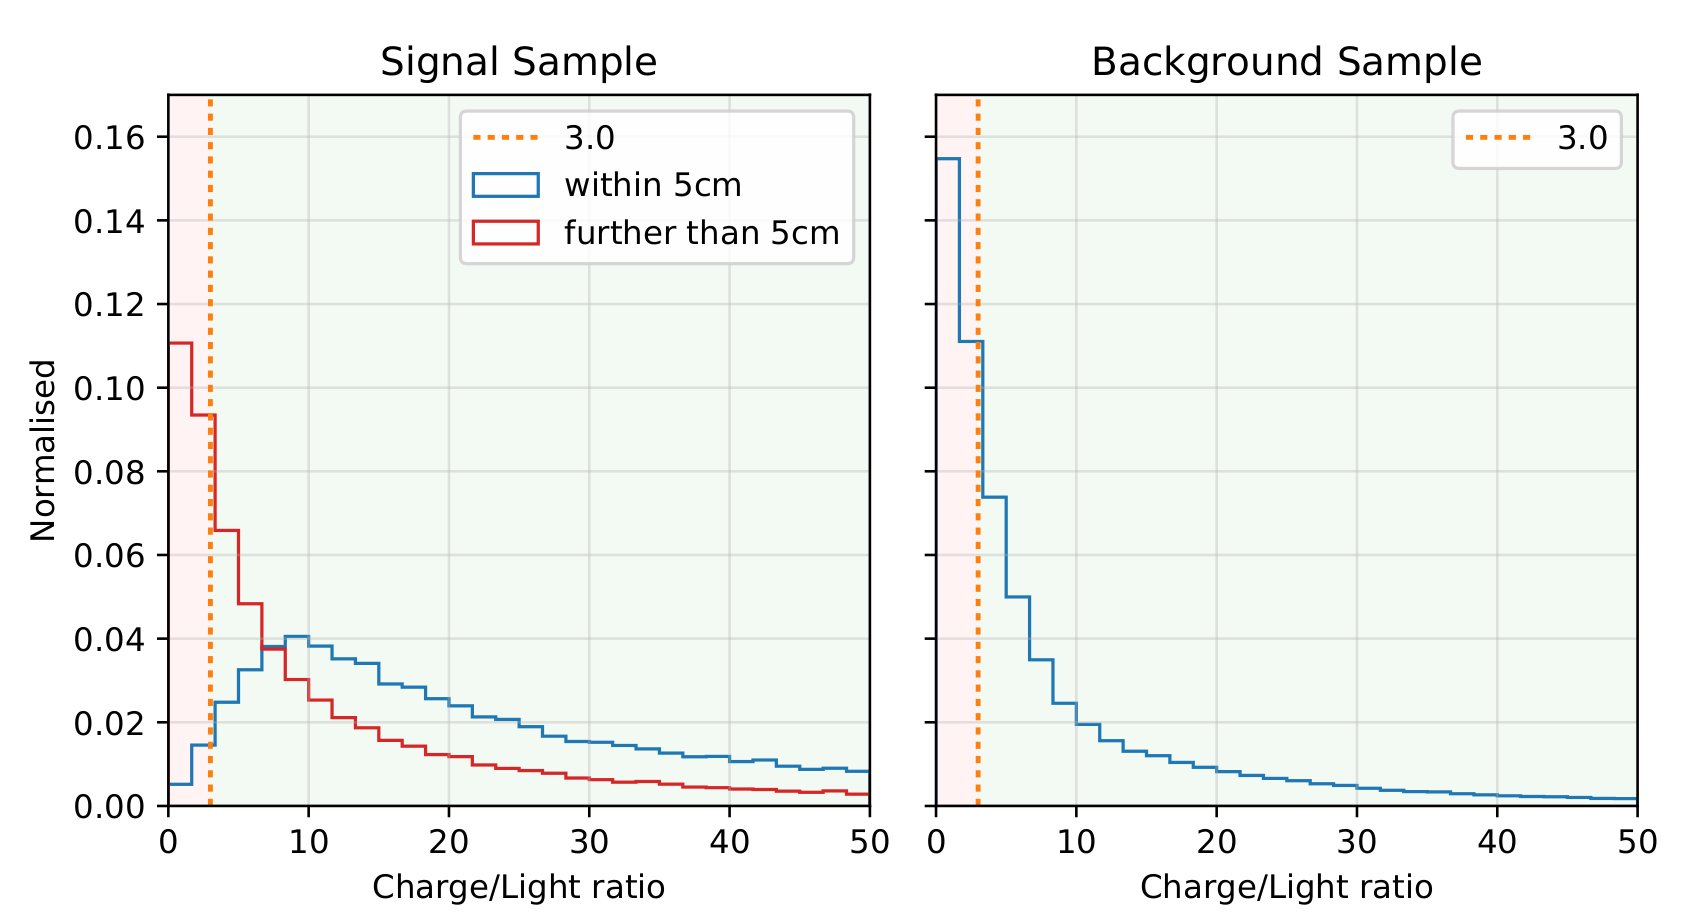
\includegraphics[width=0.8\textwidth]{charge}
\caption{For neutrino interactions, the a higher amount of deposited charge will come together with a more intense reconstructed flash. A cut on the ratio of higher than 3.0 is imposed on the neutrino candidates.} 
\label{fig:charge}
\end{figure}

The last rectangular cut exploits the fact that a lot of the neutrino candidates reconstructed by Pandora originate from remainders of cosmic activity that was not completely removed in the cosmic removal stage of the reconstruction. Those neutrino candidates often consist of a small amount of fragmented charge, incompatible with the brightness of the flash. In Figure~\ref{fig:charge}, the ratio of deposited charge associated to a neutrino candidate and the  amount of photo-electrons in the reconstructed flash is shown. The signal sample is again split up in two categories as before. Placing a very conservative cut at 3.0 reduces the signal events with a properly reconstructed flash with 1.7\% while removing all neutrino candidates in 15.4\% of the events. 

\begin{figure}[!htbp]
\centering
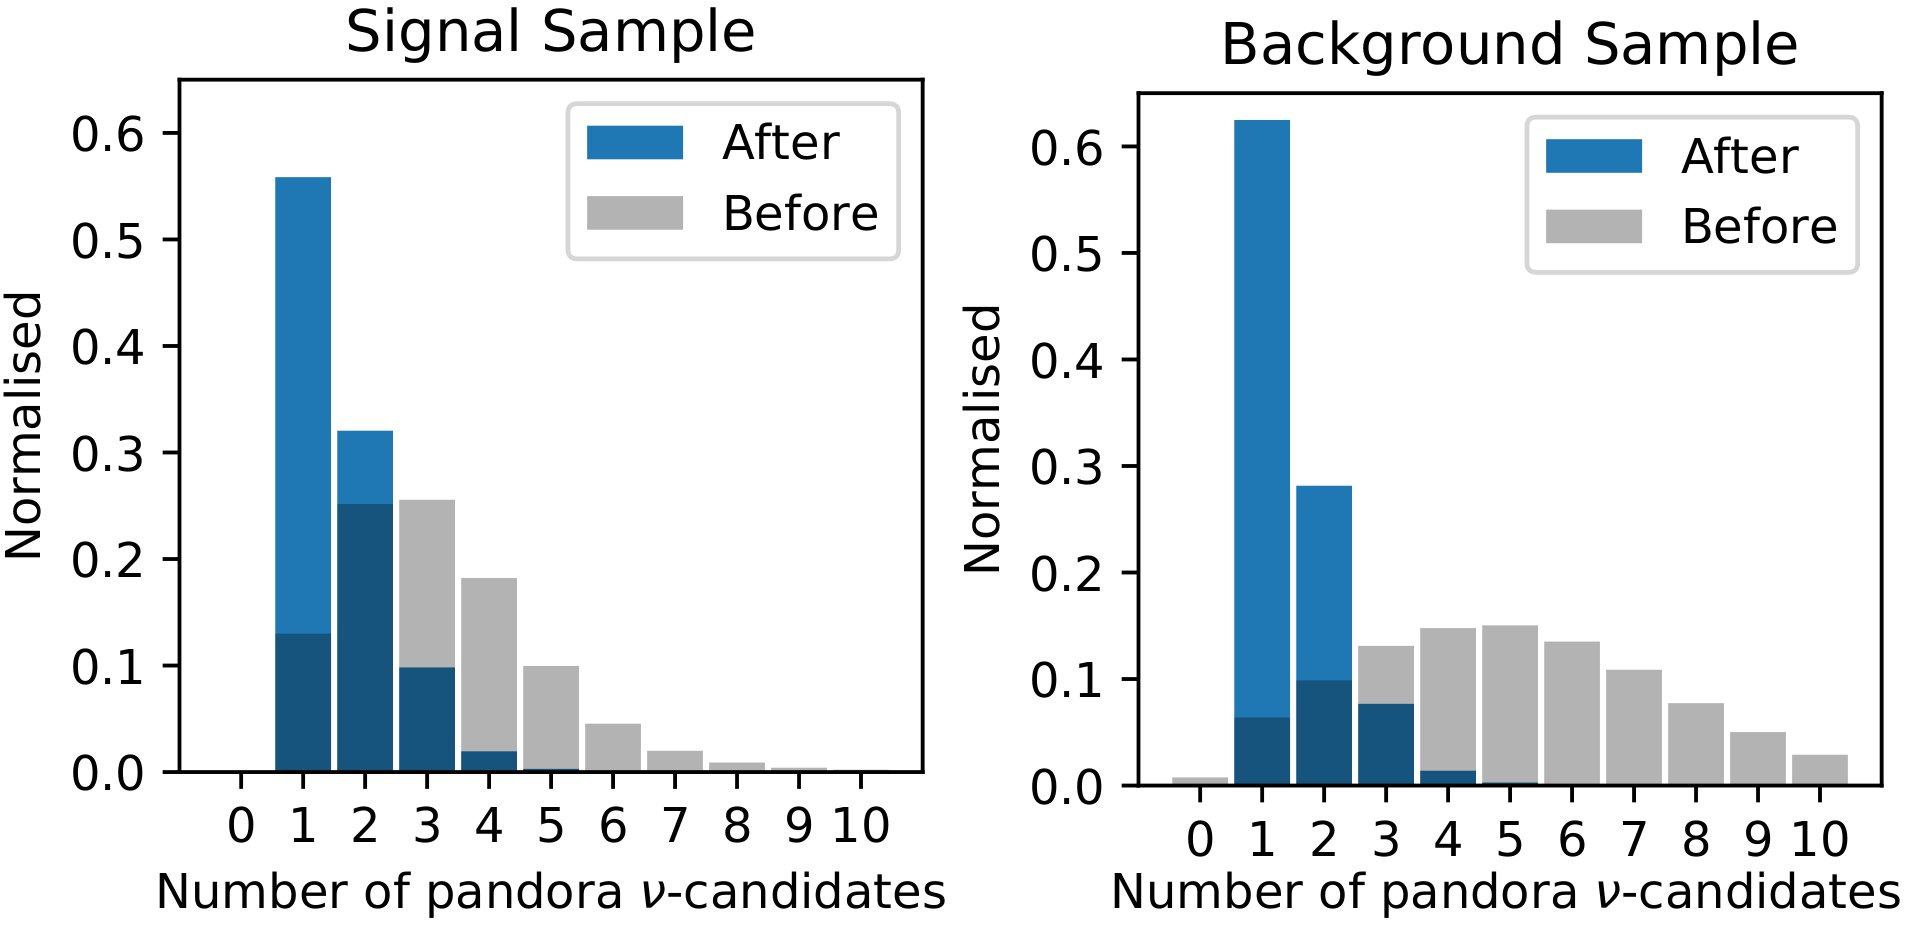
\includegraphics[width=0.8\textwidth]{boxed}
\caption{Effect of the rectangular optical cuts on the amount of Pandora neutrino candidates .} 
\label{fig:boxed}
\end{figure}

After applying the two sets of described rectangular cuts. It is informative to not only discuss the passing rates, but also the number of neutrino candidates remaining in the passed events. This is shown in Figure~\ref{fig:boxed}. In Grey, the number of neutrino candidates before any cuts is shown. In blue, the number of candidates that passed the rectangular cuts is shown. In about half of the remaining cases, there are multiple neutrino candidates remaining, this will be reduced to exactly one per passing event using flash-matching. 

\begin{figure}[!htbp]
\centering
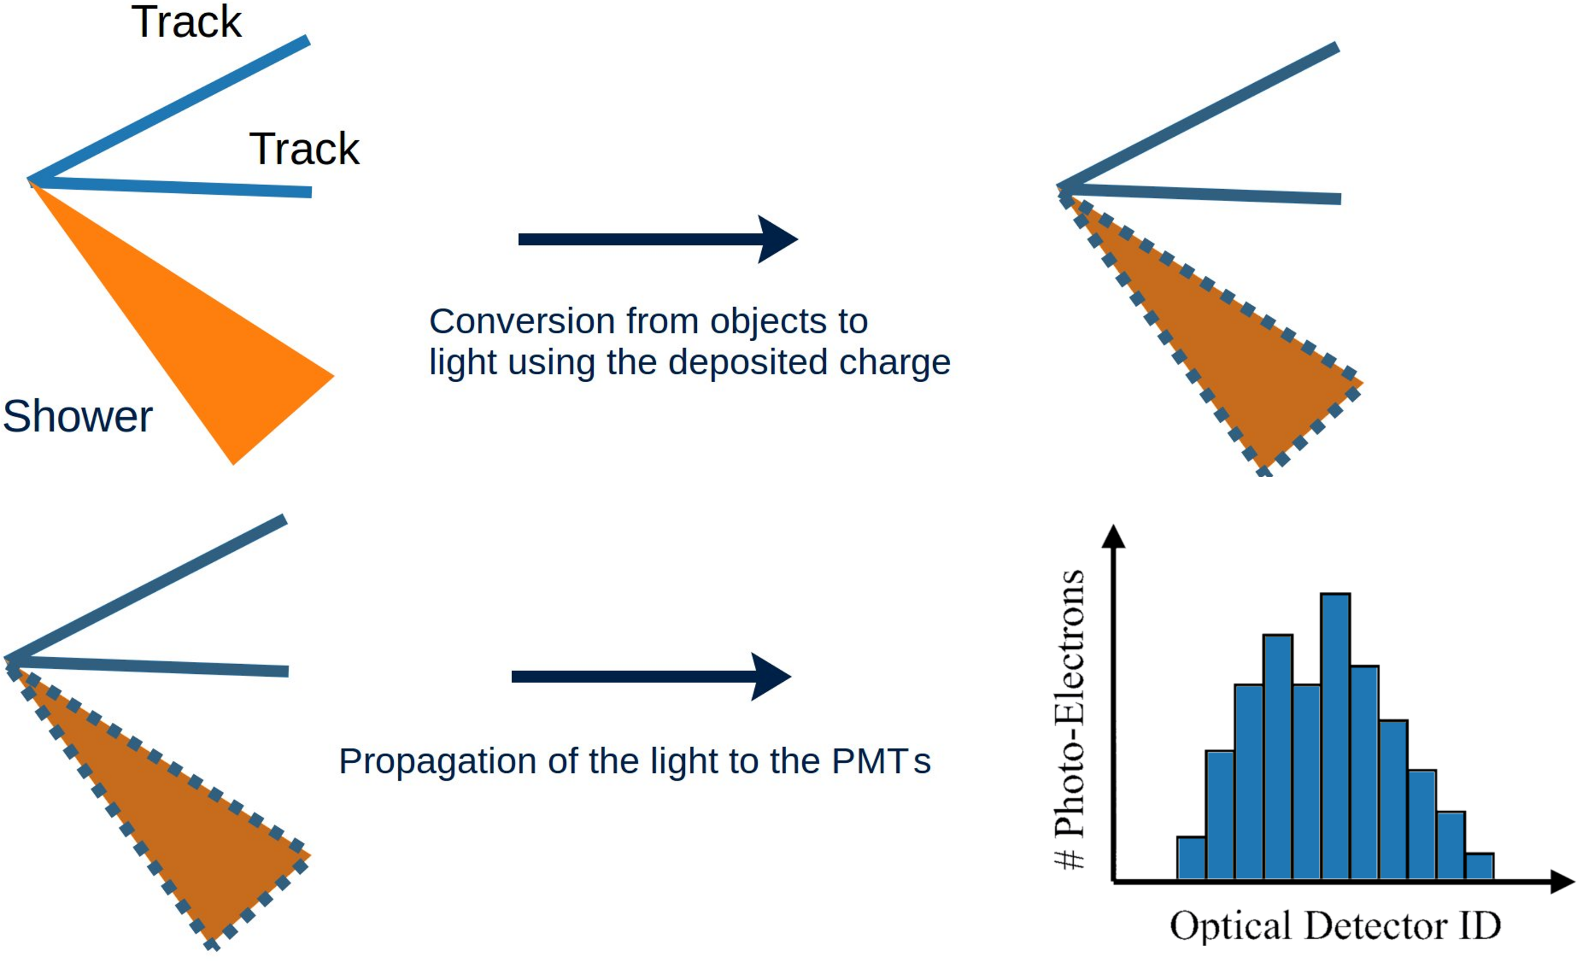
\includegraphics[width=0.7\textwidth]{flashdrawing} 
\caption{Schematic of the construction of a flash hypothesis for a neutrino candidate.} 
\label{fig:flashdrawing}
\end{figure}

The principle of flash-matching is described in Figure~\ref{fig:flashdrawing}:
\begin{itemize}
\item A flash hypothesis can be constructed for each candidate vertex using only data recorded by the time projection chamber.
\item For every neutrino candidate, a spatial distribution of deposited charge can be constructed.
\item The spatial distribution of the deposited charge is translated into an estimation of the emitted scintillation light. These scintillation photons are then propagated towards the PMTs to construct a flash hypothesis using only time projection chamber information.
\item The flash-matching algorithm compares the reconstructed flash object as seen by the PMT's with the hypothetical flash for all possible neutrino candidates and picks the best matching candidate. For this, a binned likelihood of the PMT spectrum is optimised.
\end{itemize}
An example of this procedure for a Monte Carlo generated $\nu_e$ event with 4 neutrino candidates is given in Figure~\ref{fig:flashmatch}.
\begin{figure}[!htbp]
\centering
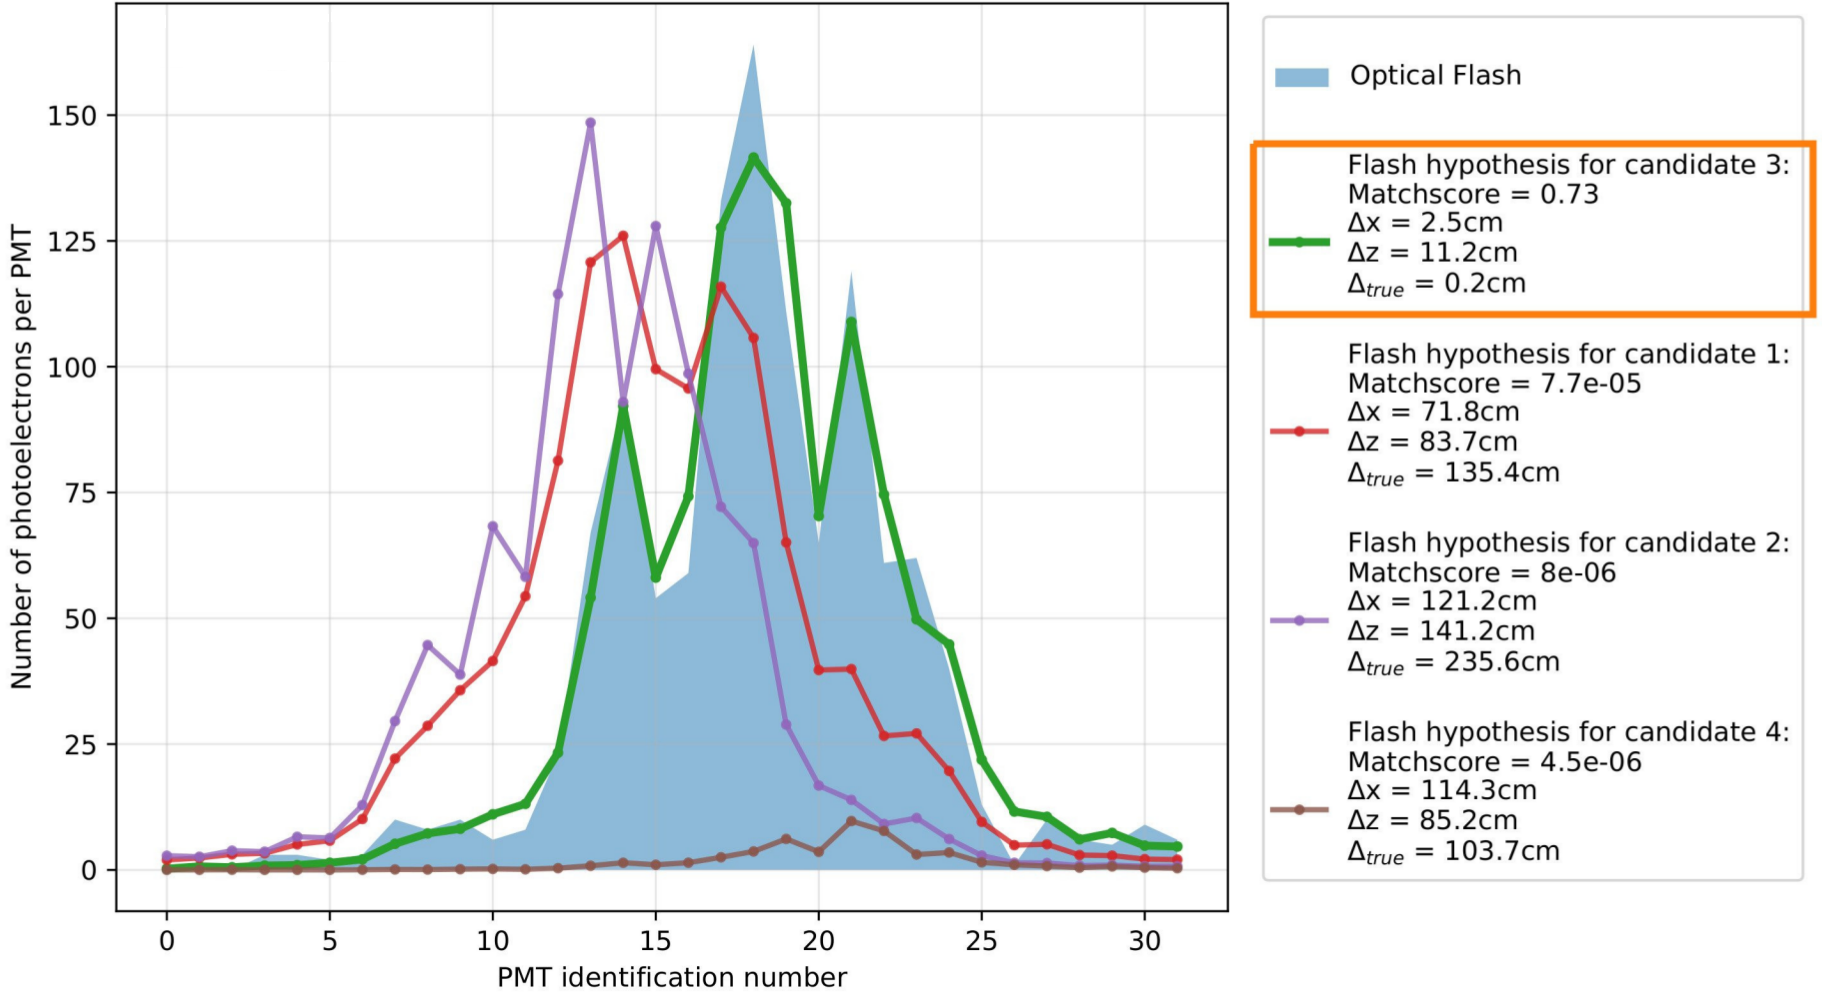
\includegraphics[width=0.85\textwidth]{flashmatch} 
\caption{An example of flash-matching. Event with 4 neutrino candidates, for all of the candidates the flash hypothesis is constructed and matched to the reconstructed flash (shaded blue). For all candidates a minimum binned likelihood is calculated, varying the $x$ position of the interaction. The match score is the inverse of the likelihood. For all neutrino candidates, the reconstructed vertex is compared with the true distance and given by $\Delta_{true}$ } 
\label{fig:flashmatch}
\end{figure}

\subsection{Electron Neutrino Topological Pre-Selection} \label{sec:topological_pre_selection}
A perfect reconstruction of a $\nu_{e}$ CC0$\pi$-Np event in a LArTPC will produce as many reconstructed tracks as the number of protons in the final state and a single reconstructed shower (the electron), sharing a common vertex. However, the presence of missing or unresponsive wires can cause the splitting of an ionization track or an electromagnetic showers into two distinct reconstructed object. Also, the type of object (track or shower) is assigned by a Support Vector Machine (SVM) implemented in the Pandora framework and its performances depend on the quality of the event (e.g. the number of hits). A track-like object (e.g. a proton or a muon), then, can be mis-reconstructed as a shower-like object, especially when the number of reconstructed hits is low \cite{pandora2}. In order to maximize our efficiency, then, we will require (1) \emph{at least} one track and \emph{at least} one shower sharing a common vertex, or (2) \emph{at least} two showers sharing a common vertex. Figure \ref{fig:dia} shows the two diagrams of the accepted topologies for a $\nu_{e}$ CC0$\pi$-Np candidate event.

\begin{figure}[htbp]
\centering
  \begin{subfigure}{0.4\textwidth}
    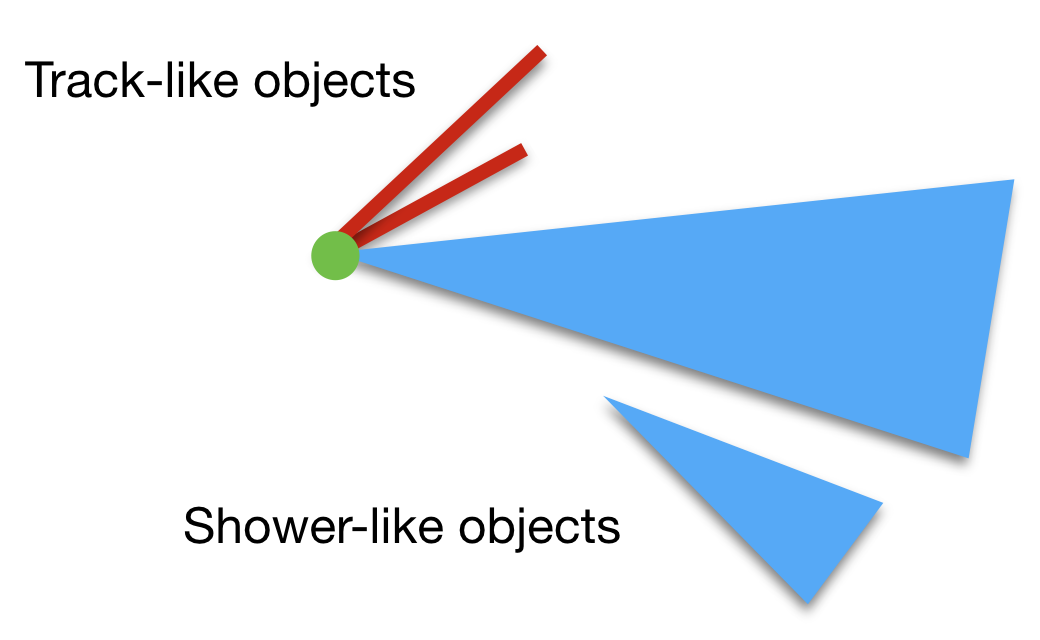
\includegraphics[width=\linewidth]{figures/trsh.png}
    \caption{1+ tracks and 1+ showers} 
  \end{subfigure}
    \begin{subfigure}{0.4\textwidth}
    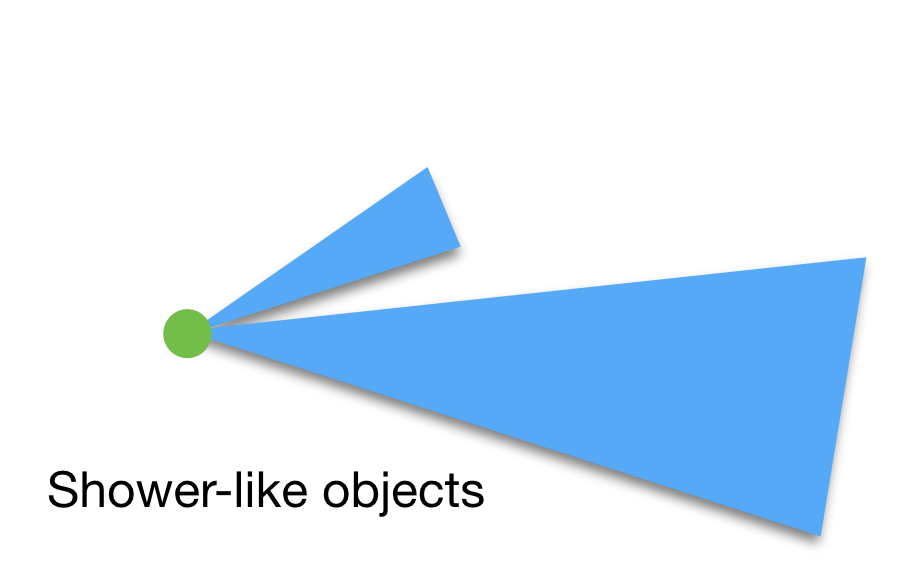
\includegraphics[width=\linewidth]{figures/sh.png}
    \caption{2+ showers} 
  \end{subfigure}
  \caption{The $\nu_{e}$ topological pre-selection requires a neutrino candidate with one or more tracks and one or more shower sharing (left) or two or more showers (right) sharing  a common vertex.}\label{fig:dia}
\end{figure}

Figure \ref{fig:2showers} shows a Monte Carlo event display with an electromagnetic shower correctly reconstructed as a shower-like object and a proton track mis-reconstructed as a shower-like object. Requiring at least two showers allows to recover this kind of event.

\begin{figure}[htbp]
	\begin{center}
    	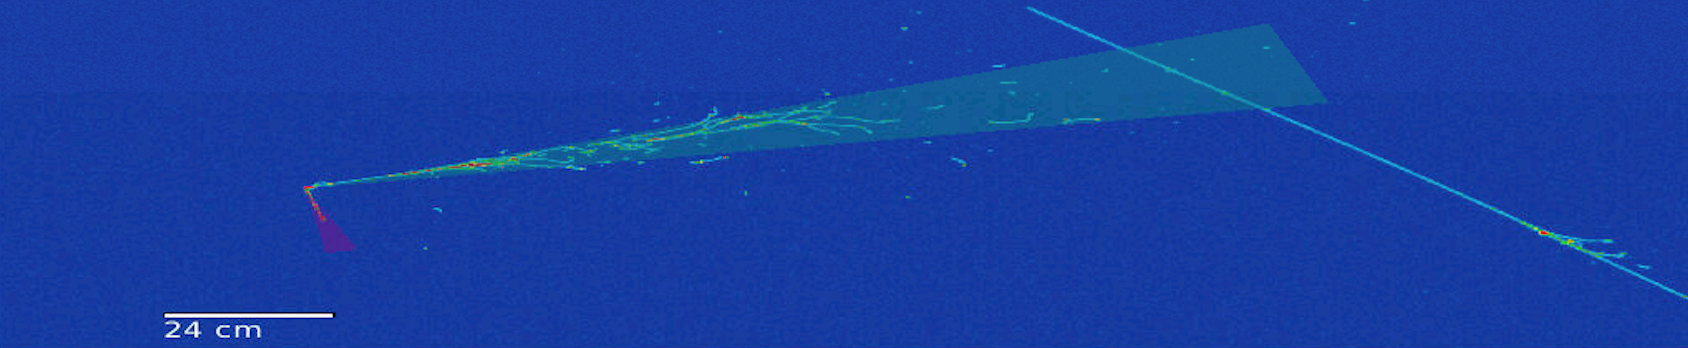
\includegraphics[width=0.8\linewidth]{figures/2showers.png}
    	\caption{Monte Carlo event display of the collection plane with one electron and one proton in the final state. The proton track has been mis-reconstructed as a shower-like object.} \label{fig:2showers}
	\end{center}
\end{figure}

In these cases, in order to choose the proton track candidate among the two or more shower-like objects, we run a bi-dimensional Principal Component Analysis in the collection plane (one dimension is given by the drift time and the other by the wire coordinate). The object with the largest first eigenvalue is chosen as the proton track candidate and it is then considered as a track-like object.

\subsubsection{Selection efficiency and purity}\label{sec:eff}
A first estimate of the number of events that can be selected by our algorithm is obtained by measuring the selection efficiency and purity using a dedicated $\nu_{e}$ CC$0\pi$-Np Monte Carlo sample. Neutrino events have been generated using the GENIE Neutrino Monte Carlo generator \cite{genie} and cosmic rays have been generated using the CORSIKA Monte Carlo generator \cite{corsika}. 

In this sample, every event has one $\nu_{e}$ interaction with one electron, at least one proton and no other visible particles in the final state (it can have neutrons). 

In order to avoid border effects, such as electric field non-uniformities, the true neutrino interaction vertex must lie within a fiducial volume. Our fiducial volume cut is $\pm10$~cm on the $x$ axis, $\pm20$~cm on the $y$ axis, and $^{+10}_{-50}$~cm on the $z$ axis. 
Since electromagnetic showers develop mainly in the forward direction with respect to the beam, the asymmetric cut on the $z$ axis (which corresponds to the beam direction) helps reject non-fully contained events.

A study on the reconstruction efficiency of proton tracks and electron showers in $\nu_{e}$ CC$0\pi$-Np events shows that the efficiency is zero for proton with a kinetic energy below 40~MeV and for electrons with a kinetic energy below 20~MeV. The efficiency has been calculated by counting the number of reconstructed electrons or protons (regardless of their shower-like or track-like identification), divided by the number of generated protons and electrons. In the case of events with more than one proton, each proton has been counted individually.

As such, in our sample each event must have at least one proton above 40~MeV and one electron above 20~MeV. Figure \ref{fig:kin_eff} shows the reconstruction efficiencies for simulated protons and electrons as a function of their generated kinetic energy, between 0 and 200 MeV.

\begin{figure}[htbp]
  \begin{subfigure}{0.48\textwidth}
    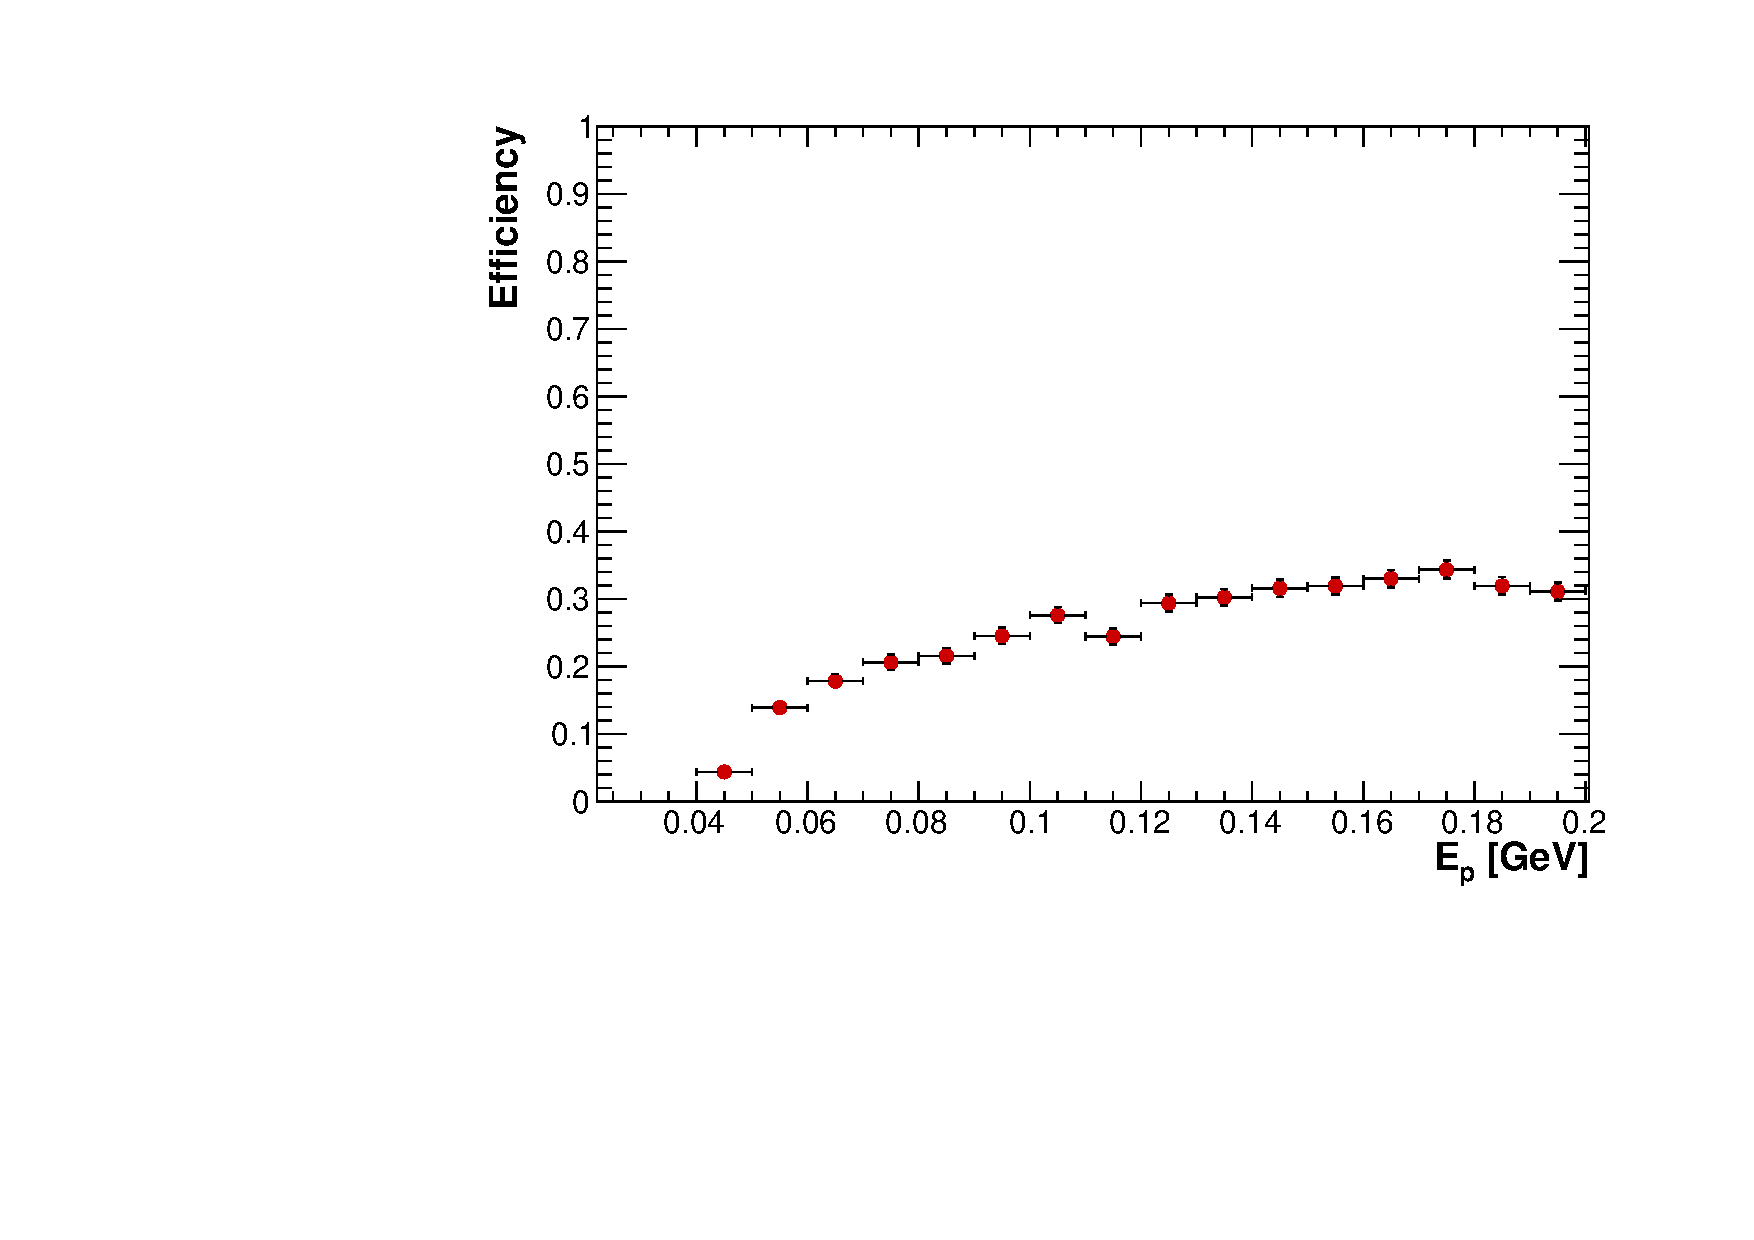
\includegraphics[width=\linewidth]{figures/proton_eff.pdf}
    \caption{Proton reconstruction efficiency} 
  \end{subfigure}
    \begin{subfigure}{0.48\textwidth}
    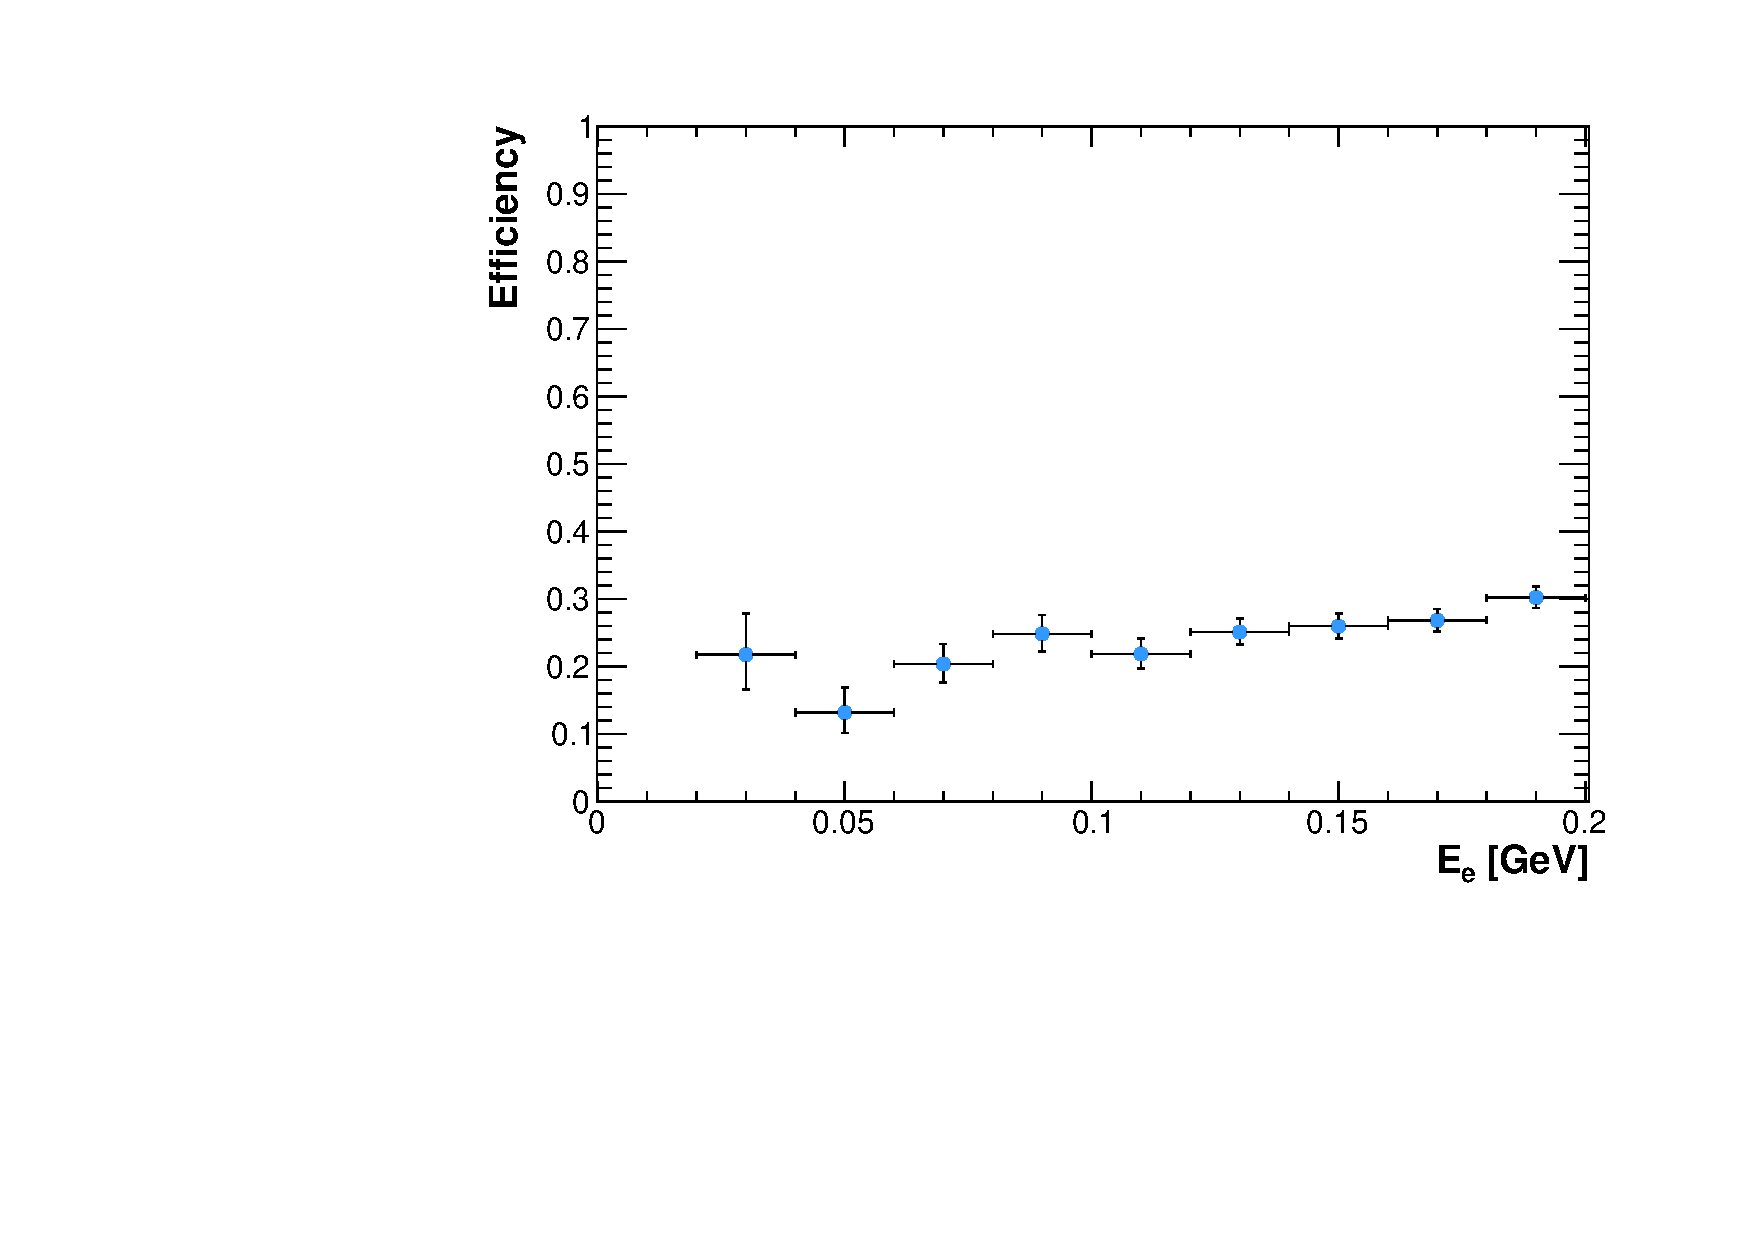
\includegraphics[width=\linewidth]{figures/electron_eff.pdf}
    \caption{Electron reconstruction efficiency} 
  \end{subfigure}
  \caption{Proton (left, in red) and electron (right, in blue) reconstruction efficiency for simulated $\nu_{e}$ CC$0\pi$-Np events. In our sample of generated $\nu_{e}$ CC$0\pi$-Np events we require at least one proton above 40~MeV and at least an above 20~MeV.}
  \label{fig:kin_eff}
\end{figure}


The selection efficiency $\epsilon$ is defined as:
\begin{equation}
\epsilon = \frac{\mathrm{N.~of~selected~CC0}\pi\mathrm{{\text -}Np~events}}{\mathrm{N.~of~generated~CC0}\pi\mathrm{{\text -}Np~events}},
\end{equation}
where each selected event must pass the optical selection and satisfy the topology requirement. A minimum quality of the selected event is also ensured requiring (1) at least 5 hits in the collection plane associated to a shower-like object, (2) at least 5 hits in the collection plane associated to a track-like object, and (3) at least one hit in every plane.
The start and end point of each track-like object and the start point of each shower-like object must also lie within the fiducial volume to ensure that the event is fully contained.

The purity of the sample is defined as:
\begin{equation}
P = \frac{\mathrm{N.~of~selected~CC0}\pi\mathrm{{\text -}Np~events}}{\mathrm{N.~of~selected~events}},
\end{equation}
and it has been measured running the selection algorithm on a complete sample of neutrino events (not only $\nu_{e}$ interactions), weighted accordingly to the Booster Neutrino Beam (BNB) flux. In this sample every event will have at least one neutrino interacting in the cryostat volume and triggering the detector, plus all the cosmic rays hitting the detector in the same readout window. In the data, however, this is not always true, since the detector can be triggered also by a cosmic ray producing a flash in the optical system during the beam window, without necessarily having a neutrino interaction. In order to estimate this background component, defined as \emph{in-time cosmic rays}, we have used the data EXT sample, which was collected using the standard detector trigger, but with the neutrino beam off.

Figure \ref{fig:effpurity} shows the efficiency as a function of the true neutrino energy and the purity as a function of the reconstructed energy. The energy reconstruction procedure is described in section \ref{sec:energyreco}.
As expected, the efficiency (purity) is proportional to the neutrino energy (reconstructed energy), since high-energy events correspond in general to a larger number of hits in the TPC and the Pandora framework reconstruction performances are proportional to the number of reconstructed hits 
\cite{pandora2}. 

\todo{Add efficiency plots over a larger energy region for protons and electrons.}

\begin{figure}
  \begin{subfigure}{0.48\textwidth}
    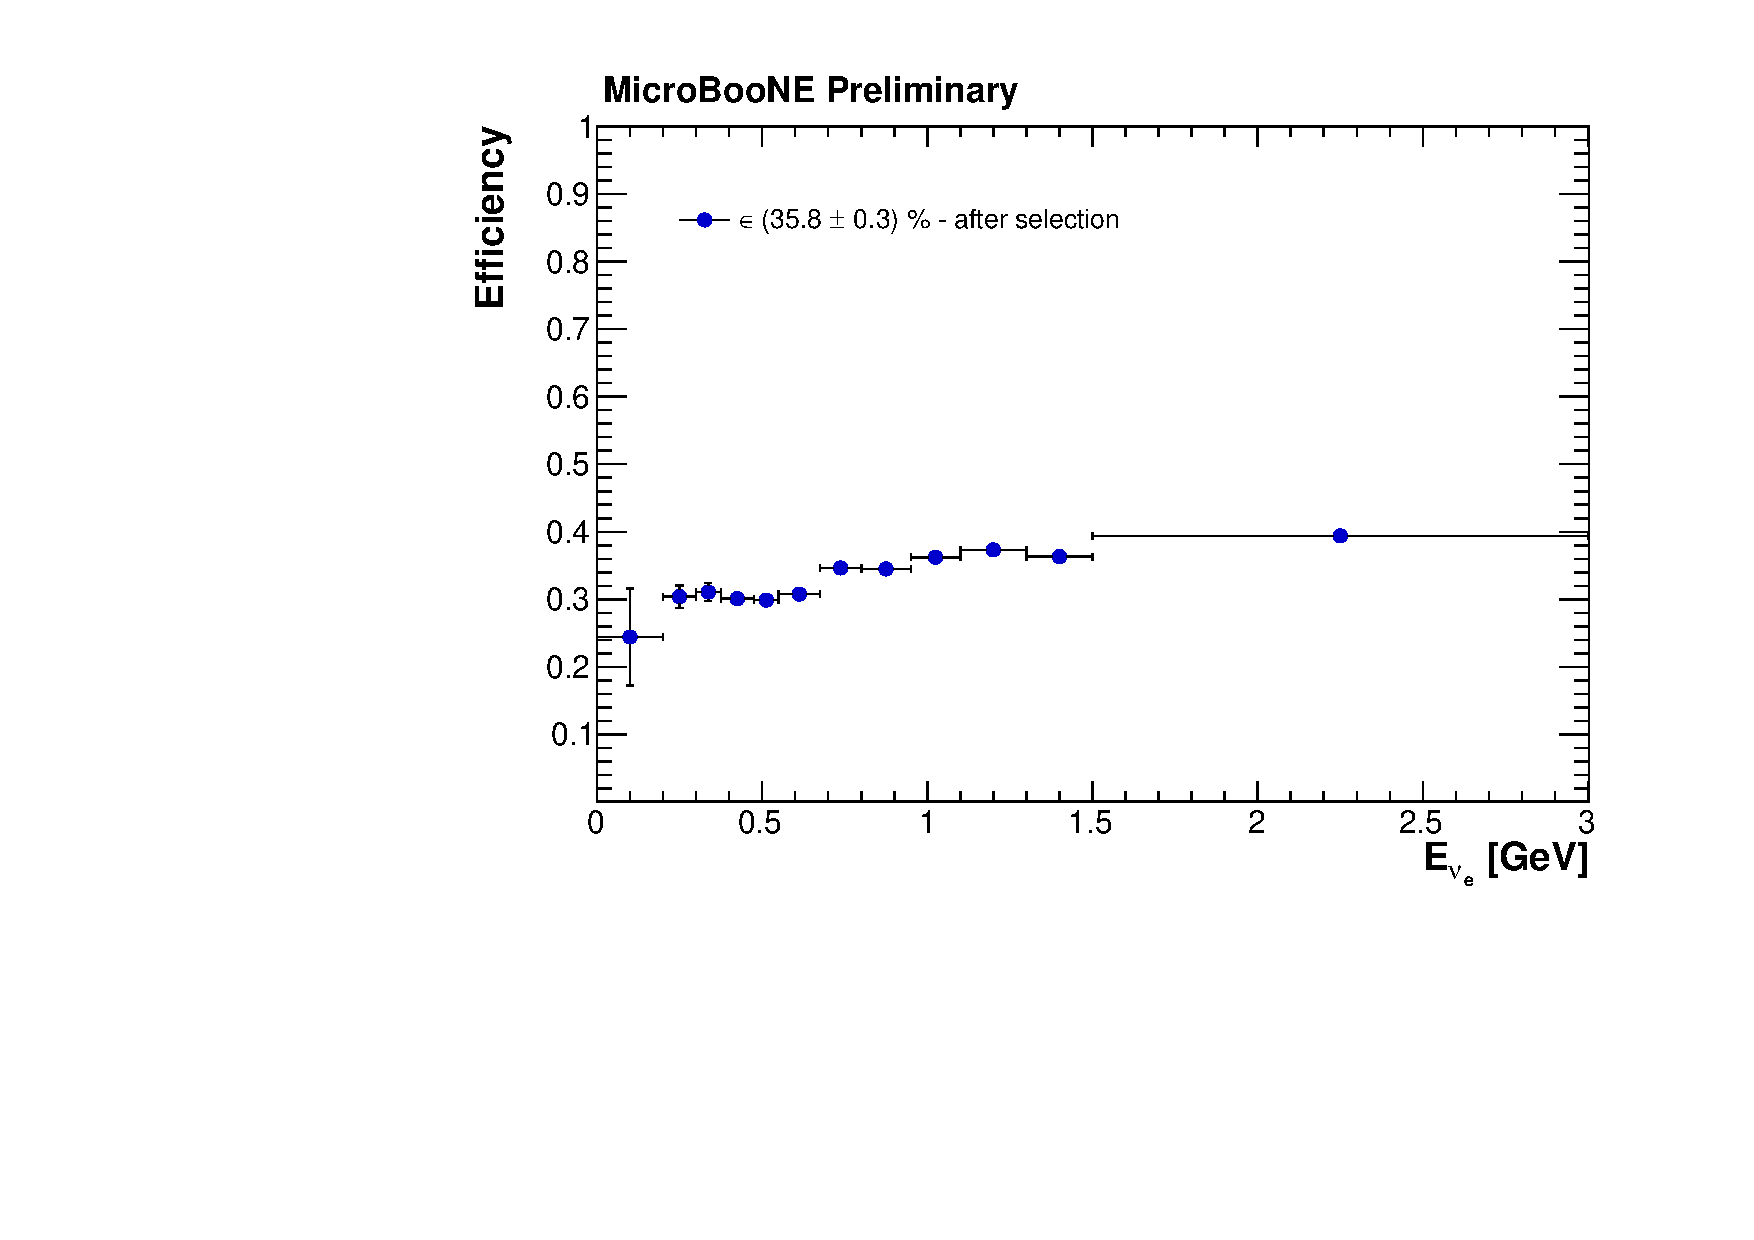
\includegraphics[width=\linewidth]{figures/eff.pdf}
    \caption{Efficiency} 
  \end{subfigure}
    \begin{subfigure}{0.48\textwidth}
    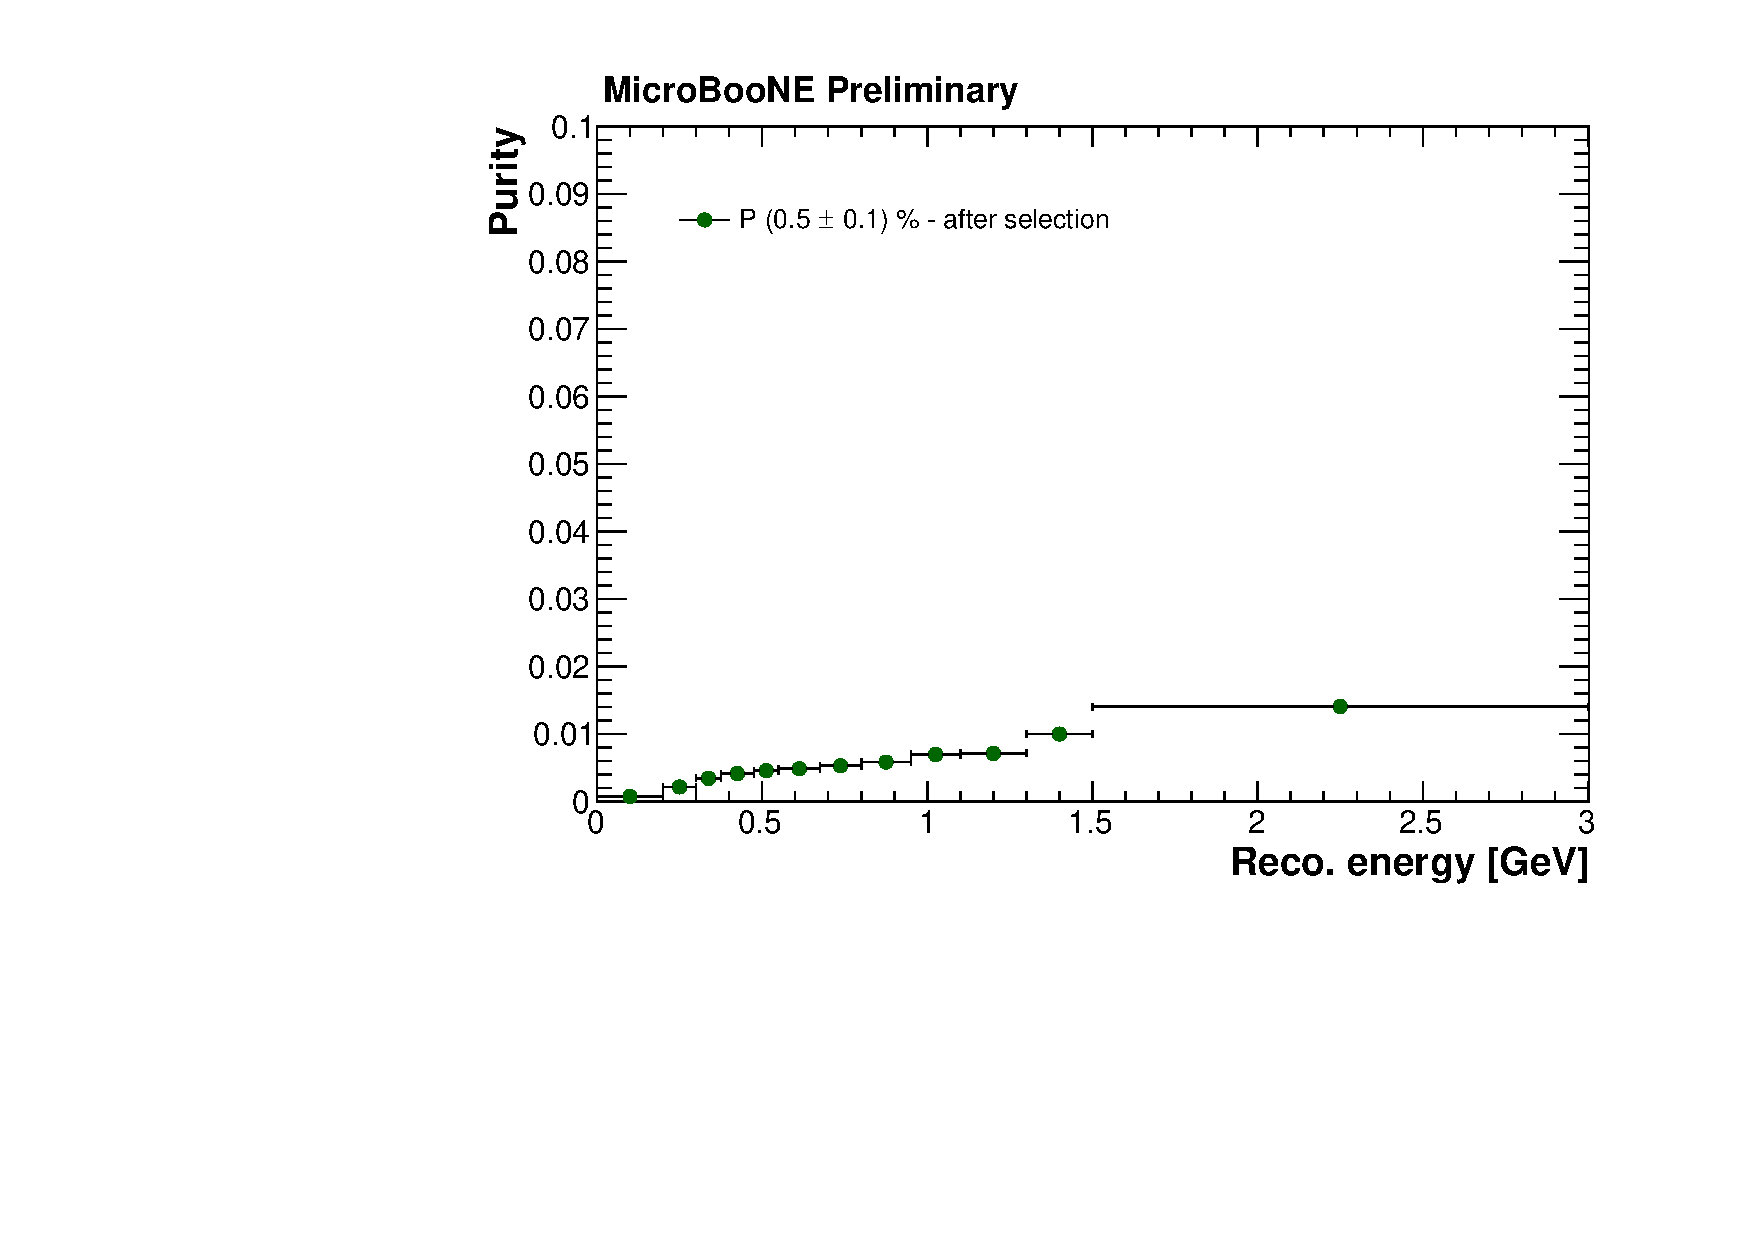
\includegraphics[width=\linewidth]{figures/purity.pdf}
    \caption{Purity} 
  \end{subfigure}
  \caption{Left: $\nu_{e}$ CC$0\pi$-Np reconstruction efficiency as a function of the true $\nu_{e}$ energy. Right: $\nu_{e}$ CC$0\pi$-Np purity as a function of the reconstructed energy.}
  \label{fig:effpurity}
\end{figure}

In order to understand the different background components, we divided our sample of selected events into further 8 categories:
\begin{description}
\item[Beam intrinsic $\nu_{e}$ CC$0\pi$-Np] charged-current $\nu_{e}$ neutrino interaction with no pions in the final state and at least one proton (N > 1).
\item[Beam intrinsic $\nu_{e}$ CC] charged-current $\nu_{e}$ neutrino interaction that is not in the $\nu_{e}$ CC$0\pi$-Np channel.
\item[Beam intrinsic $\nu_{\mu}$] charged-current $\nu_{\mu}$ neutrino interaction.
\item[Beam intrinsic NC] neutral current neutrino interaction (both $\nu_{\mu}$ and $\nu_{e}$).
\item[Outside fid. vol.] the true neutrino interaction happen outside the fiducial volume, but one or more final-state particles produce a reconstructed neutrino candidate inside in the fiducial volume.
\item[Cosmic] there is a neutrino interaction in the event, but the cosmic-ray interaction happening during the same drift time is selected instead.
\item[Cosmic in-time] there is no neutrino interaction in the event and a cosmic-ray interaction happening inside the beam gate time window is selected. It corresponds to the data EXT sample.
\item[Cosmic contaminated] the neutrino interaction candidate contains at least a track or a shower generated by a cosmic ray.
\end{description}


Table \ref{tab:result} shows a summary of the selection algorithm results, with the corresponding number of events for each category. The numbers correspond to an exposure of the MicroBooNE detector of \num{4.84e19} protons on target (POT), which is the amount of data available in the open sample.

\begin{table}[htbp]
   \centering
   \begin{tabular}{llrrrrr}
     \toprule
     Category & \phantom{a} & Generated & \phantom{a} & Selected & \phantom{a} & Efficiency \\
     \midrule

     $\nu_{e}$ CC0$\pi$-Np       & & 34.8     & & 14.3   & & 41.1\%\\
     $\nu_{e}$ CC                & & 35.7     & & 13.2   & & 37.0\%\\
     Beam intrinsic $\nu_{\mu}$  & & 11337.4  & & 918.3  & & 8.1\%\\
     Beam intrinsic NC           & & 3633.9   & & 342.2  & & 9.4\%\\
     Outside fid. vol.           & & 2609.5   & & 37.1   & & 1.4\%\\
     Cosmic in-time              & & 135377.2 & & 1151.6 & & 0.9\%\\
     Cosmic contaminated         & & -        & & 260.7  & & -\\
     Cosmic                      & & -        & & 233.3  & & -\\

     \bottomrule
   \end{tabular}
   \caption{Summary of the selection algorithm results, showing the contribution of each event category, for a MicroBooNE exposure of \num{4.84e19} POT.}\label{tab:result}
\end{table}


\subsection{CC \texorpdfstring{$\nu_{\mu}$}{numu} Event Rejection}\label{sec:numu}
The module \texttt{UBXSec} \cite{ubxsec} looks for charged-current $\nu_{\mu}$ candidates and it also helps reject cosmic-induced background events.  Figure \ref{fig:spectrum} shows the reconstructed energy spectrum obtained vetoing the events that \texttt{UBXSec} flagged as CC $\nu_{\mu}$ candidates or cosmic-induced background. The reconstructed energy has been measured with the procedure described in Section \ref{sec:energyreco}, after reclassifying the reconstructed Pandora objects as described in Section \ref{sec:reclass}. The ratio between the number of data events and the number of Monte Carlo events (POT normalized) is 1 and the low value of the $\chi^{2} / \mathrm{n.d.f.}$ (1.06) shows that the two distributions agree also in shape. This plot also shows that our selection procedure has similar performances in data and Monte Carlo and that there is no evident bias in the energy reconstruction. 

\begin{figure}[htbp]
\centering
  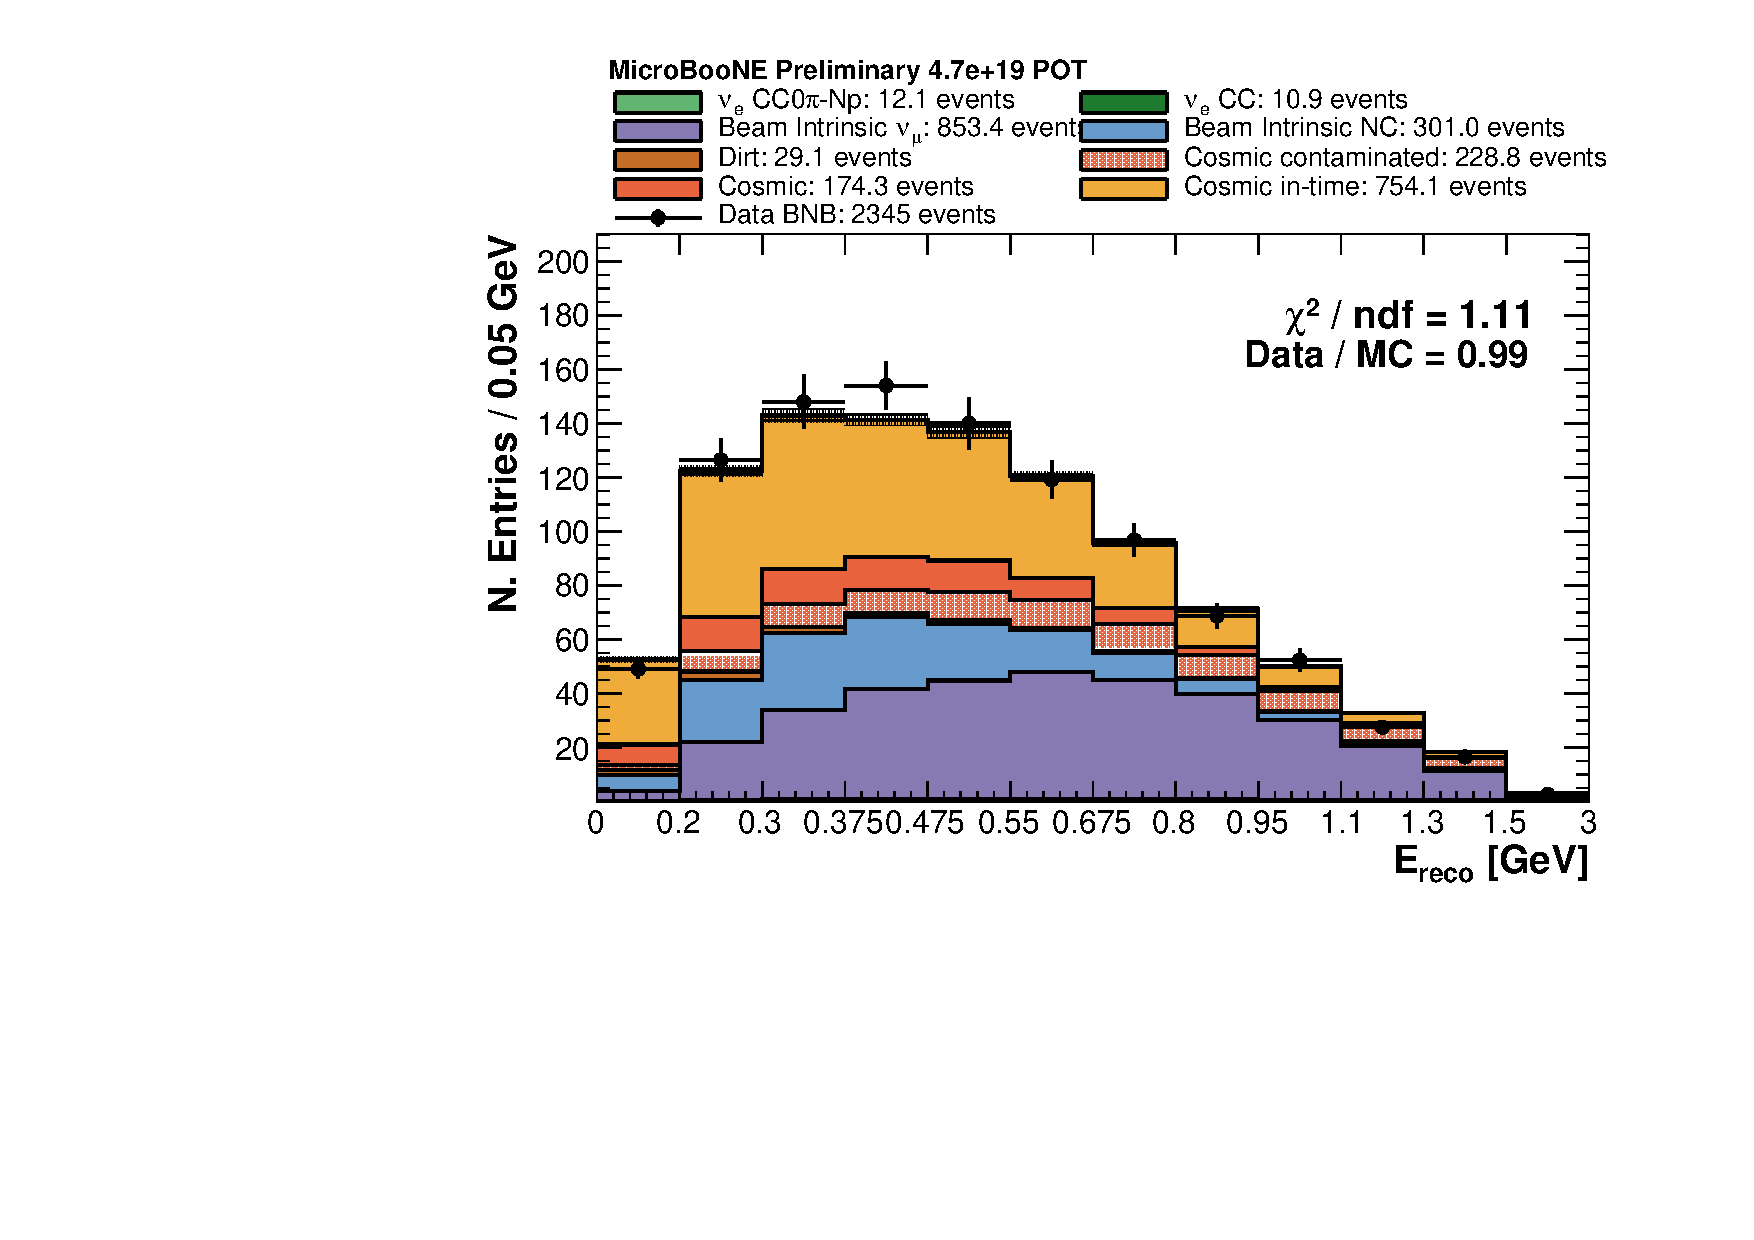
\includegraphics[width=0.65\linewidth]{figures/h_fixed_energy.pdf}
  \caption{Reconstructed energy spectrum after the event selection algorithm and the veto of the events selected by the \texttt{UBXSec} module. The histograms of the event categories are stacked.}
  \label{fig:spectrum}
\end{figure}

Figure \ref{fig:thetaphi} shows the angular distributions of the most energetic shower-like object for data and Monte Carlo. The inclination angle $\theta$ distribution agrees well both for shape and normalization. The azimuthal angle $\phi$ distribution shows a slight disagreement around $\phi = 0^{\circ}$ and $\phi = \pm180^{\circ}$.

\begin{figure}[htbp]
\centering
  \begin{subfigure}{0.45\textwidth}
    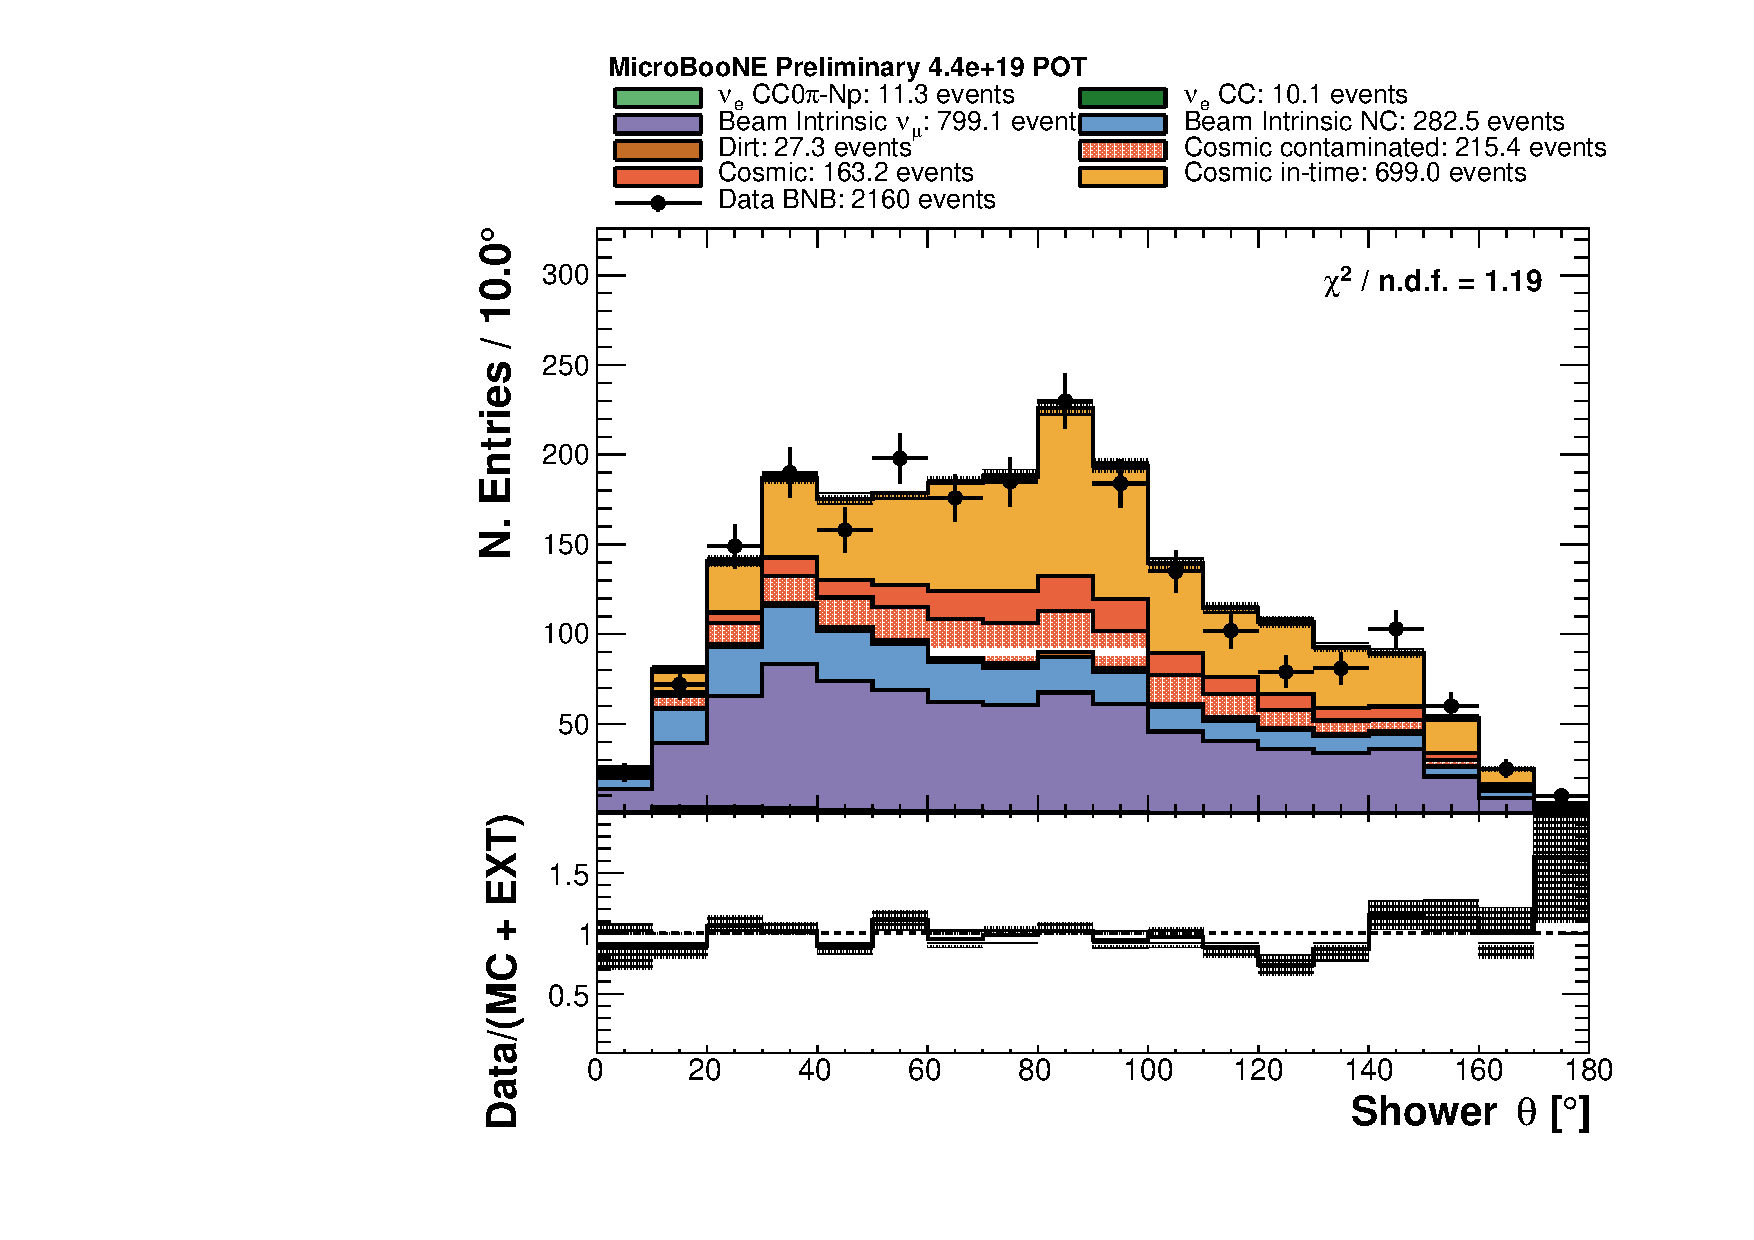
\includegraphics[width=\linewidth]{figures/h_shower_theta.pdf}
    \caption{Inclination angle $\theta$.} 
  \end{subfigure}
    \begin{subfigure}{0.45\textwidth}
    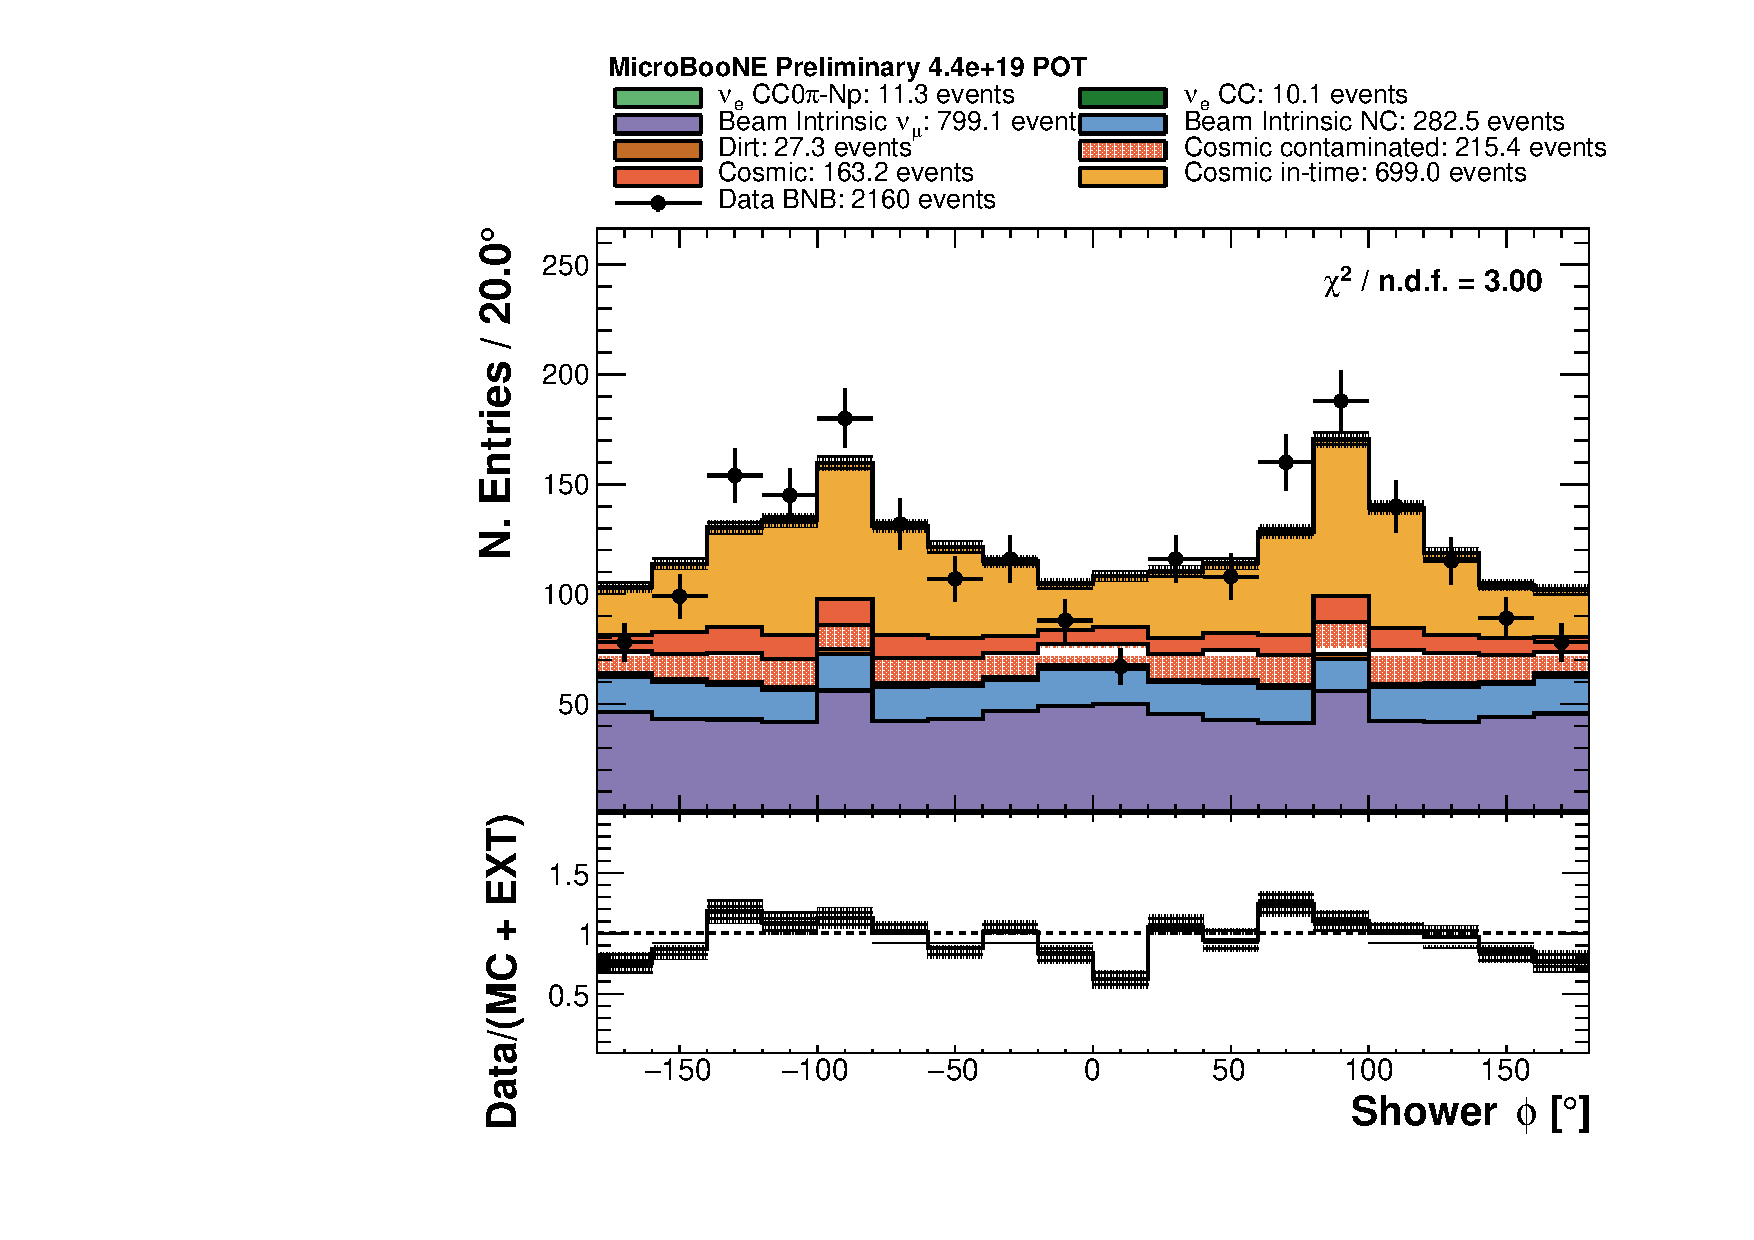
\includegraphics[width=\linewidth]{figures/h_shower_phi.pdf}
    \caption{Azimuthal angle $\phi$.} 
  \end{subfigure}
  \caption{Distribution of the azimuthal angle $\phi$ and the inclination angle $\theta$ of the most energetic shower after the CC \texorpdfstring{$\nu_{\mu}$}{numu} event rejection stage.}\label{fig:thetaphi}
\end{figure}



\subsection{Track-like/Shower-like object reclassification}\label{sec:reclass}
\subsubsection{Classifier disagreement}
An object reconstructed by the Pandora framework in the TPC can be of two distinct types: track-like or shower-like. This assignment is performed directly by the Pandora framework using a Support Vector Machine. However, the scope of the framework is very broad and the object classification is not optimized on our topology. 
The classifier is trained on simulated events, using information from all the three wire planes and its performances are proportional to the number of reconstructed hits. As such, even a slight disagreement between the detector behavior and its simulation in any of the wire planes can have a strong impact on the classification of track-like or shower-like objects. 
Since our analysis heavily relies on the category of the reconstructed objects in its topology pre-selection, a good agreement between the classifier performances in data and Monte Carlo is essential.
Moreover, the energy reconstruction procedure is different for track-like and shower-like objects, as described in Section \ref{sec:energyreco}: an eventual classification disagreement will directly cause a disagreement in the reconstructed energy spectrum.


\begin{figure}[htbp]
\centering
  \begin{subfigure}{0.45\textwidth}
    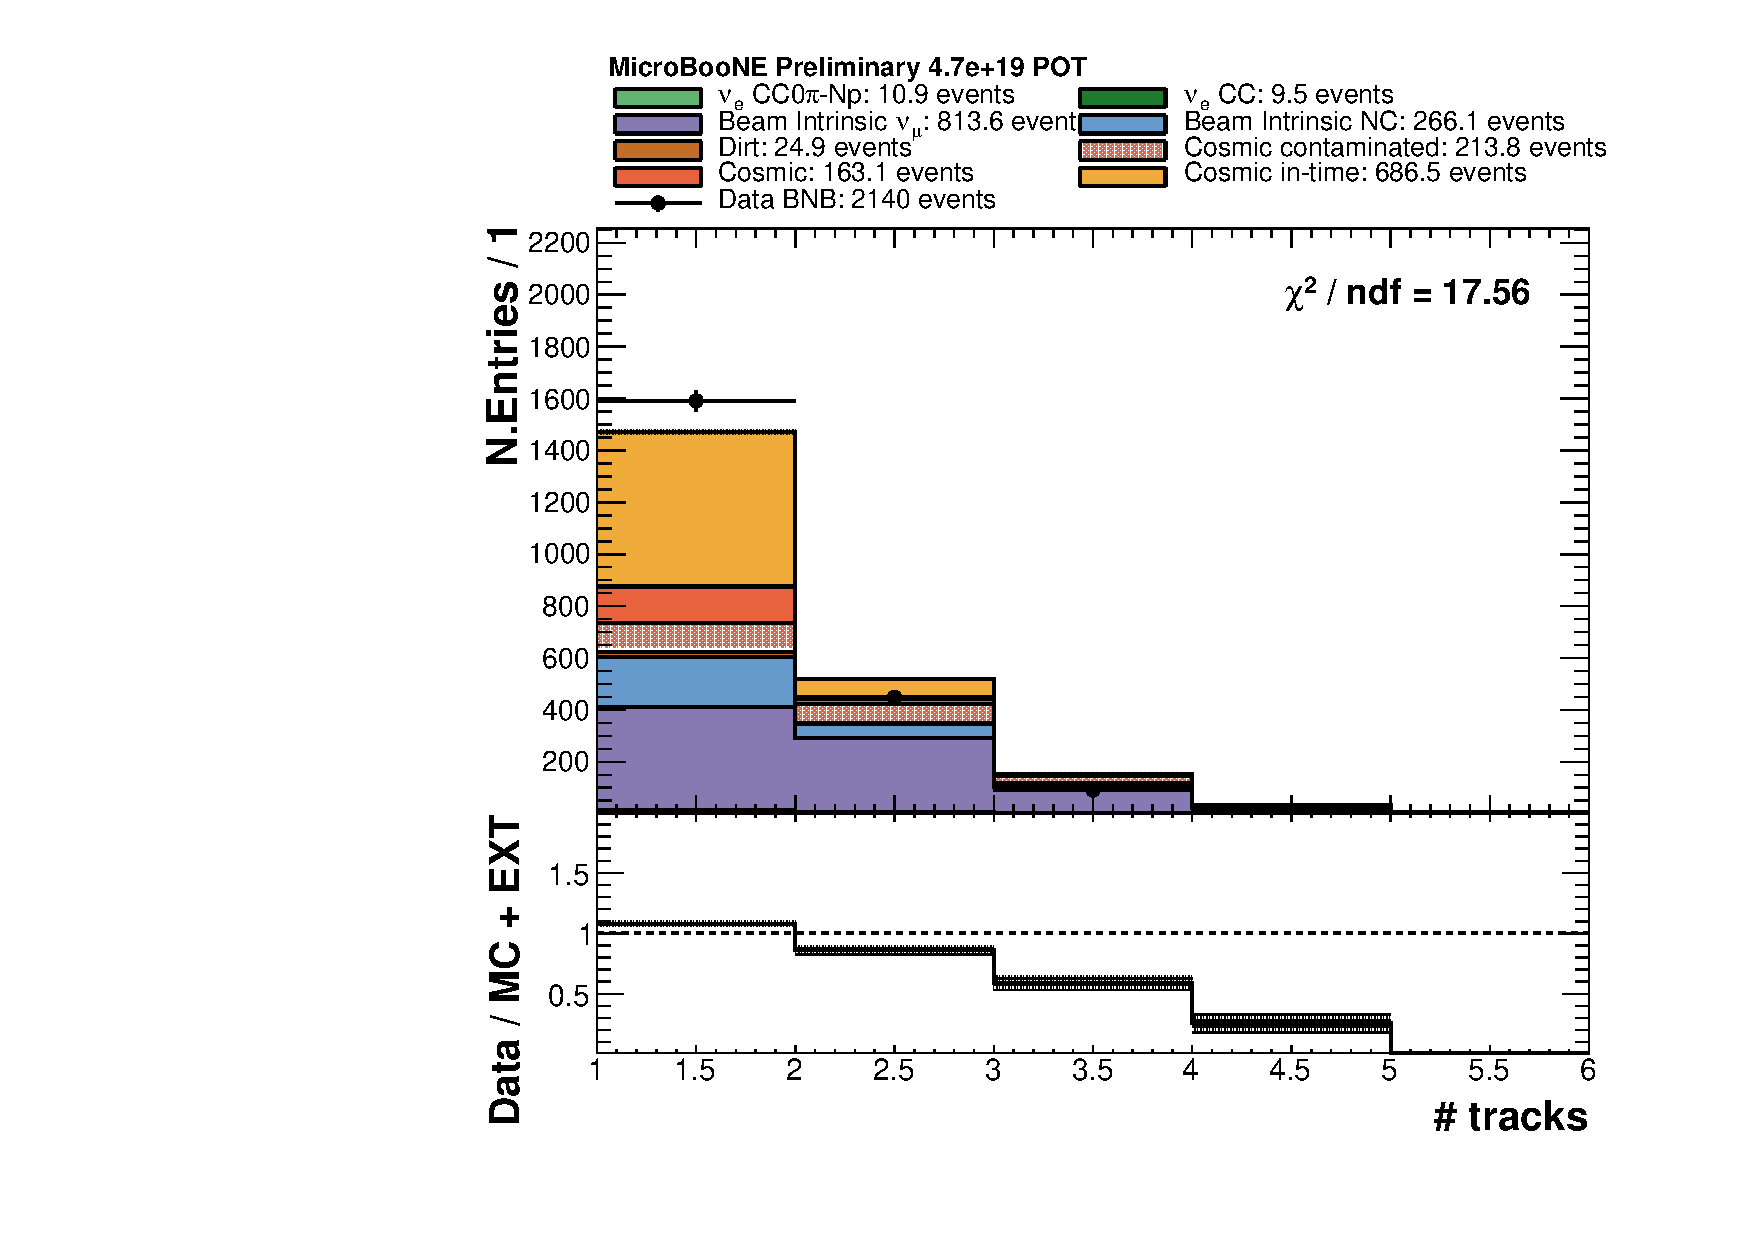
\includegraphics[width=\linewidth]{figures/h_n_tracks_before.pdf}
    \caption{Number of tracks.} 
  \end{subfigure}
    \begin{subfigure}{0.45\textwidth}
    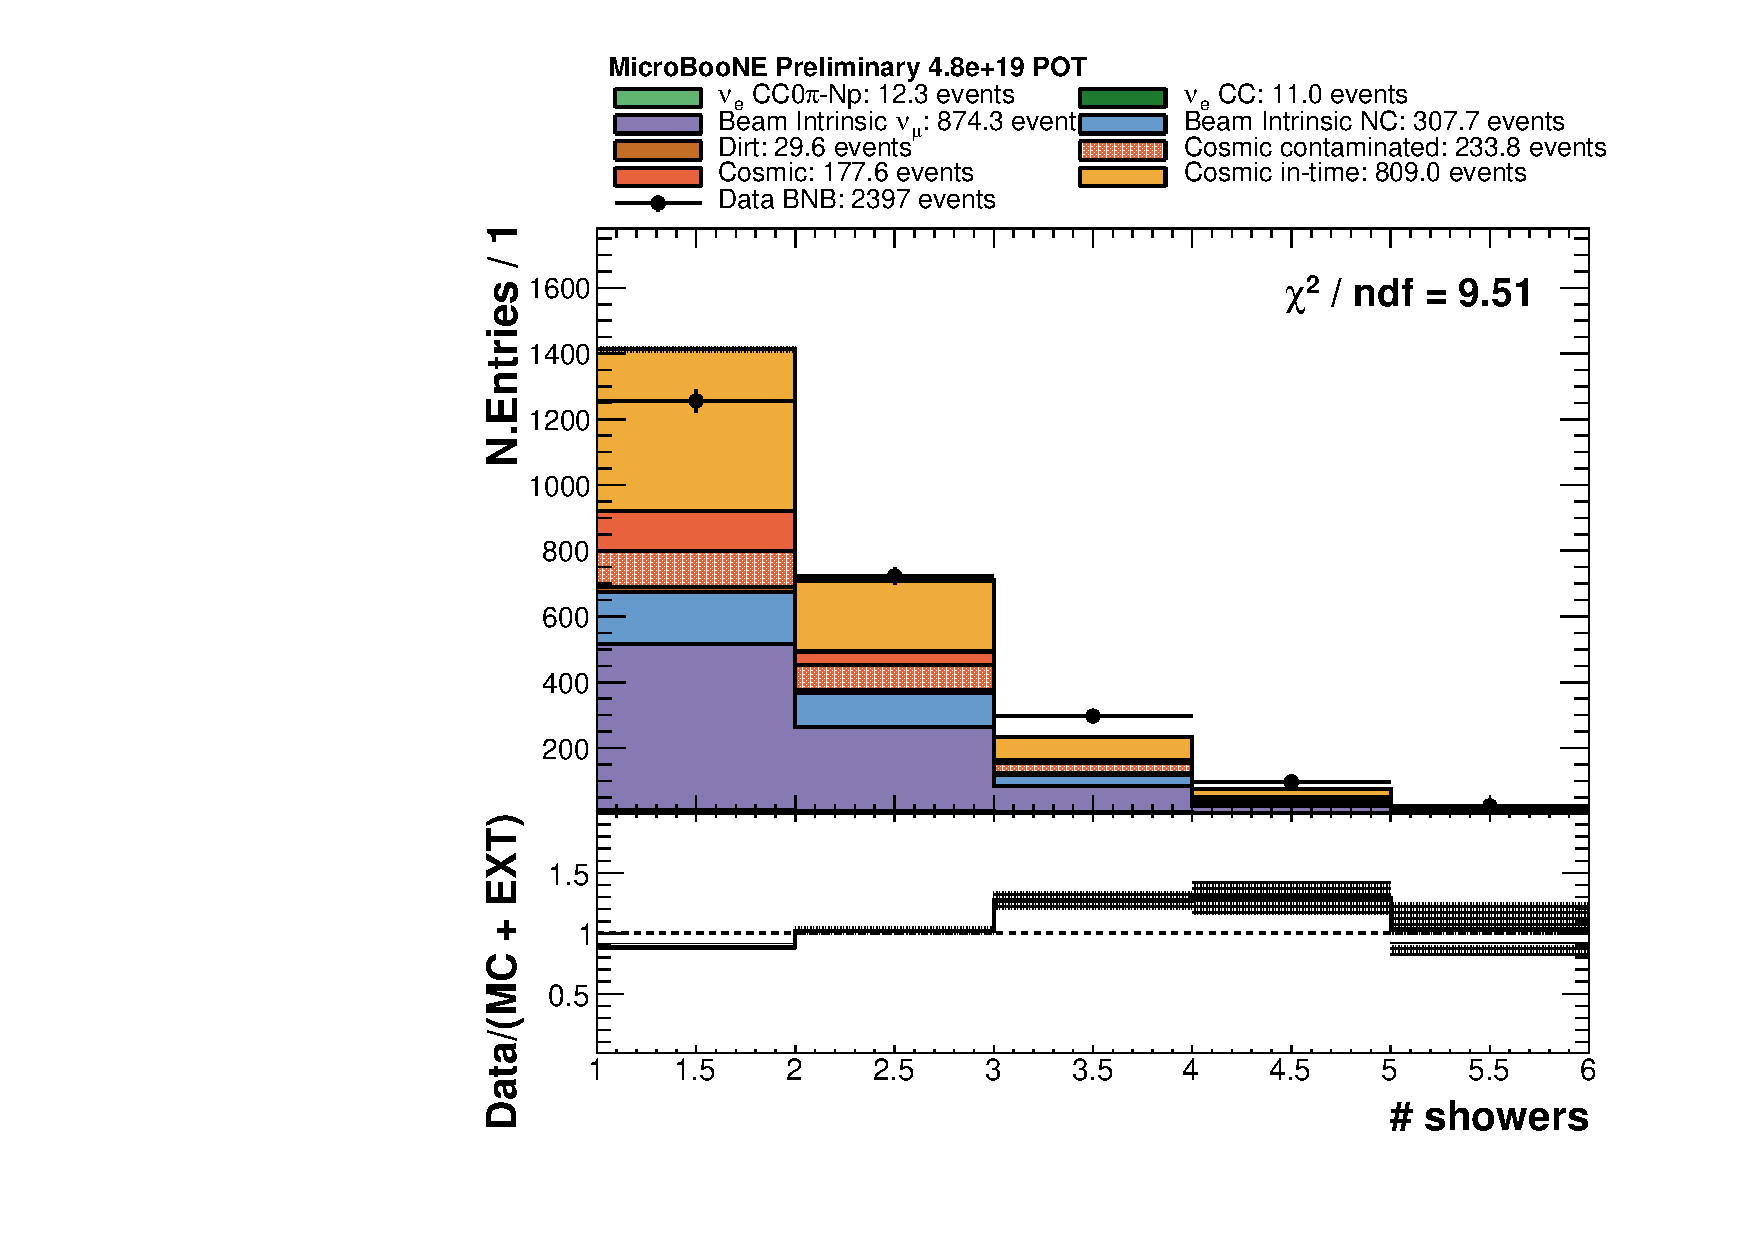
\includegraphics[width=\linewidth]{figures/h_n_showers_before.pdf}
    \caption{Number of showers.} 
  \end{subfigure}
  \caption{Number of tracks and number of showers per event before the reclassification procedure.}\label{fig:nshowers}
\end{figure}

The distributions of the number of track-like objects and of the number of shower-like objects in a selected event hint at a tendency of the classifier to select an object as shower-like more often in the data than in the simulation.

\begin{figure}[htbp]
\centering
  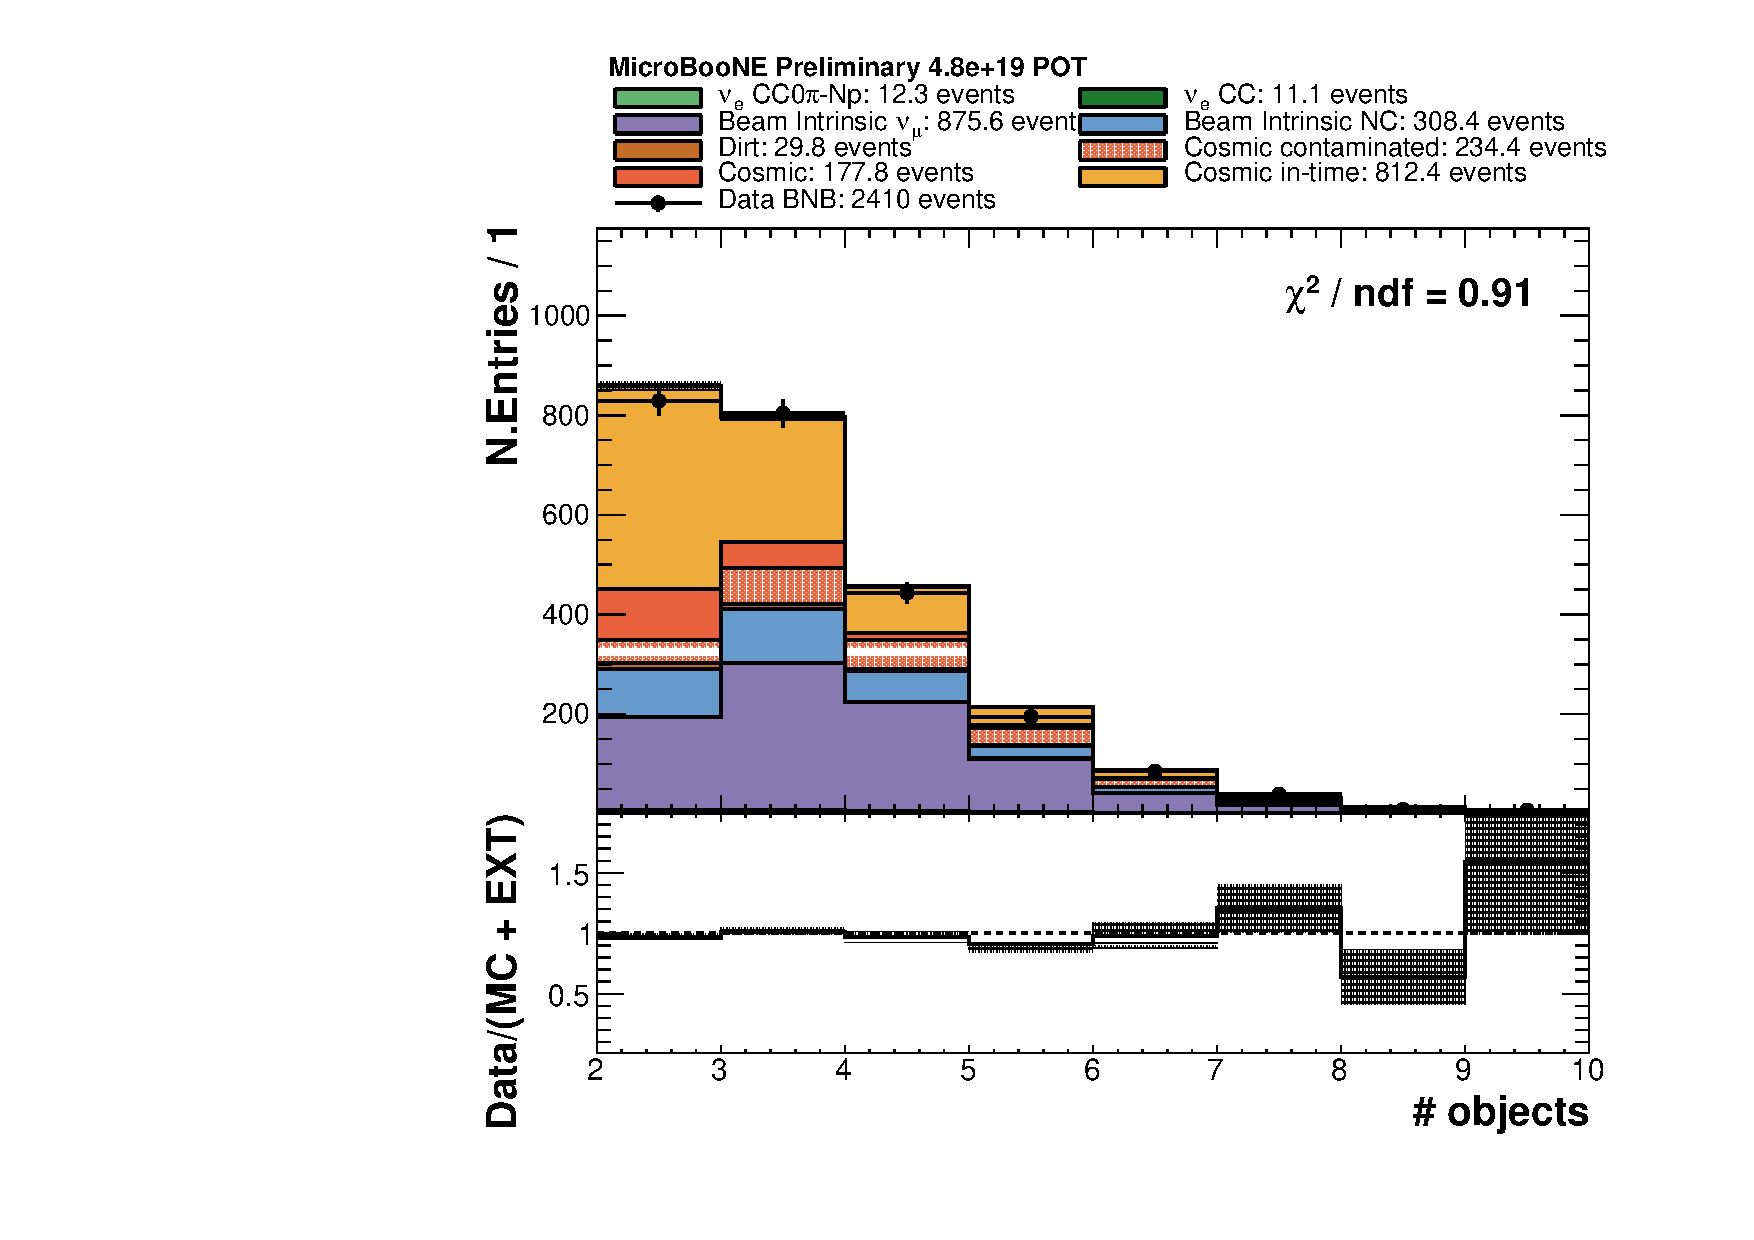
\includegraphics[width=0.65\linewidth]{figures/h_n_objects.pdf}
  \caption{Distribution of the total number of reconstructed objects per event.}
  \label{fig:nobjects}
\end{figure}

Figure \ref{fig:nshowers} shows the number of showers and the number of tracks per event in our selected sample after the optical and topological pre-selection. The ratio plot clearly indicates the presence of a bias: there are more events with a high number of reconstructed showers and more events with a low number of reconstructed tracks in the data than in the Monte Carlo. 

The distribution of the total number of reconstructed objects in Figure \ref{fig:nobjects} (regardless of their category) shows instead a very good agreement and no bias.


The simulation does not perfectly reflects the detector status: in particular, we measured the hit residuals of the track-like objects in the collection plane, defined as the distance between the reconstructed hit position in two dimensions (wire, time) and the reconstructed track trajectory. Figure \ref{fig:res} shows that the distribution of the mean of the residuals is peaked around zero as expected, both for data and Monte Carlo, while the standard deviation in the data is shifted towards higher values. 

\begin{figure}[htbp]
\centering
  \begin{subfigure}{0.45\textwidth}
    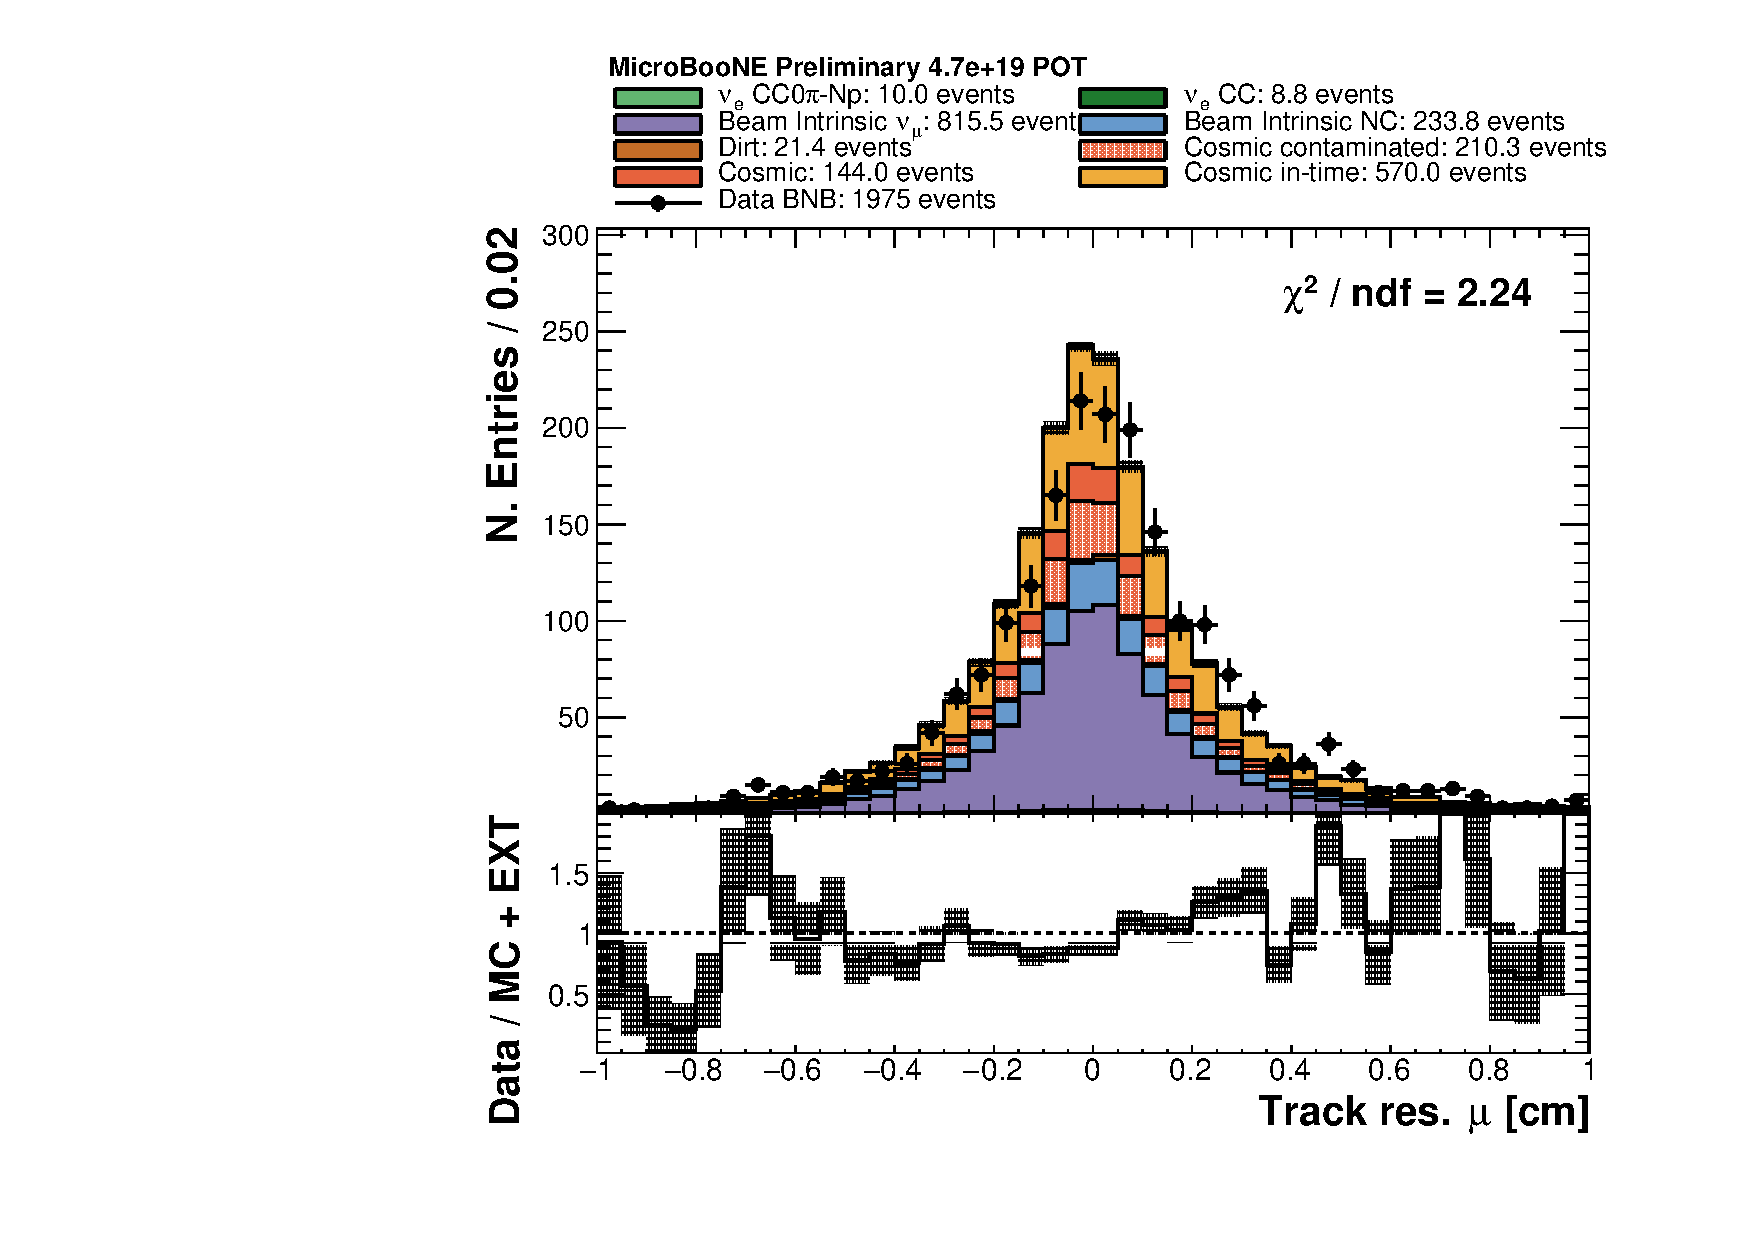
\includegraphics[width=\linewidth]{figures/h_track_res_mean.pdf}
    \caption{Track residual mean.} 
  \end{subfigure}
    \begin{subfigure}{0.45\textwidth}
    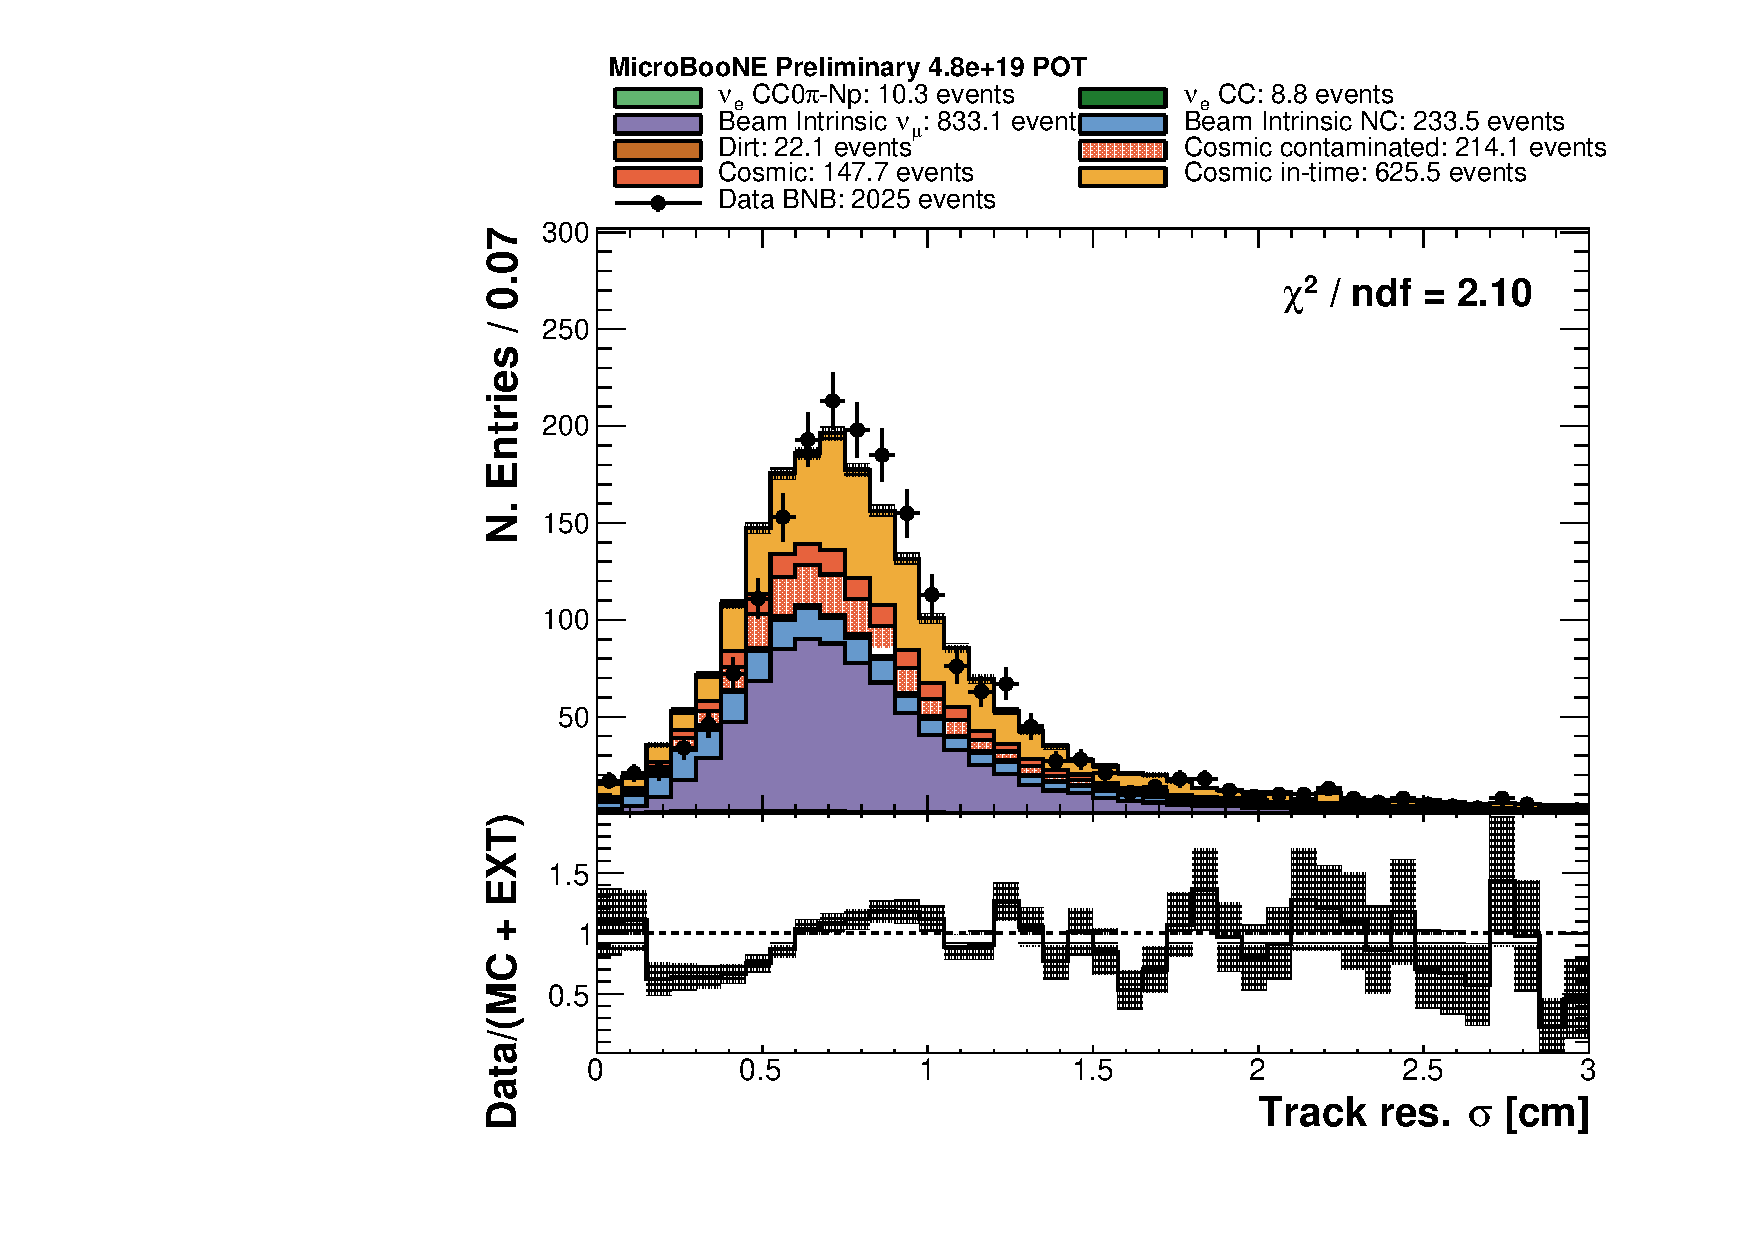
\includegraphics[width=\linewidth]{figures/h_track_res_std.pdf}
    \caption{Track residual standard deviation.} 
  \end{subfigure}
  \caption{Distribution of the mean and of the standard deviation of the track residuals.}\label{fig:res}
\end{figure}

The distribution of the principal component eigenvalue for track-like objects and shower-like objects also shows a disagreement: the data distributions are broader and the ratios have a decreasing slope, especially for high values (Figure \ref{fig:pca}).

\begin{figure}[htbp]
\centering
  \begin{subfigure}{0.45\textwidth}
    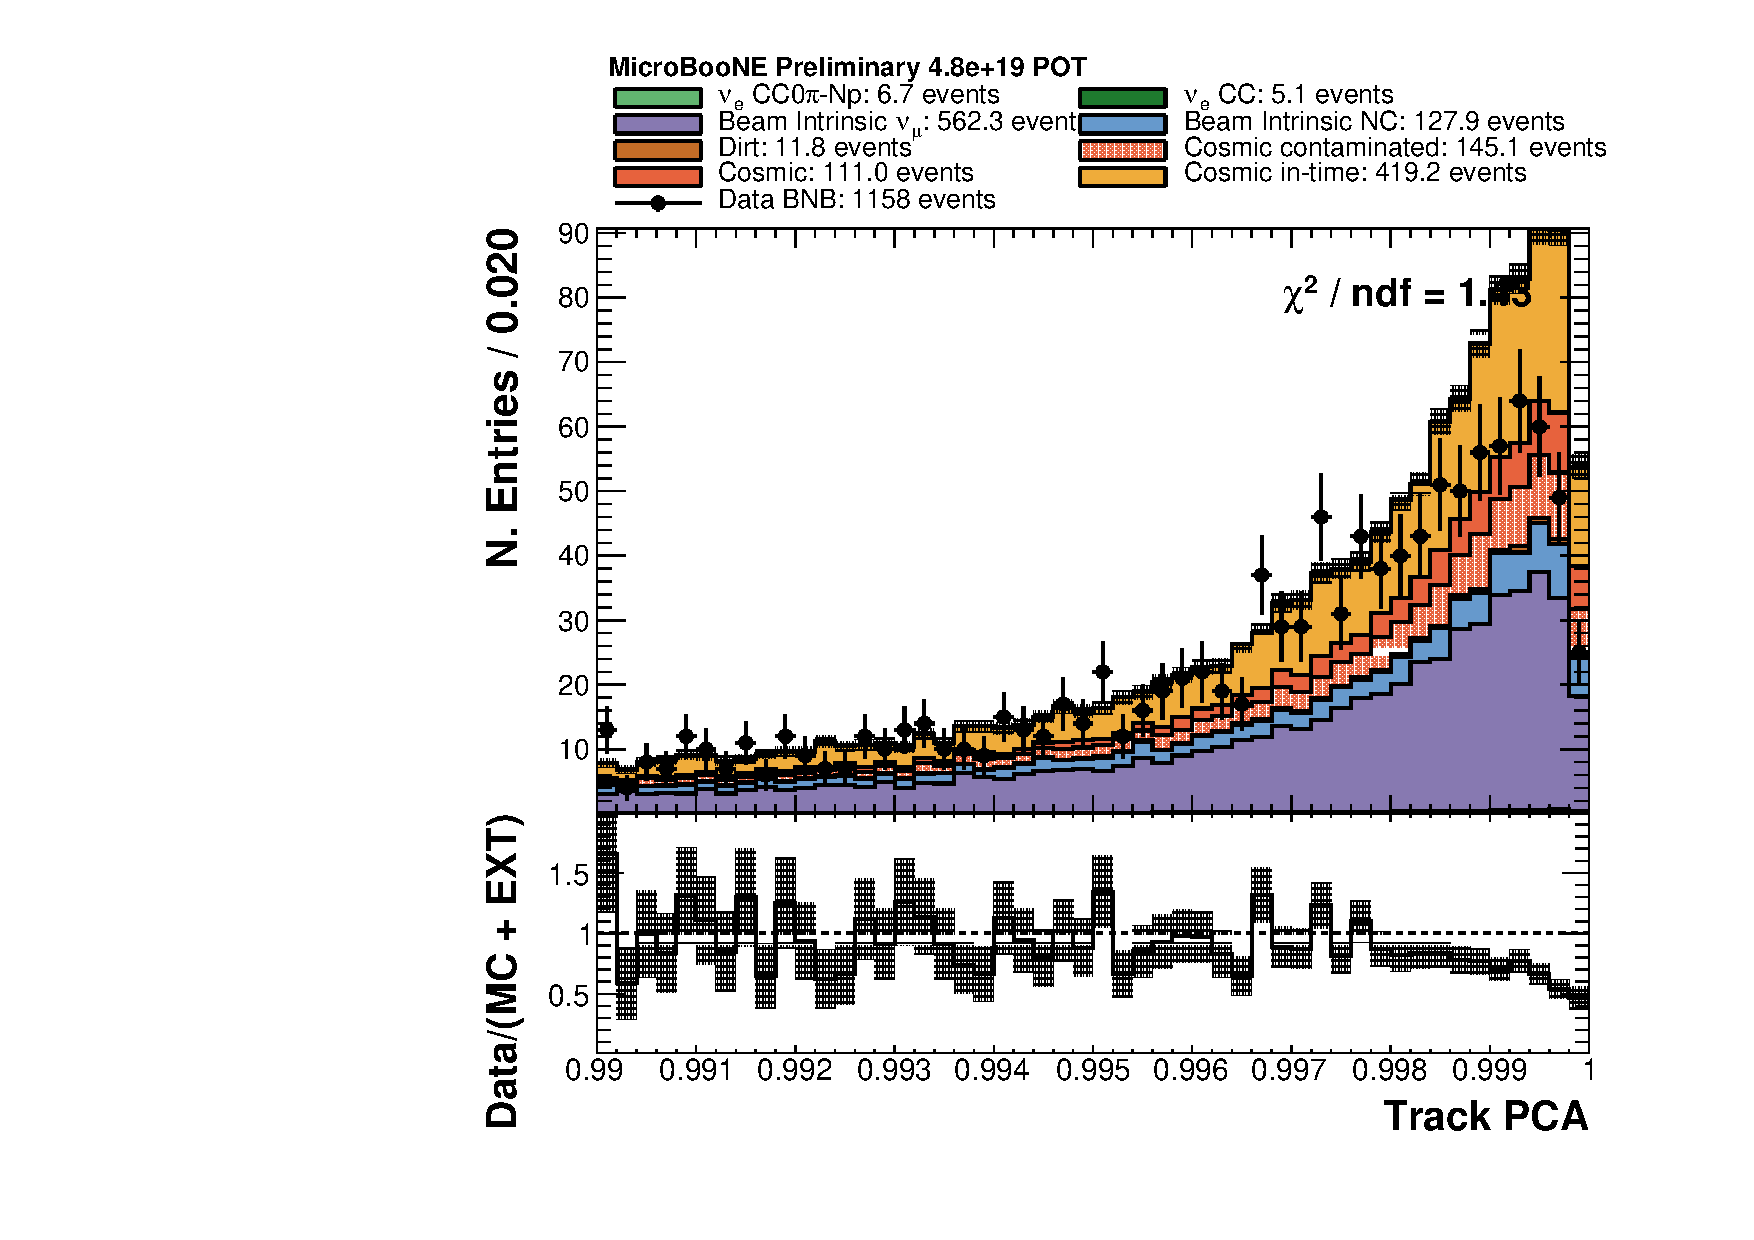
\includegraphics[width=\linewidth]{figures/h_track_pca.pdf}
    \caption{Track PCA eigenvalue.} 
  \end{subfigure}
    \begin{subfigure}{0.45\textwidth}
    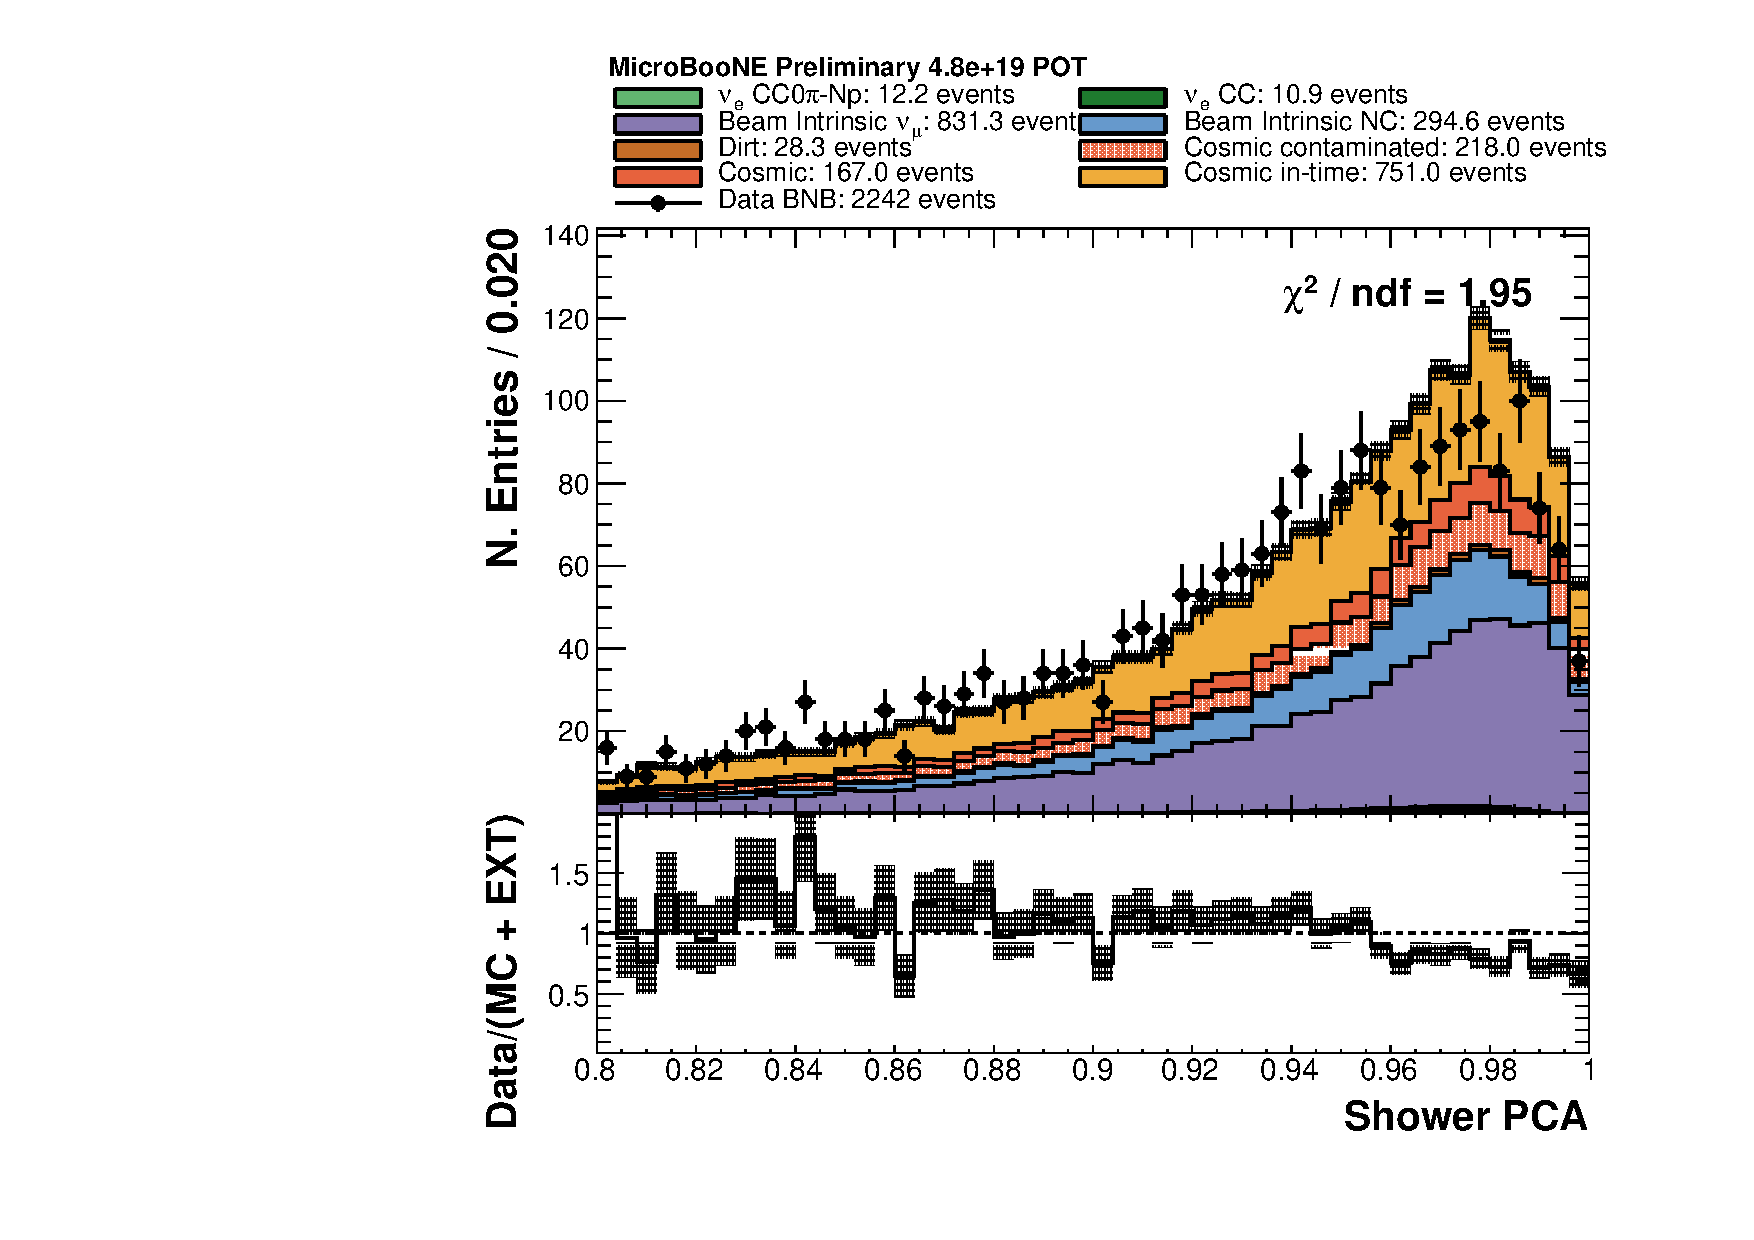
\includegraphics[width=\linewidth]{figures/h_shower_pca.pdf}
    \caption{Shower PCA eigenvalue.} 
  \end{subfigure}
  \caption{Principal Component first eigenvalue for reconstructed tracks and reconstructed showers.}\label{fig:pca}
\end{figure}

This evidence points towards a detector mis-modeling in the simulation: Figure \ref{fig:evdpandora} shows the Pandora data event display in one of the induction plane of a track objects that was reconstructed as a shower-like object. The presence of noise hits around the track created artifacts that induced the SVM to classify the object as a shower.

\begin{figure}[htbp]
\centering
  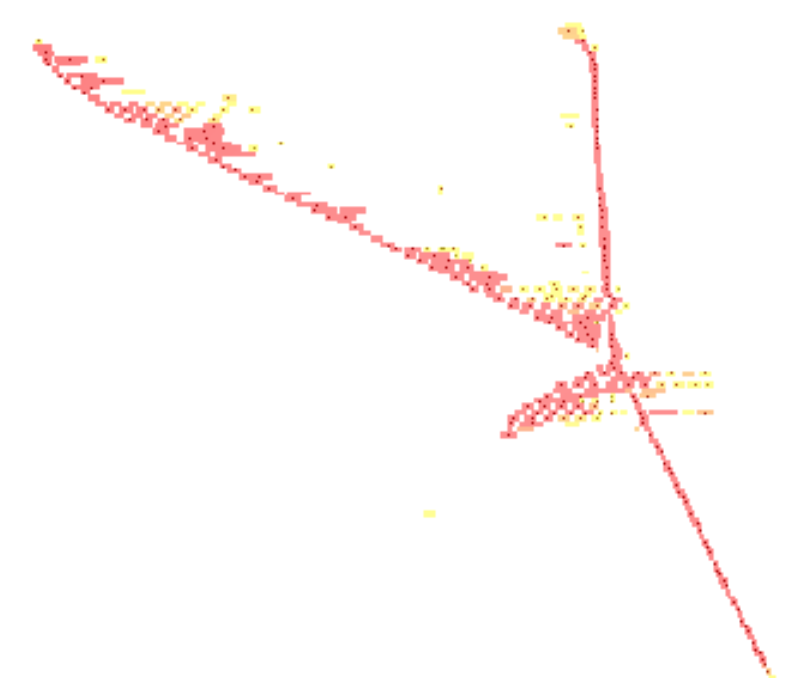
\includegraphics[width=0.45\linewidth]{figures/pandora.png}
  \caption{Pandora data event display in one of the induction plane of a track objects that was reconstructed as a shower-like object.}
  \label{fig:evdpandora}
\end{figure}

\subsubsection{Reclassification procedure}
In order to solve this discrepancy it is possible to reclassify the reconstructed objects exploiting the particular topology of our signal events. In particular, a well-reconstructed $\nu_{e}$ CC0$\pi$-Np event will have a reconstructed shower corresponding to the electron and N reconstructed tracks, where N is the number of protons above detection threshold. 

The Pandora reconstruction framework can split the electromagnetic shower in two or more objects: however, even if distinct, the showers will have in general a low angular separation. A small reconstructed shower-like object with a high angular separation from the most energetic one has a high probability to be in reality a mis-reconstructed proton track. Thus, we reclassify the shower-like objects based on the angular separation between each small shower-like object and the most-energetic shower: if the angle is larger than $15^{\circ}$, the shower-like object is reclassified as a track-like object.

Figure \ref{fig:showerangle} shows the proton reconstruction efficiency and purity as a function of the angular reclassification cut. The efficiency here is defined as the ratio between the number of protons in the final state above threshold and the number of proton-associated reconstructed tracks. The purity is defined as the ration between the number of proton-associated reconstructed tracks and the total number of reconstructed tracks. These two quantities have been measured in a sample of $\nu_{e}$ CC0$\pi$-Np events that pass our selection algorithm.  The $15^{\circ}$ threshold is chosen because it maximizes the efficiency while keeping a reasonable reconstruction purity (above 70\%).

\begin{figure}[htbp]
\centering
  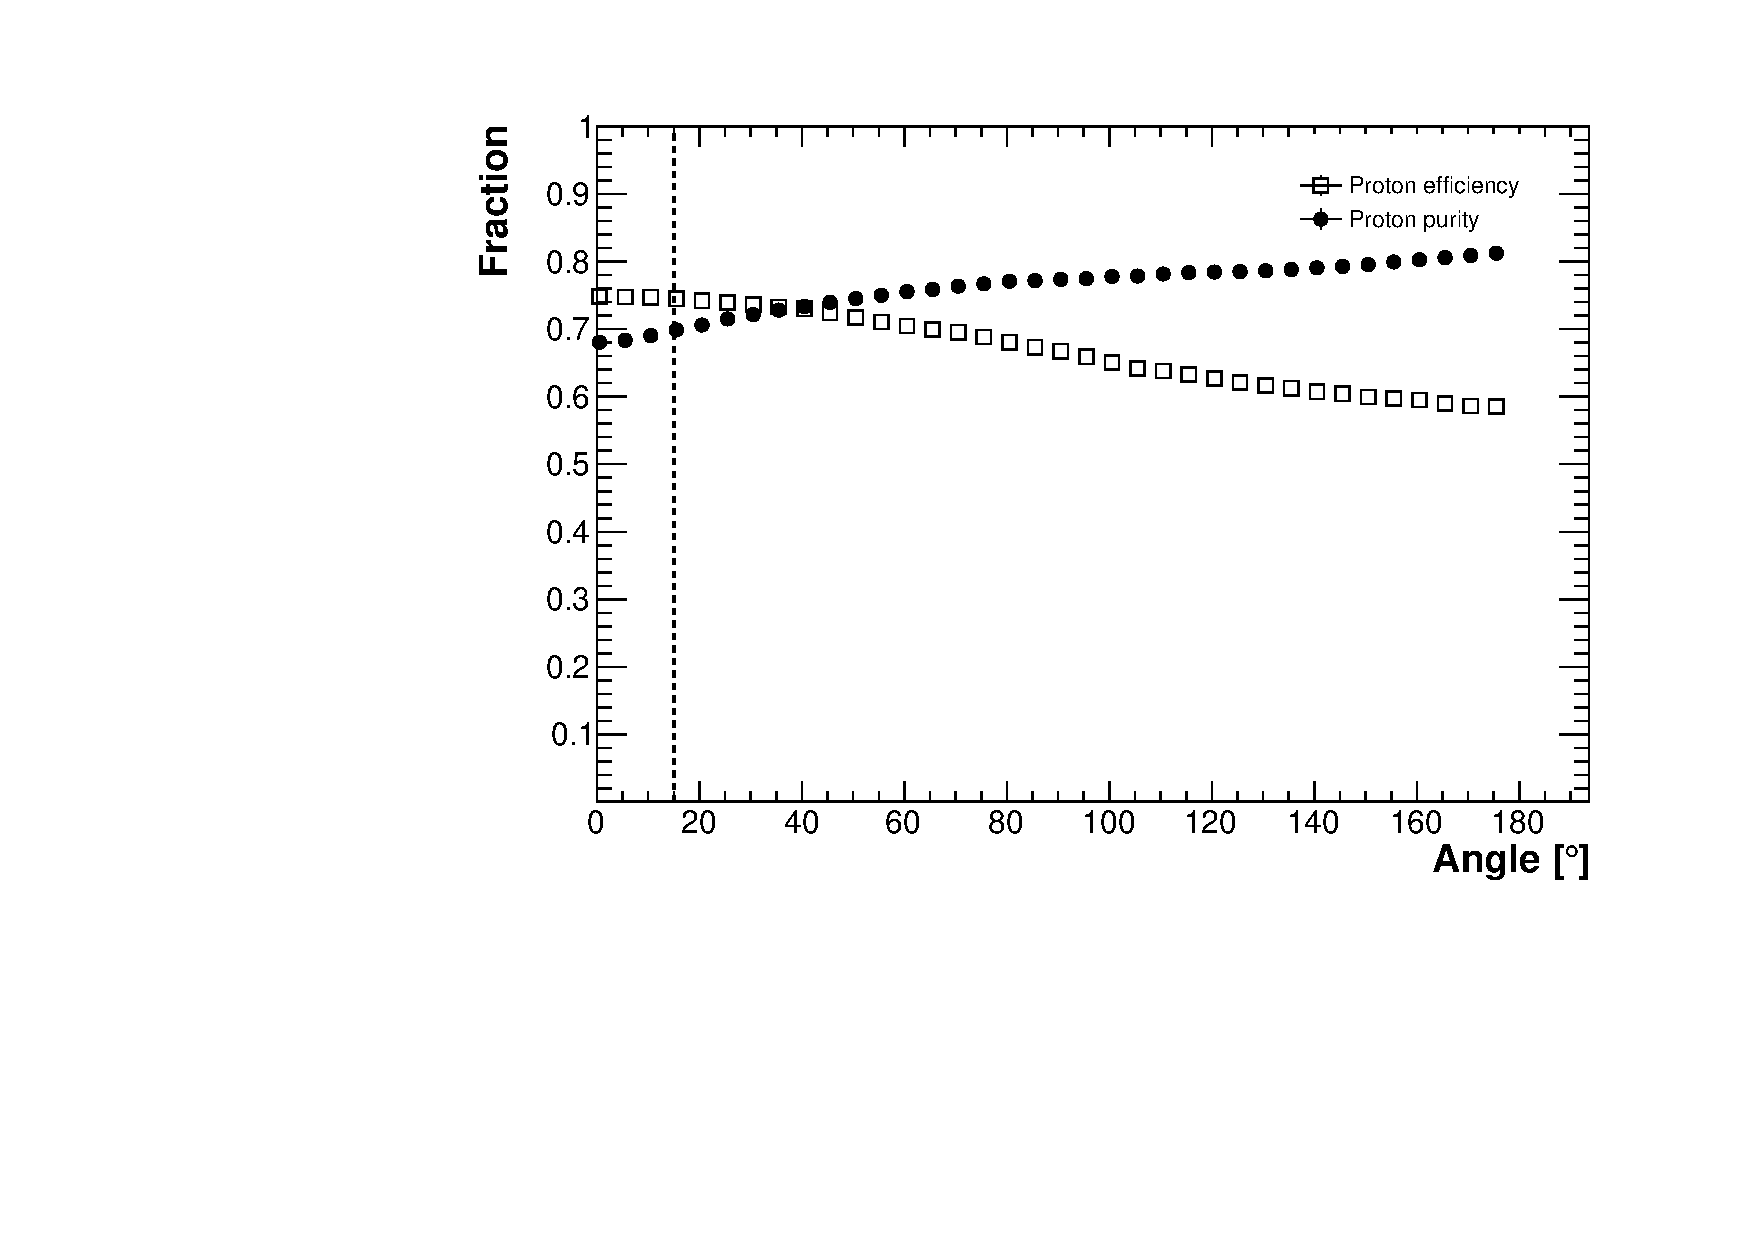
\includegraphics[width=0.65\linewidth]{figures/proton_angle.pdf}
  \caption{Proton reconstruction efficiency and purity as a function of the angular separation reclassification threshold.}
  \label{fig:showerangle}
\end{figure}

It is also possible for a small electron shower remnant to be reconstructed as a track-like object. Thus, we reclassify a track-like object as a shower if it is within the cone of the most energetic shower. This criterion correctly identifies a shower remnant in the 98.9\% of the cases.

\begin{figure}[htbp]
\centering
  \begin{subfigure}{0.45\textwidth}
    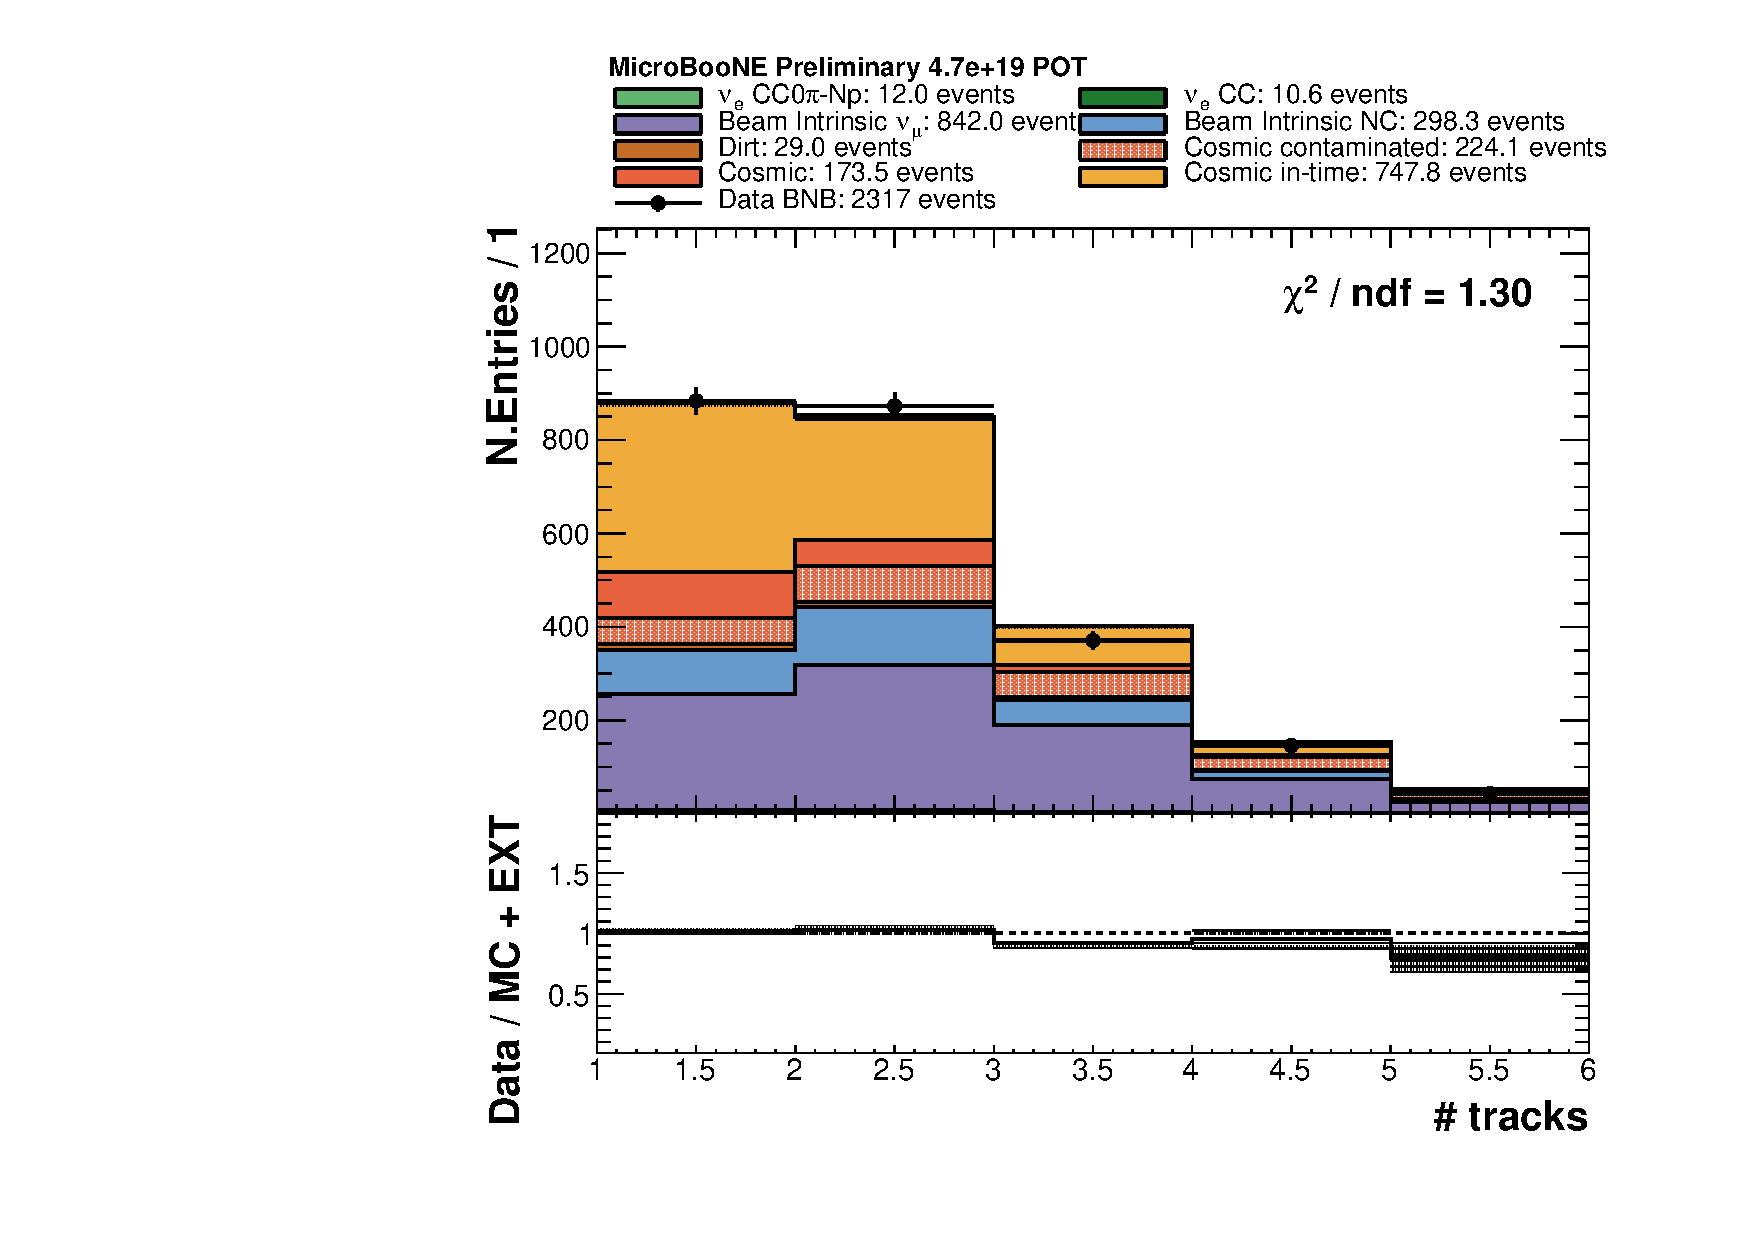
\includegraphics[width=\linewidth]{figures/h_n_tracks.pdf}
    \caption{Number of tracks.} 
  \end{subfigure}
    \begin{subfigure}{0.45\textwidth}
    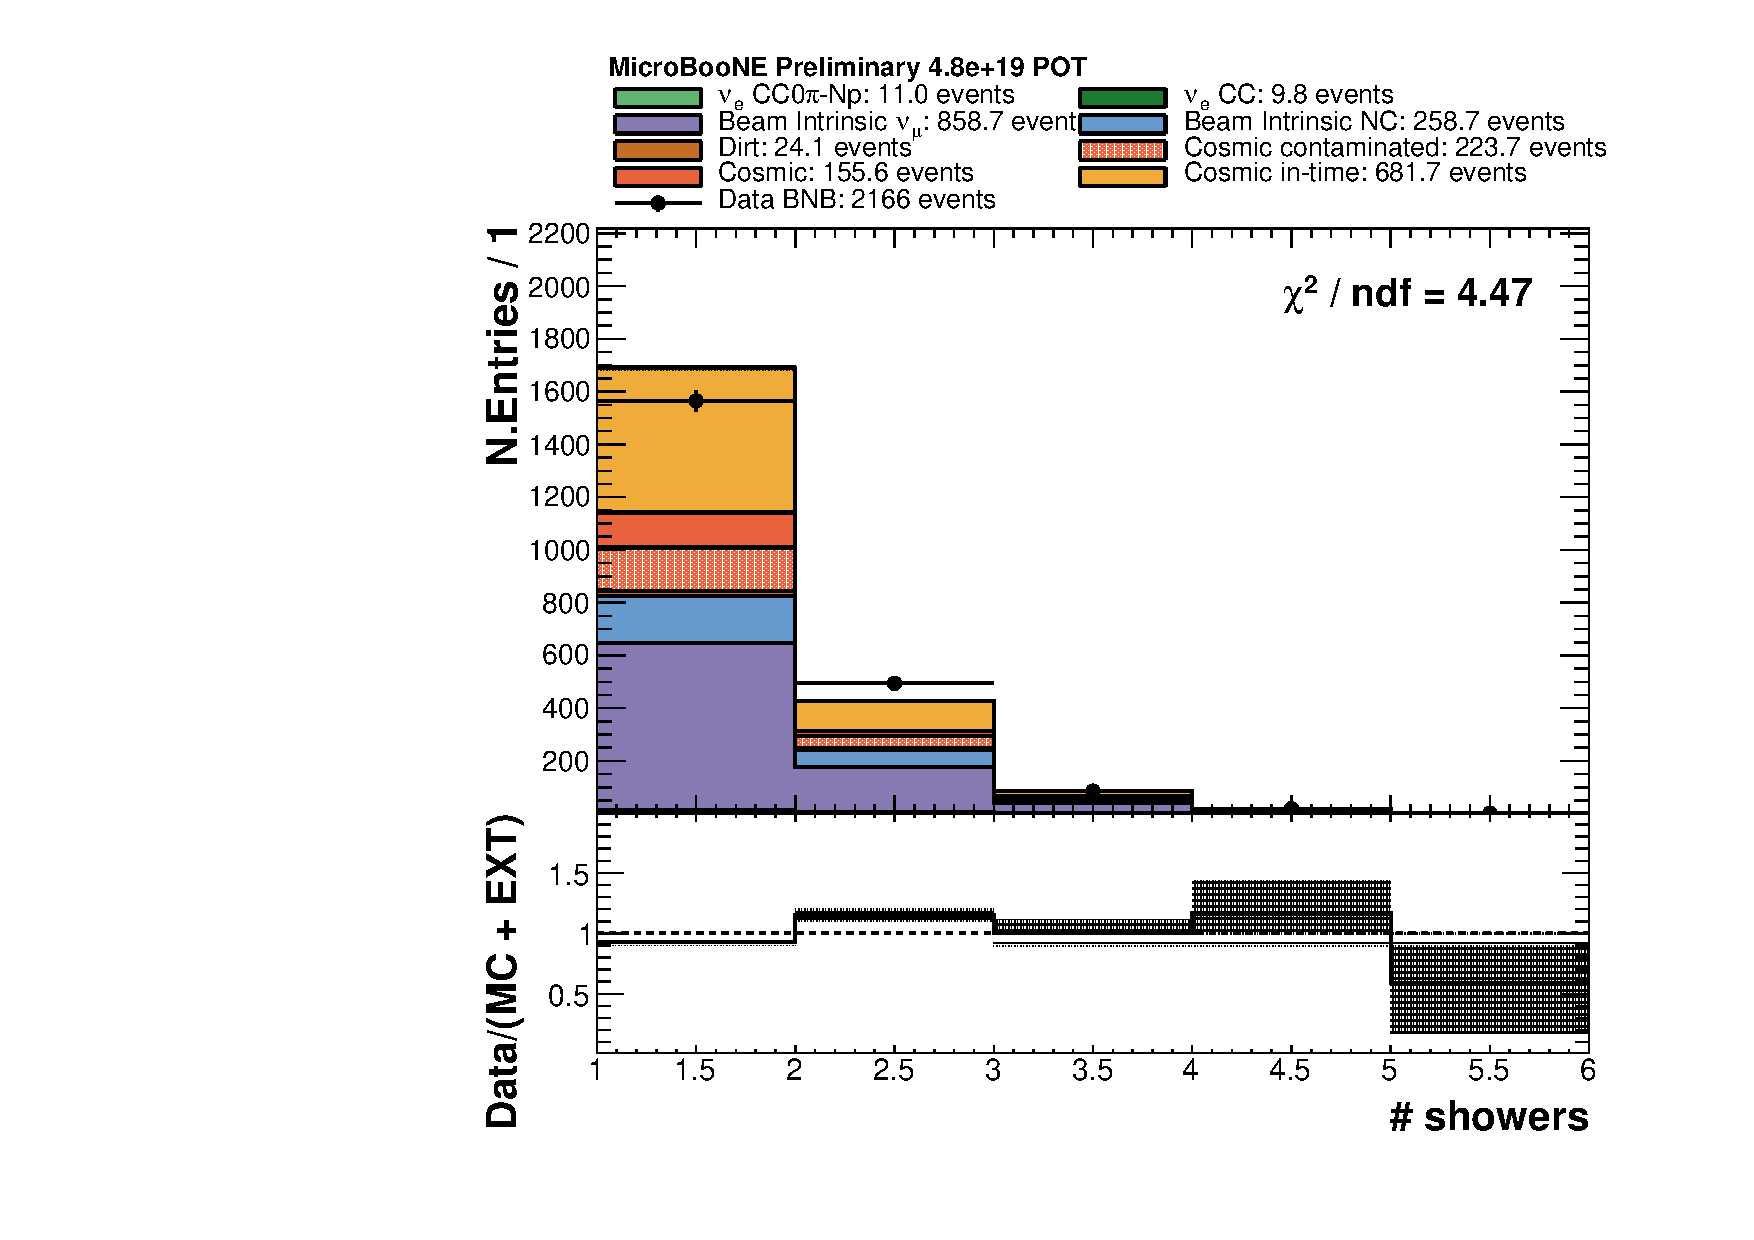
\includegraphics[width=\linewidth]{figures/h_n_showers.pdf}
    \caption{Number of showers.} 
  \end{subfigure}
  \caption{Number of tracks and number of showers per event after the reclassification procedure.}\label{fig:nshowers_after}
\end{figure}

Figure \ref{fig:nshowers_after} shows the number of shower-like objects and the number of track-like objects per event after these two reclassification procedures. The agreement improves and the bias in the ratio disappears. 

\subsection{Background Rejection}\label{sec:bkg}
\subsubsection{Introduction}
In this section we will describe the cuts applied to our selected sample, in order to isolate the $\nu_{e}$ CC$0\pi$-Np event candidates. The cuts have been chosen to (1) reduce the background, and (2) ensure that the selected events are well reconstructed. The values of each cut have been chosen manually. It would have been possible, in theory, to calculate an optimal set of cuts, maximized by the significance of the $\nu_{e}$ CC0$\pi$-Np events. However, this set of cuts would not have allowed a correct validation of the final selected sample, due to the limited size of the data unblinded sample. As such, the chosen cuts increase the purity of our sample, but also retain a significant amount ($\approx 20$) of selected data events.

\subsubsection{Shower \texorpdfstring{$dE/dx$}{dE/dx}}\label{sec:dedx}
The rate of energy loss per length ($dE/dx$) for electromagnetic showers is measured with a procedure analogous to the one described in \cite{argoneut}. All the hits of the collection plane within a rectangle of 4~cm along the direction of the shower and 1~cm perpendicular to the shower are collected. Figure \ref{fig:evddedx} shows a Monte Carlo event display with an electron shower and the rectangle used to measure the $dE/dx$.

\begin{figure}[htbp]
\centering
  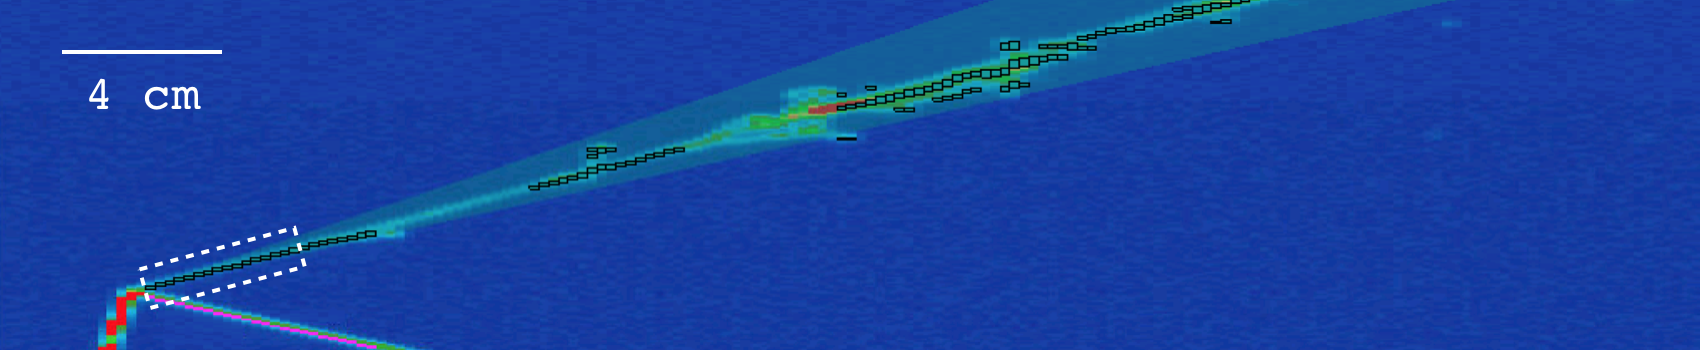
\includegraphics[width=0.9\linewidth]{figures/evddedx.png}
  \caption{Monte Carlo event display of an electron shower in the collection plane with the $1\times4$~cm rectangle used to measure the $dE/dx$. The black boxes correspond to the reconstructed hits.}
  \label{fig:evddedx}
\end{figure}

The $dQ/dx$ for each hit is measured dividing the collected charge ($dQ$) by the pitch ($dx$) between each hit and the next one along the shower direction. The pitch corresponds to the distance in the TPC that a particle travels between its two projections  on adjacent wires, which is \emph{at least} the wire spacing (3~mm for MicroBooNE \cite{detector}). 

The $dE/dx$ is calculated from the $dQ/dx$ by using the calibration factor measured in \eqref{eq:calib}.
Since the distribution of the $dE/dx$ hit values has an asymmetric tail due to the Landau nature of the process, we assign to the shower the median (and not the mean) of the $dE/dx$ hit distribution.

Figure \ref{fig:dedx} shows the $dE/dx$ hit distribution and the $dE/dx$ median distribution for electron and photon showers obtained with a Monte Carlo simulation. In this plot, each shower is required to have at least 10 reconstructed hits. As expected, the electron distribution is peaked around 2~MeV/cm. The photon distribution has two peaks, one around 2~MeV/cm and one around 4~MeV/cm. 


\begin{figure}[htbp]
\centering
  \begin{subfigure}{0.45\textwidth}
    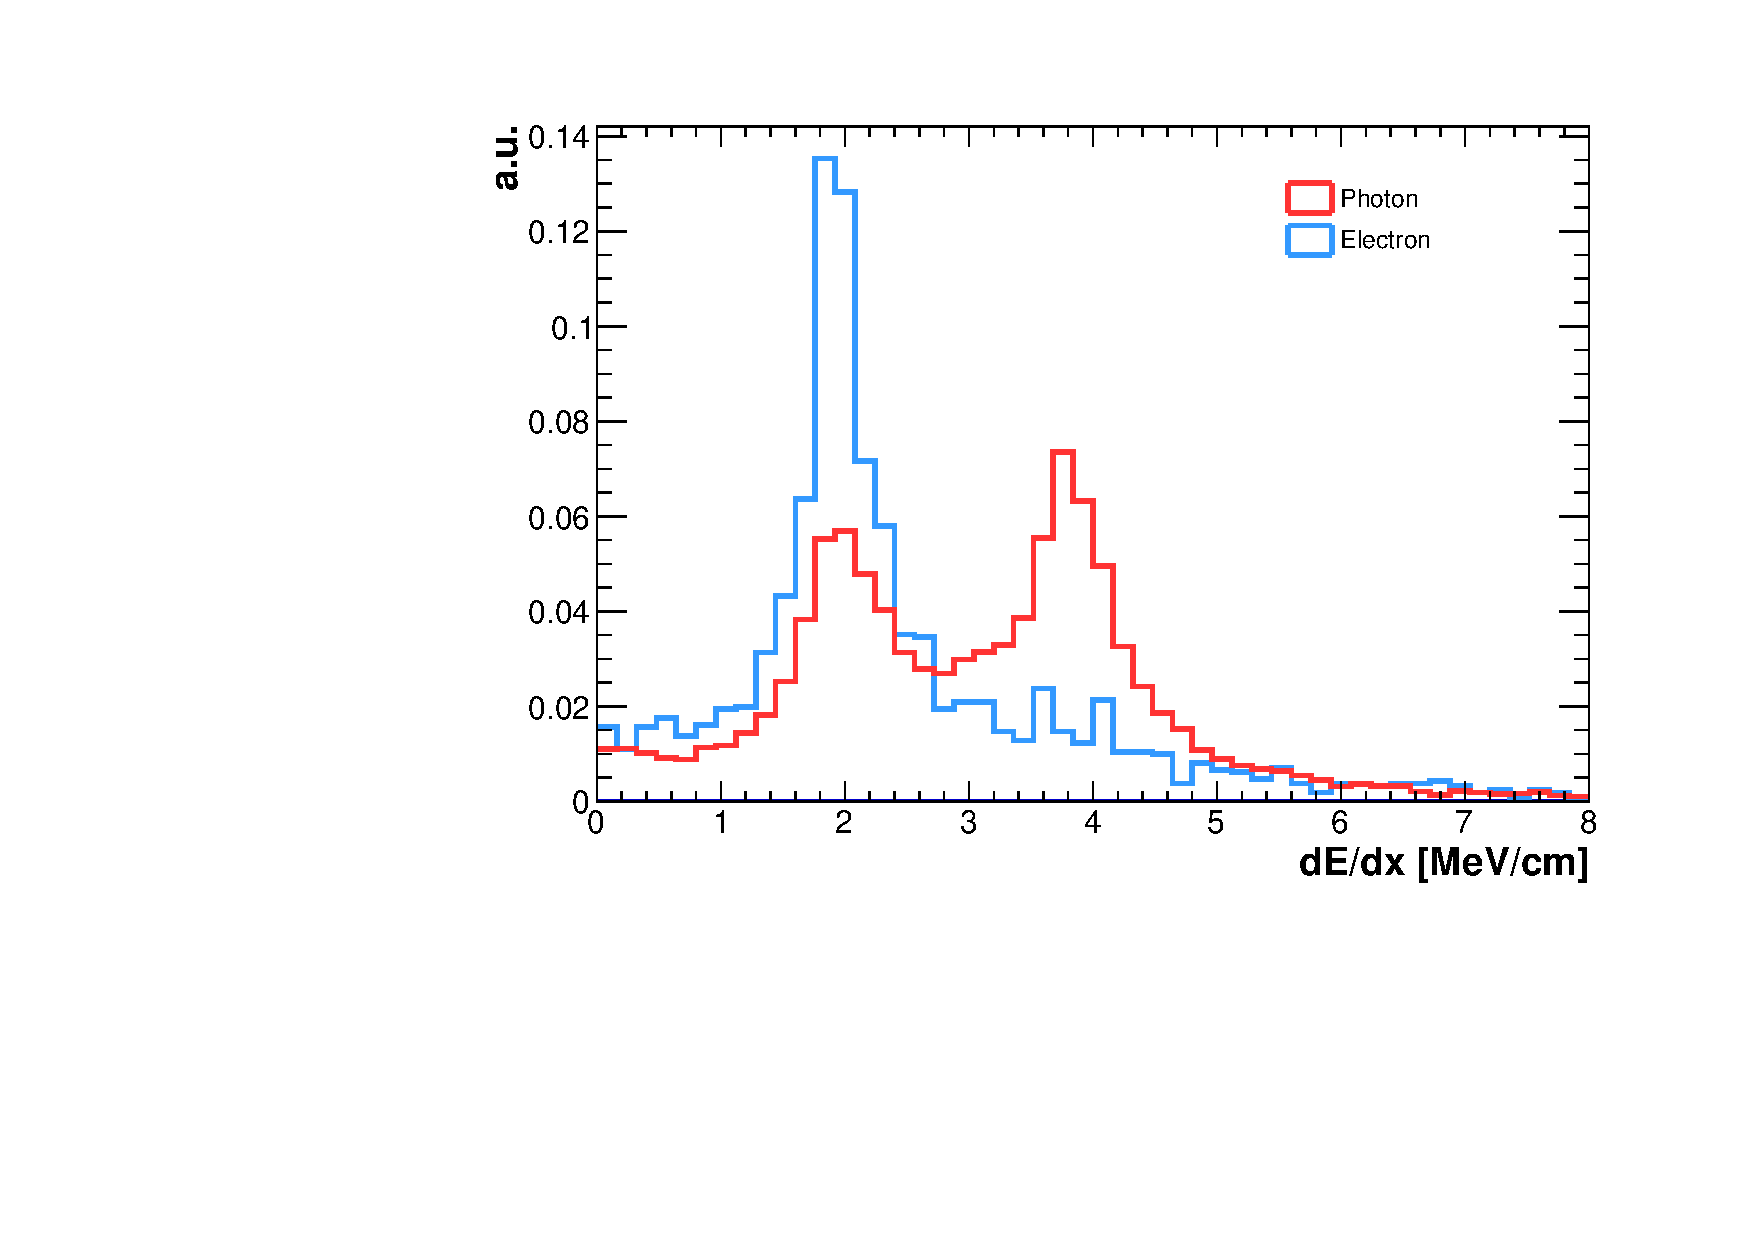
\includegraphics[width=\linewidth]{figures/dedx.pdf}
    \caption{$dE/dx$ median distribution} 
  \end{subfigure}
    \begin{subfigure}{0.45\textwidth}
    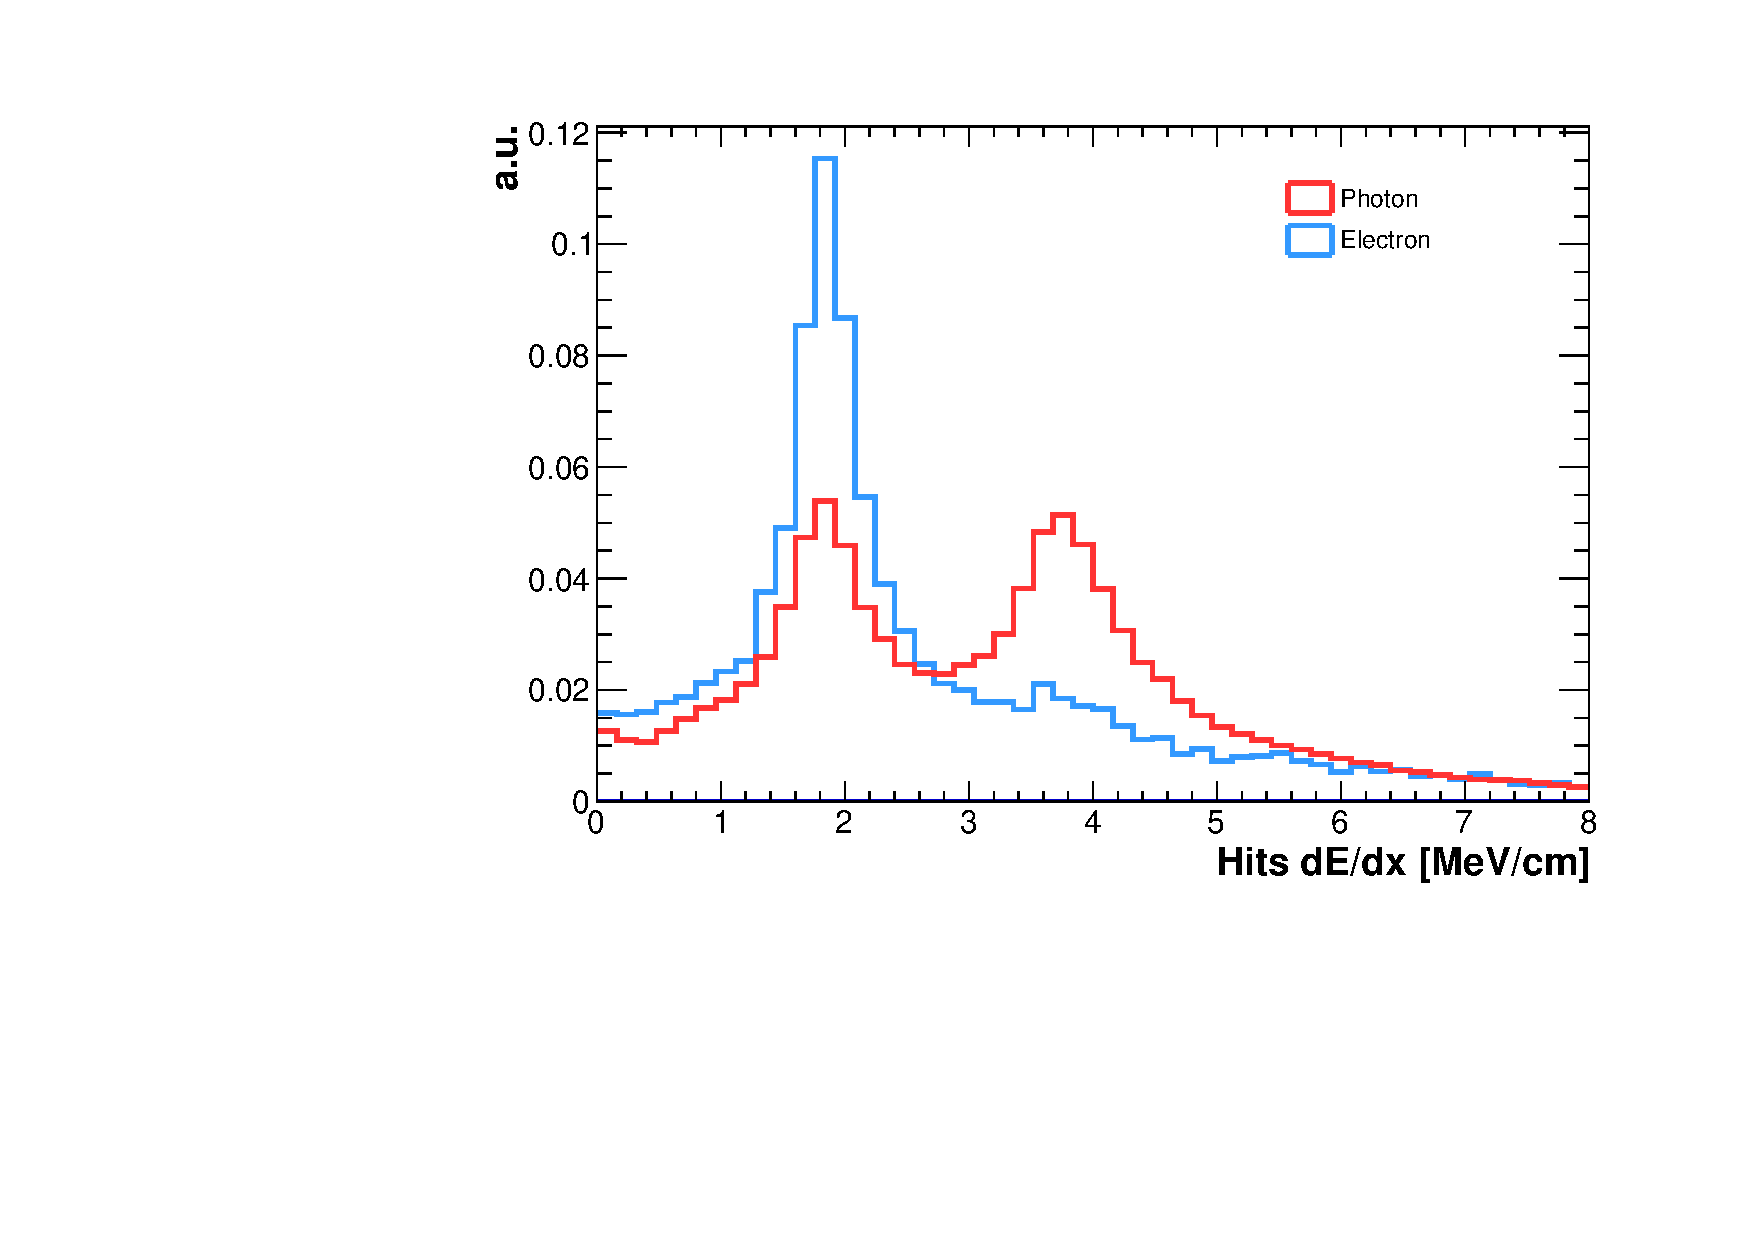
\includegraphics[width=\linewidth]{figures/hits_dedx.pdf}
    \caption{$dE/dx$ hit distribution} 
  \end{subfigure}
  \caption{$dE/dx$ median distribution (left) and the $dE/dx$ hit distribution (right) for electron and photon showers with at least 10 reconstructed hits.}\label{fig:dedx}
\end{figure}


The first peak is caused by low-energy photons and, to a lesser extent, Compton scattering. When a low energetic photon converts into a $e^+e^-$ pair, in the case of a very asymmetric decay, the electron (or the positron) can have a very low deposited energy. In this case, one of the two particle will travel for a much shorter distance than the 4~cm rectangle length, causing the median of the distribution to be 2~MeV/cm and not 4~MeV/cm \cite{caratelli}. Figure \ref{fig:dedx_energy} shows a bi-dimensional histogram of the $dE/dx$ vs. the reconstructed energy for simulated photon showers: as expected, the first peak is mainly caused by low-energy showers. In our sample, the cut applied on the most energetic shower is $1~\mathrm{MeV/cm} < dE/dx < 3.2~\mathrm{MeV/cm}$.


\begin{figure}[htbp]
\centering
  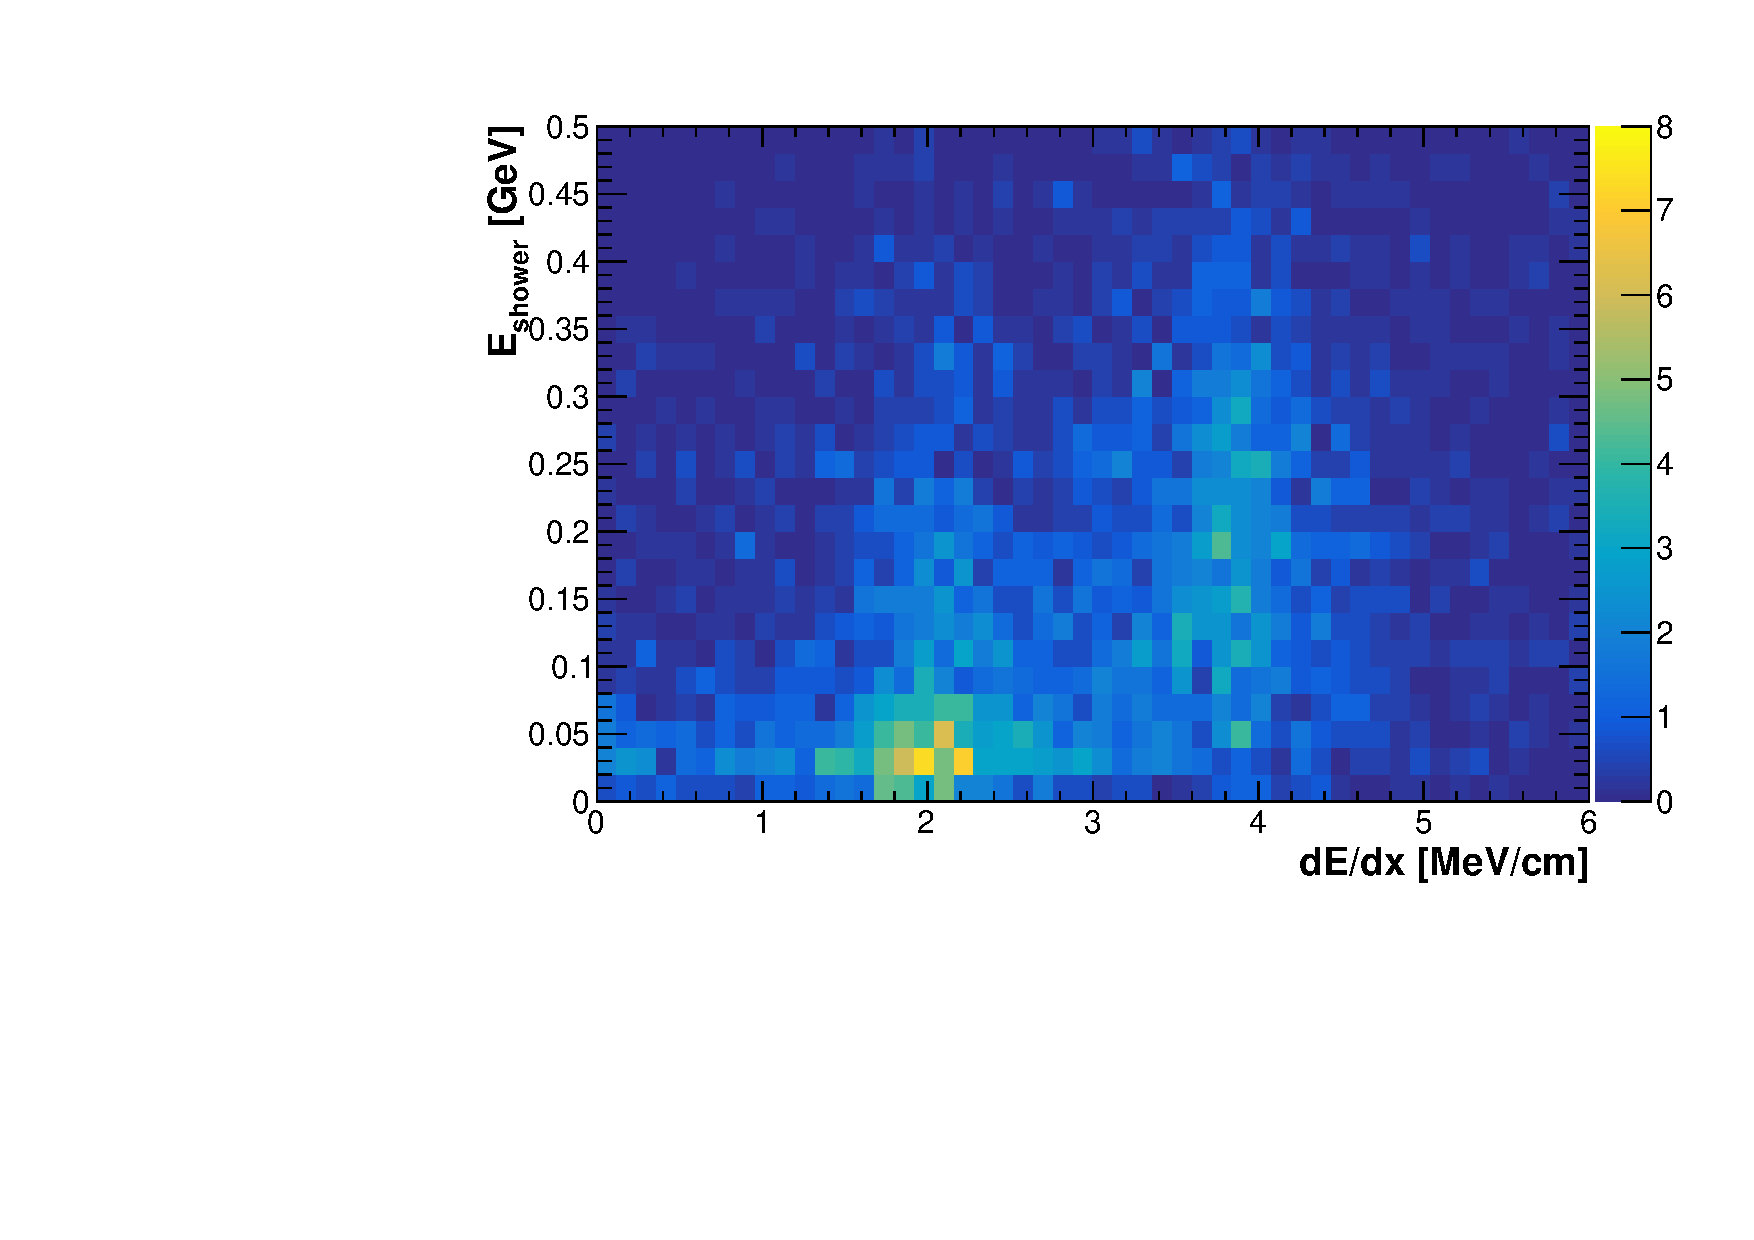
\includegraphics[width=0.7\linewidth]{figures/dedx_energy.pdf}
  \caption{$dE/dx$ vs. reconstructed shower energy $E_{\mathrm{shower}}$ for photon showers. The peak around 2 MeV/cm corresponds mainly to low-energy showers.}\label{fig:dedx_energy}
\end{figure}


\subsubsection{Shower energy}
The energy of each electromagnetic shower is measured with the procedure described in Section \ref{sec:showerenergy}. A large number of cosmic in-time events will have a low shower energy, mainly caused by Michel electrons. A significant portion of charged-current $\nu_{\mu}$ events will also have low-energy showers caused by stopping muons and spurious hits. A cut of 50 MeV on the reconstructed energy of the most energetic shower removes a large fraction of the cosmic in-time and CC $\nu_{\mu}$ backgrounds, without significantly reducing the $\nu_{e}$ CC0$\pi$-Np efficiency. 
% Figure \ref{fig:showerenergy} shows the reconstructed energy distribution of the most energetic shower in the low-energy region and the reconstructed energy spectrum after the shower energy cut.


\subsubsection{Proton track BDT}\label{sec:protbdt}
The aim of the analysis is to find $\nu_{e}$ CC$0\pi$-Np events. As such, it is necessary to identify events with non-proton tracks in the final state (e.g. pions and muons). A boosted decision tree (BDT) has been trained using the length of the track and its $dQ/dx$. The track $dQ/dx$ has been calculated by taking the median the $dQ/dx$ hit distribution. The training sample is a simulated dataset of BNB neutrino interactions with CORSIKA cosmic rays. The signal is defined as all the reconstructed tracks matched to simulated protons and the background as reconstructed tracks matched to simulated muons. Figure \ref{fig:bdt} shows the $dQ/dx$ as a function of the track length and the BDT score for proton tracks and muon tracks. At least a track in the event candidate is required to have a BDT score of at least -0.12, which corresponds to a signal efficiency of 98\% and a background rejection of 55\%. 

\begin{figure}[htbp]
\centering
  \begin{subfigure}{0.45\textwidth}
    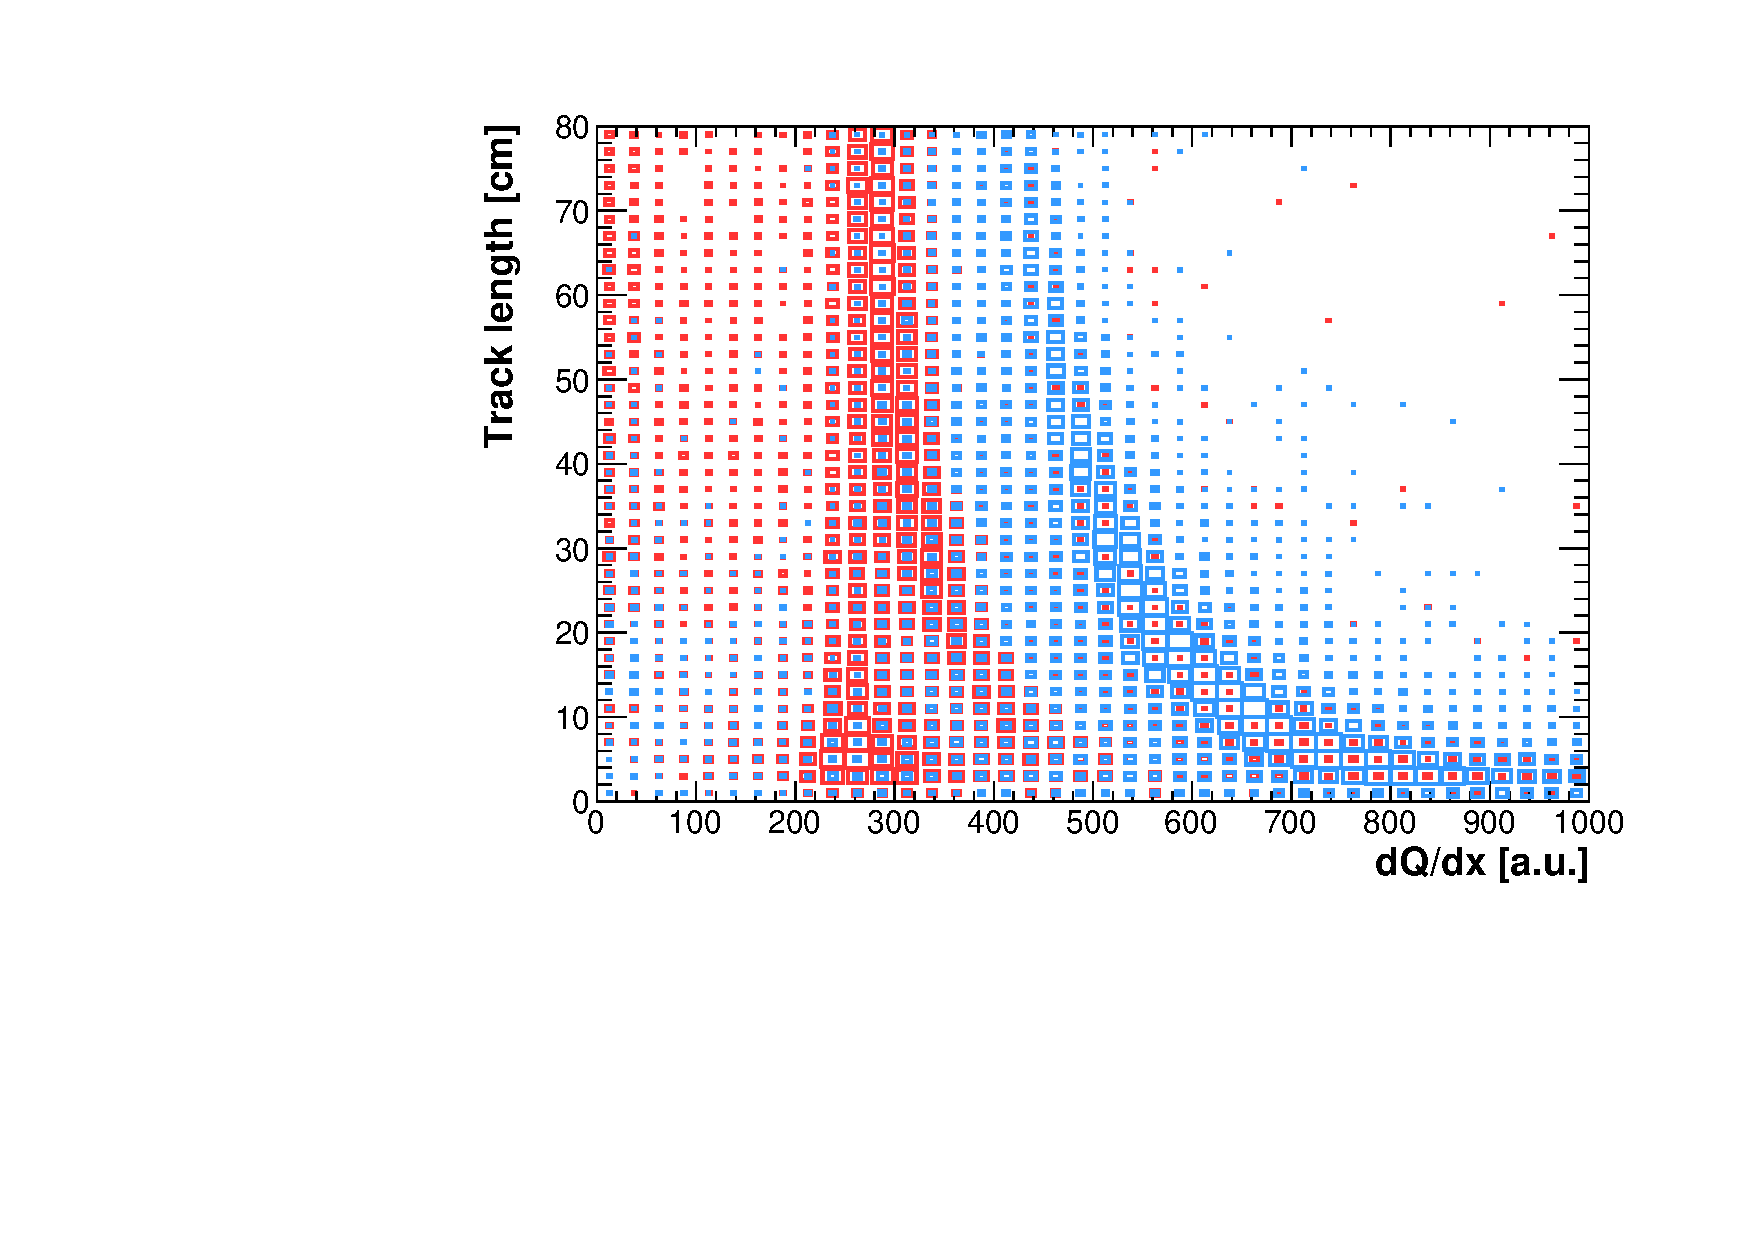
\includegraphics[width=\linewidth]{figures/dqdx.pdf}
    \caption{$dQ/dx$ as a function of track length.} 
  \end{subfigure}
    \begin{subfigure}{0.45\textwidth}
    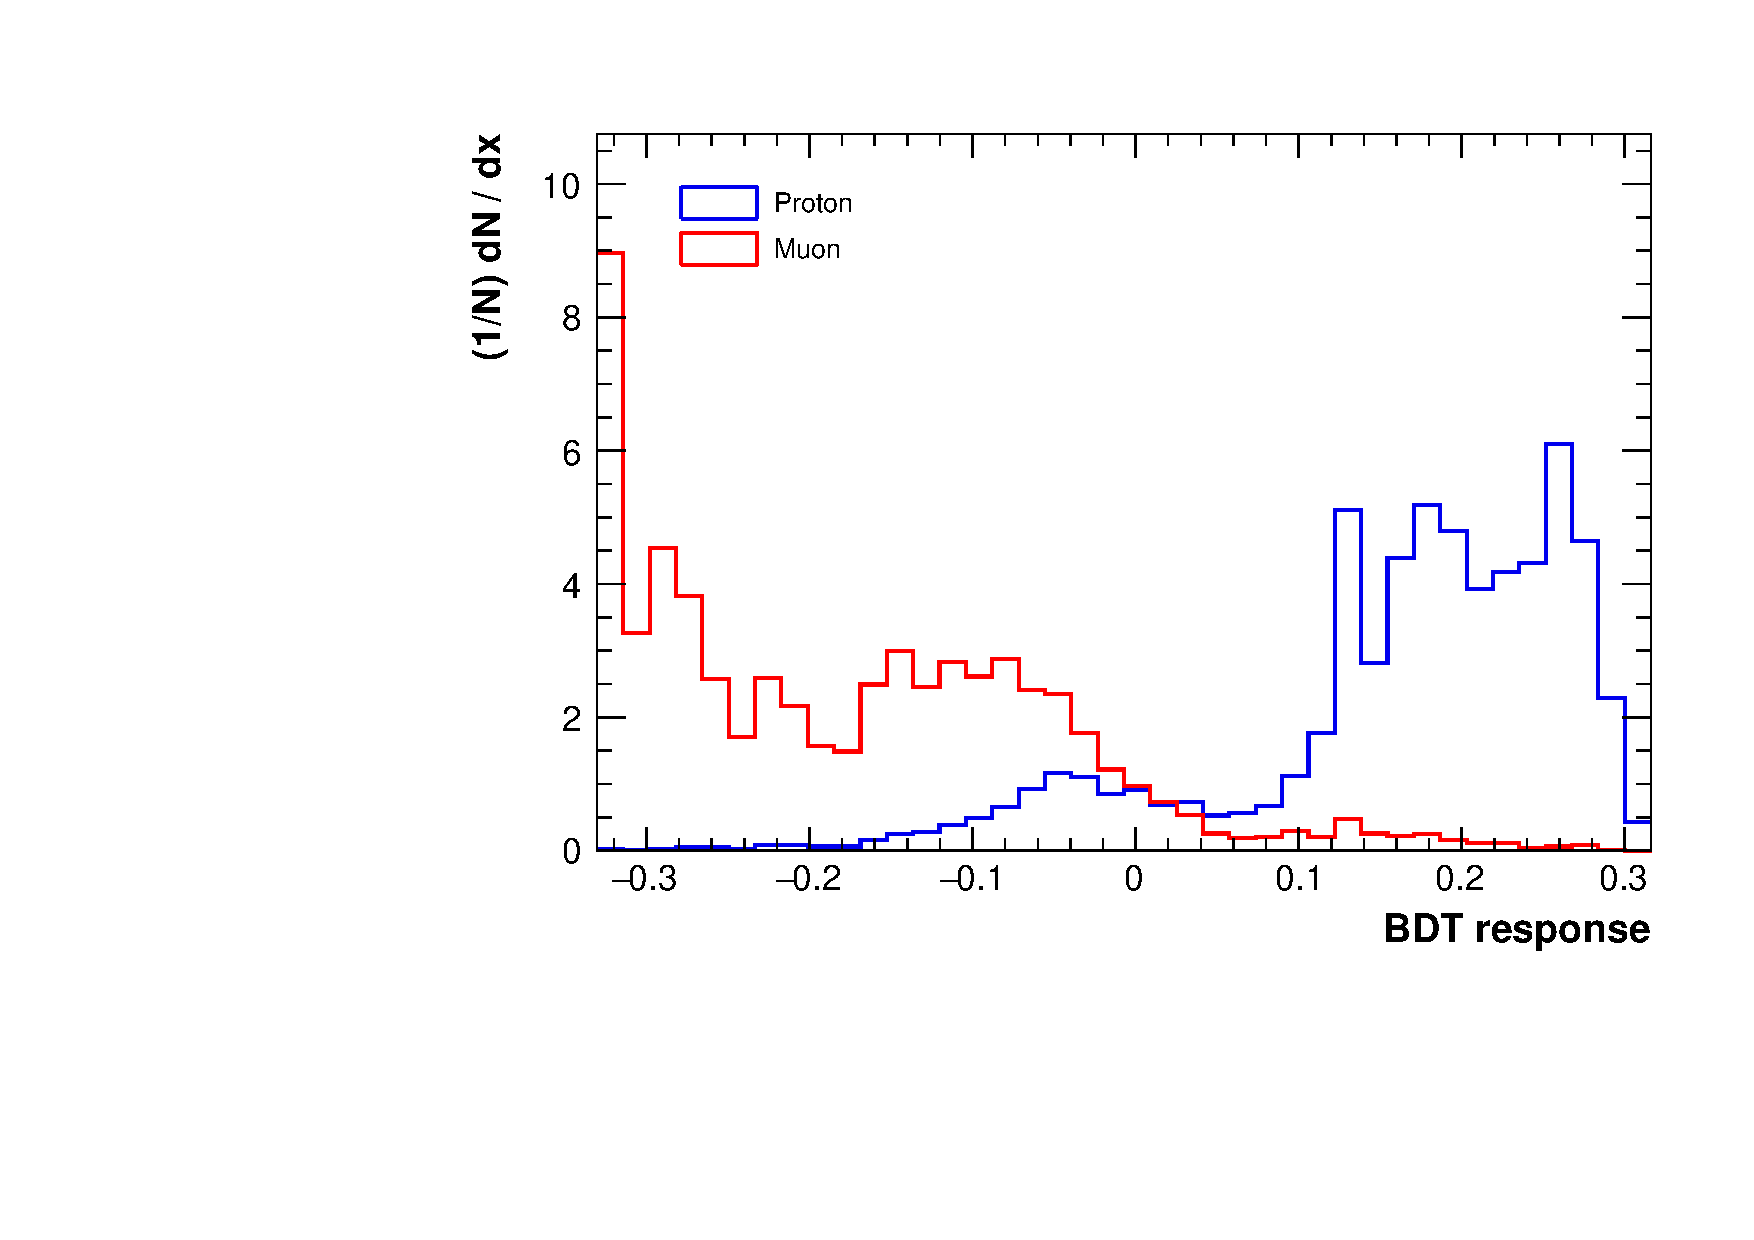
\includegraphics[width=\linewidth]{figures/bdt.pdf}
    \caption{BDT score.} 
  \end{subfigure}
  \caption{Proton-like tracks are chosen from the score of a boosted decision tree, trained using the track length and the $dQ/dx$ for reconstructed protons (blue) and muons (red).}\label{fig:bdt}
\end{figure}

\subsubsection{Track distance}
A well reconstructed event with a proton in the final state will have a reconstructed track close to the reconstructed neutrino vertex. However, the requirement on the distance between the reconstructed track and the reconstructed neutrino vertex can not be too strict, due to the limited neutrino vertex spatial resolution. Figure \ref{fig:dist} shows the histogram of the distance between the true neutrino vertex (corrected by the space-charge effect \cite{sce}) and the reconstructed neutrino vertex for simulated $\nu_{e}$ CC0$\pi$-Np events. The most proton-like track, chosen using the score assigned by the procedure described in Section \ref{sec:protbdt}, is required to be within 3~cm the reconstructed neutrino vertex ($d_t < 3$~cm).

\begin{figure}[htbp]
\centering
  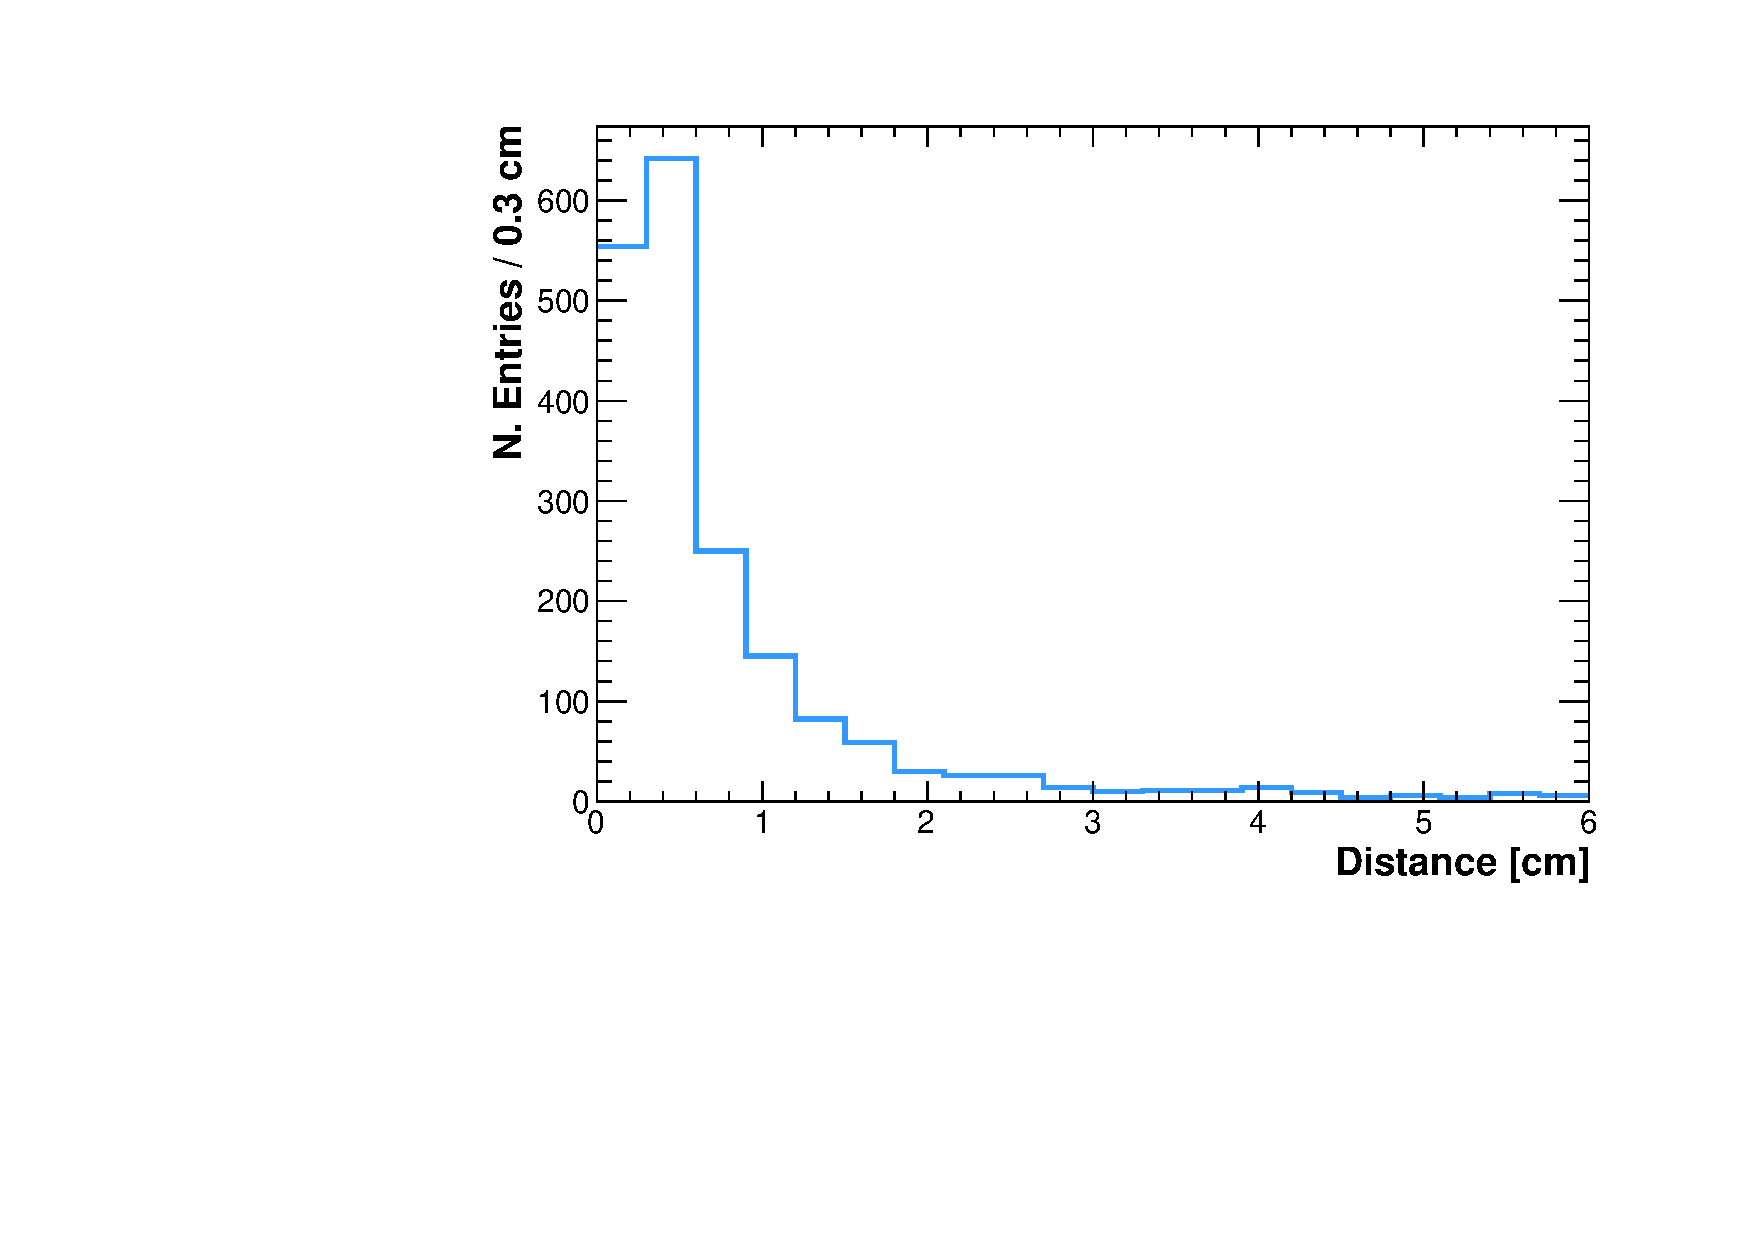
\includegraphics[width=0.7\linewidth]{figures/dist.pdf}
  \caption{Distance between the reconstructed neutrino vertex and the true neutrino vertex, corrected by the space-charge effect, for $\nu_{e}$ CC0$\pi$-Np simulated events.}\label{fig:dist}
\end{figure}

\subsubsection{Shower distance}
Liquid argon TPC such as MicroBooNE can distinguish between photons and electrons in two ways: (1) measuring the $dE/dx$ of the electromagnetic shower (as described in Section \ref{sec:dedx}), and (2) measuring the gap between the interaction vertex and the start of the electromagnetic shower. In fact, photons produced in the final state of the neutrino interaction can travel several centimeters without interacting. In order to suppress events with a photon in the final state, the leading shower starting point is required to be within 10 cm  the reconstructed neutrino vertex ($d_{s} < 10$~cm).

\subsubsection{Track-shower angle}
Low-energy electrons often start producing an appreciable shower in the detector after several centimeters. As such, the reconstruction framework identifies the first part of the shower as a track-like object and the last part of the shower as a shower-like object. 
Furthermore, high-energy cosmic rays can produce a shower in the detector, which will be mostly aligned to the track. In order to remove these mis-reconstructed events and reduce this kind of cosmogenic background we require $\mathrm{cos}\theta > -0.9$, where $\theta$ is the angle between the most energetic shower and the most proton-like track, as identified by the procedure described in Section \ref{sec:protbdt}.
Figure \ref{fig:angle} shows the event displays of a cosmic ray showering in the last part and of an electron shower being reconstructed as a track-like object plus a shower-like object.

\begin{figure}[htbp]
\centering
  \begin{subfigure}{0.45\textwidth}
    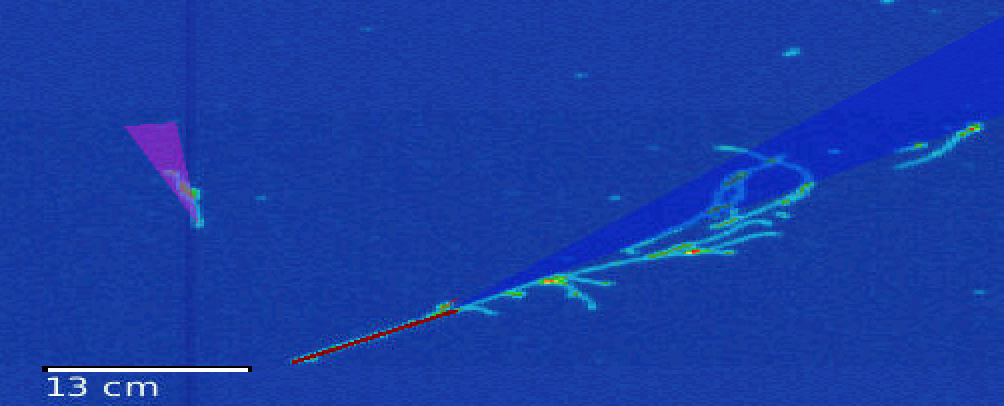
\includegraphics[width=\linewidth]{figures/angle1.png}
    \caption{Cosmic-ray shower} 
  \end{subfigure}
    \begin{subfigure}{0.45\textwidth}
    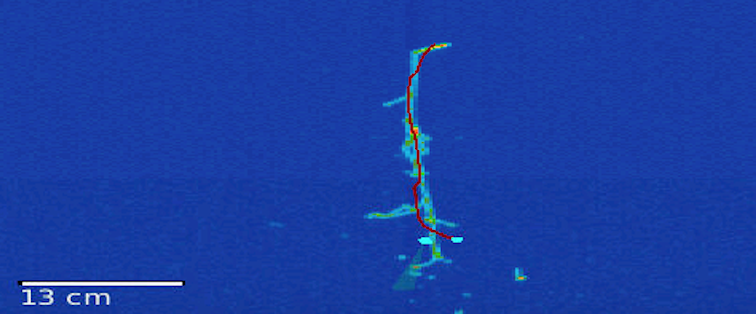
\includegraphics[width=\linewidth]{figures/angle2.png}
    \caption{Electron shower} 
  \end{subfigure}
  \caption{Monte Carlo event displays of a cosmic ray showering in the detector (left) and of an electron shower (right). Both objects were reconstructed in the first part as a track-like object and in the last part as a shower-like object}\label{fig:angle}
\end{figure}


\subsubsection{Shower opening angle}
Reconstructed showers corresponding to low-energy electrons will have in general a small opening angle $\theta$. Requiring the most energetic shower to be smaller than $20^{\circ}$ and larger than $1^{\circ}$ allows to reduce the background component without significantly impacting the signal efficiency. In this way we are able to reject $\nu_{\mu}$ CCDIS events and high-energetic cosmic-ray events, which will have larger opening angles. The requirement on the minimum value of the opening angle allows also to reject events with tracks mis-reconstructed as shower-like objects.

\subsubsection{Track length}
Our signal sample will contain only protons in the final state. Protons in liquid argon have a higher stopping power than muons, which will correspond on average to shorter tracks. Each reconstructed track in the selected sample is required to be shorter than 80 cm. This cut helps rejecting mainly CC $\nu_{\mu}$ events with high-energy muons in the final state.
Thus, an increased size of the unblinded data sample could allow us to apply more efficient cuts.

% \subsection{Optical selection}


% \subsection{Topology requirement}

% Energy reconstruction section should have the following sections:
% Shower Reconstruction (Inlucding resoltuion, validation with pi0)
% track reconstruction (Length based methodology, resolution)
%	- Hadronic energy reconstruction (All tracks in a selected neutrino interaction)
% Neutrino Energy Reconstruction

\section{Energy reconstruction}\label{sec:energyreco}
\subsection{Scope of the reconstruction}
In this analysis we restrict ourselves to the measurement of the deposited energy in the TPC of the visible particles in the final state of the neutrino interaction. Our signal will have in its final state, by definition, one electron and at least one proton, with no other visible particles. The energy of the electron will be measured by converting the hit charge of all the shower-like objects into deposited energy, as described in Section \ref{sec:showerenergy}. The energy of the protons, instead, can be measured by converting the track length of the reconstructed tracks into deposited energy, using the tabulated stopping power of protons in the liquid argon, with the procedure described in \ref{sec:protonenergy}.


\subsection{Electron energy reconstruction and calibration}\label{sec:showerenergy}
The reconstructed energy $E_{reco}^{e}$ of a shower-like object is measured converting the charge of the associated hits into deposited energy in the TPC. It is calculated by multiplying the reconstructed charge ($e^{-}_{reco}$) from hits associated with the reconstructed shower by the calibration factor measured in \cite{michel}:
\begin{equation}
\frac{E_{reco}^{e} \mathrm{(MeV)}}{e^-} = 1.01\frac{e^-}{e^{-}_{reco}} \times \frac{23.6~\mathrm{eV}}{e^-} \times 10^{-6} \frac{\mathrm{eV}}{\mathrm{MeV}} \times \frac{1}{R},\label{eq:calib}
\end{equation}
where:
\begin{itemize}

\item the correction factor $1.01\frac{e^-}{e^{-}_{reco}}$ is obtained measuring the true number of collected electrons $e^{-}$ on the wires using a sample of stopping muons, fitting the $dE/dx$ vs. residual range to values for argon as tabulated by the PDG \cite{pdg},
\item $\frac{23.6~\mathrm{eV}}{e^-}$ is the work function for ionizing an argon atom \cite{workfunction},
\item $R = 0.62$ is the recombination factor obtained with the Modified Box Model \cite{boxmodel}.
\end{itemize}
Figure \ref{fig:ecalib} shows the calibration slope necessary to convert the electron reconstructed energy $E_{reco}^{e}$ into true electron energy $E_{true}^{e}$. It has been obtained using only the hits reconstructed in the collection plane. 
The reconstructed energy is obtained summing the hits energy from each reconstructed shower matched to the true electron. The true electron and the reconstructed showers are required to be fully contained within the fiducial volume. Since the reconstructed energy distributions in each true energy bin is asymmetrical, the data points are obtained fitting a Gaussian around the peak of the distribution.
A linear fit of the data points gives:
\begin{equation}
E_{reco}^{e} = 0.78~E^{e} - 0.02~\mathrm{GeV}.
\end{equation}

\begin{figure}[htbp]
\centering
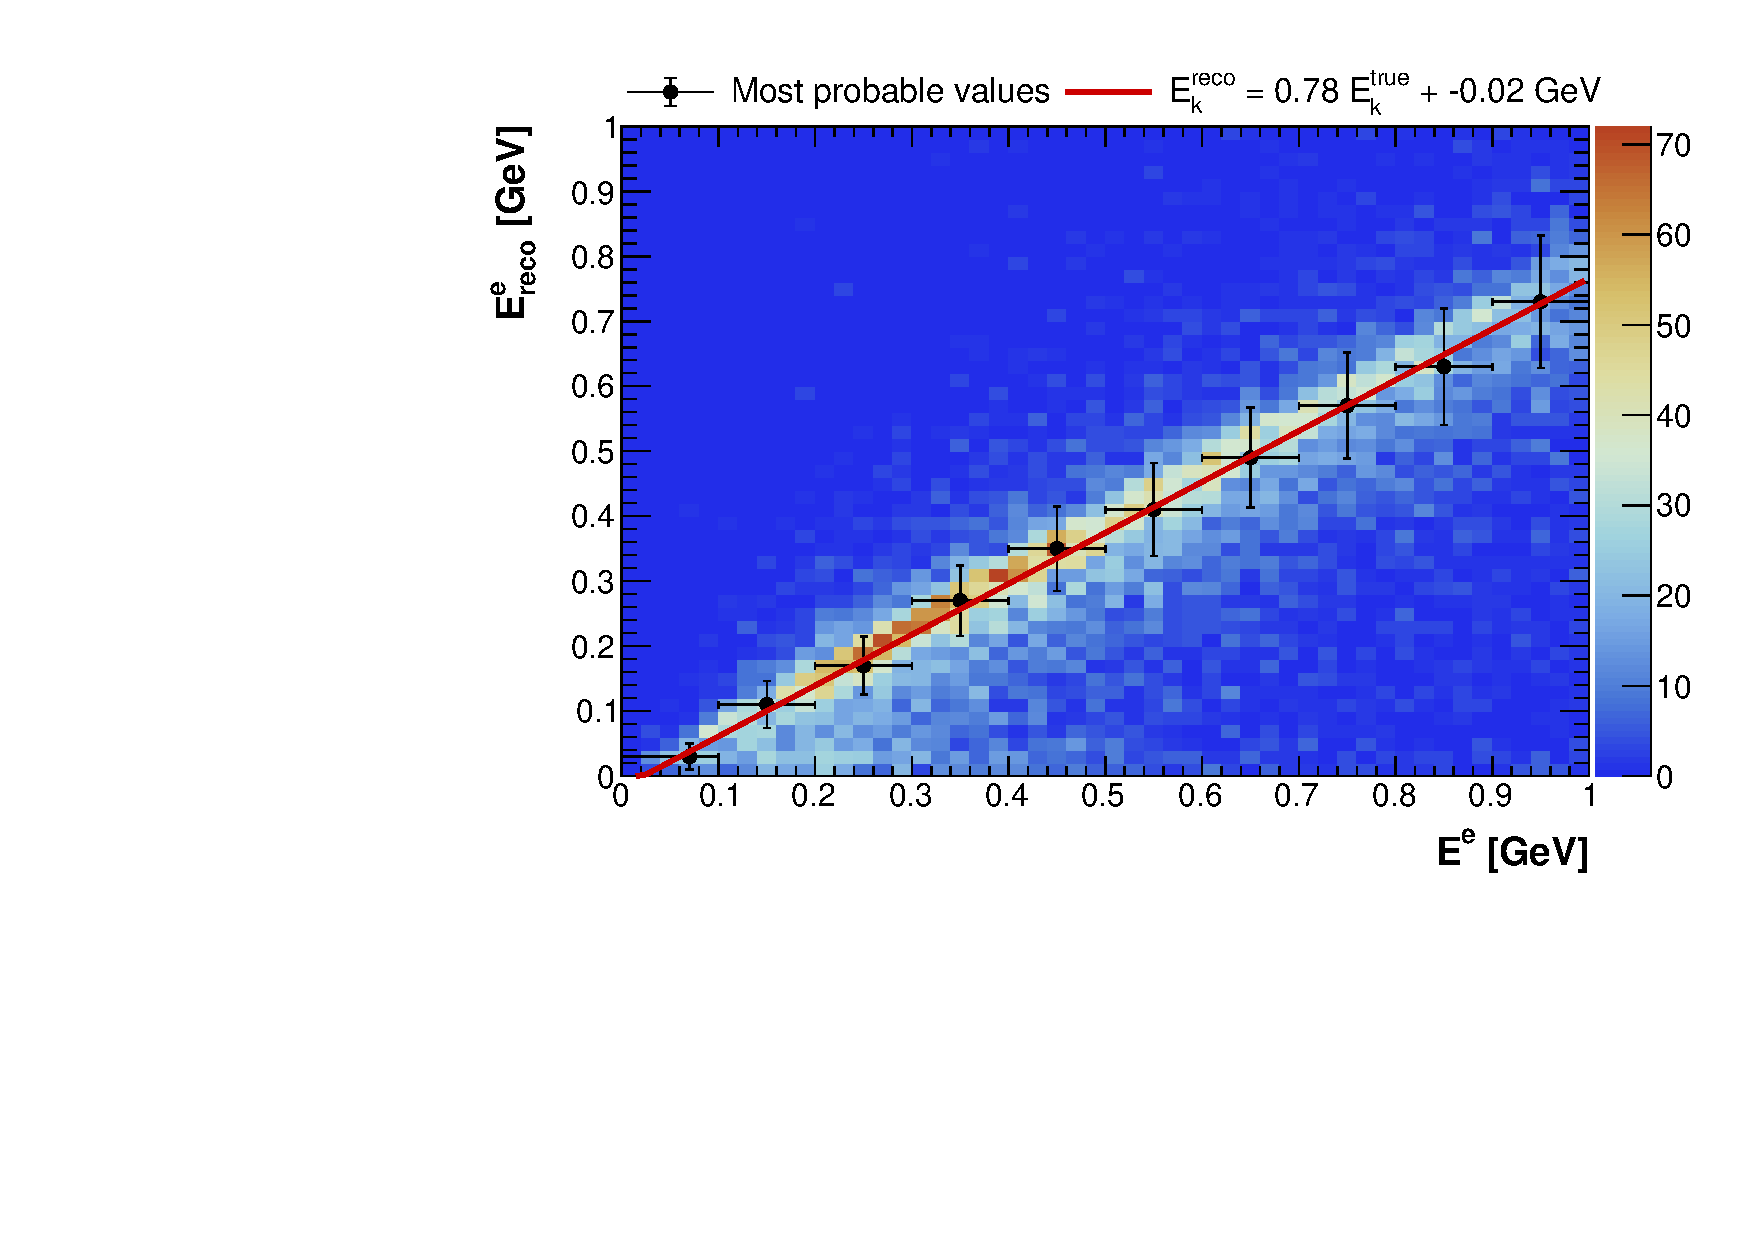
\includegraphics[width=0.65\columnwidth]{figures/ecalib.pdf}
\caption{Bi-dimensional histogram of true electron energy $E^{e}$ vs. reconstructed electron energy $E_{reco}^{e}$. Black points are obtained measuring the most probable value of the $E_{reco}^{e}$ distribution for each $E^{e}$ bin.}
\label{fig:ecalib}
\end{figure}



\subsubsection{\texorpdfstring{$\pi^0$}{pi0} mass peak}

CC$\pi^0$ events have been studied in order to validate the energy scale and reconstruction in the low-energy region in data as well as in the Monte Carlo. There is no aim for an analysis in the CC$\pi^0$ channel. Instead the purpose is to exploit a pure sample of $\pi^0$ decays, which can be used as standard candle to validate the energy reconstruction.
The samples which have been used are:
\begin{itemize}
  \item Data: hand scanned CC$\pi^0$ sample, which has been already used in \cite{caratelli}
  \item Monte Carlo: BNB intrinsic $\nu_{\mu}$ with cosmic rays. generator level requirements:
\end{itemize}
The optical selection, described in section \ref{sec:optical_pre_cuts}, and the topological pre-selection, described in section \ref{sec:topological_pre_selection}, are applied to both samples.\\
An additional set of generator level requirements is applied to the Monte Carlo sample, in order to identify CC$\pi^0$ using truth information:
\begin{itemize}
    \item The selected neutrino interaction must be matched to the true neutrino interaction
    \item The interaction must be a charged current interaction
    \item Exactly one $\pi^0$ must be present in the final state
\end{itemize}
Subsequently events are required to have at least two reconstructed showers, both with hits on the collection plane. The second requirement is meant to remove events with null shower energy, as the energy is computed from the collection plane only. The energy of the showers is calibrated as shown previously in section \ref{sec:showerenergy}, deriving correction factors from electrons-matched-showers using the simulation, as shown in Figure \ref{fig:ecalib}.
The $\pi^0$ candidate is computed starting from the two most energetic showers. The distribution of the number of reconstructed showers in each event is shown in the left plot in Figure \ref{fig:mc_mass_e2} for data and MC.

As there are many events with more than two showers, about two thirds in data and one half in Monte Carlo, a simple re-clustering of the energy is performed. It is meant to recover the energy from broken showers. The two most energetic showers are considered. Then, the energy of any additional shower is summed to the closest in angle among the two most energetic showers. The direction of the two most energetic showers is not modified in this process. The mass is computed from the two most energetic showers, with the energy corrected after the re-clustering, as:
\[ M = \sqrt{E_1 E_2 (1 - \cos\theta)} \]
where $E_1$ and $E_2$ are the energies of the most and the second most energetic showers, respectively. $\theta$ is the 3-D angle between the directions of the two showers.

\begin{figure}[!htbp]
\centering
\begin{minipage}{0.49\columnwidth}
  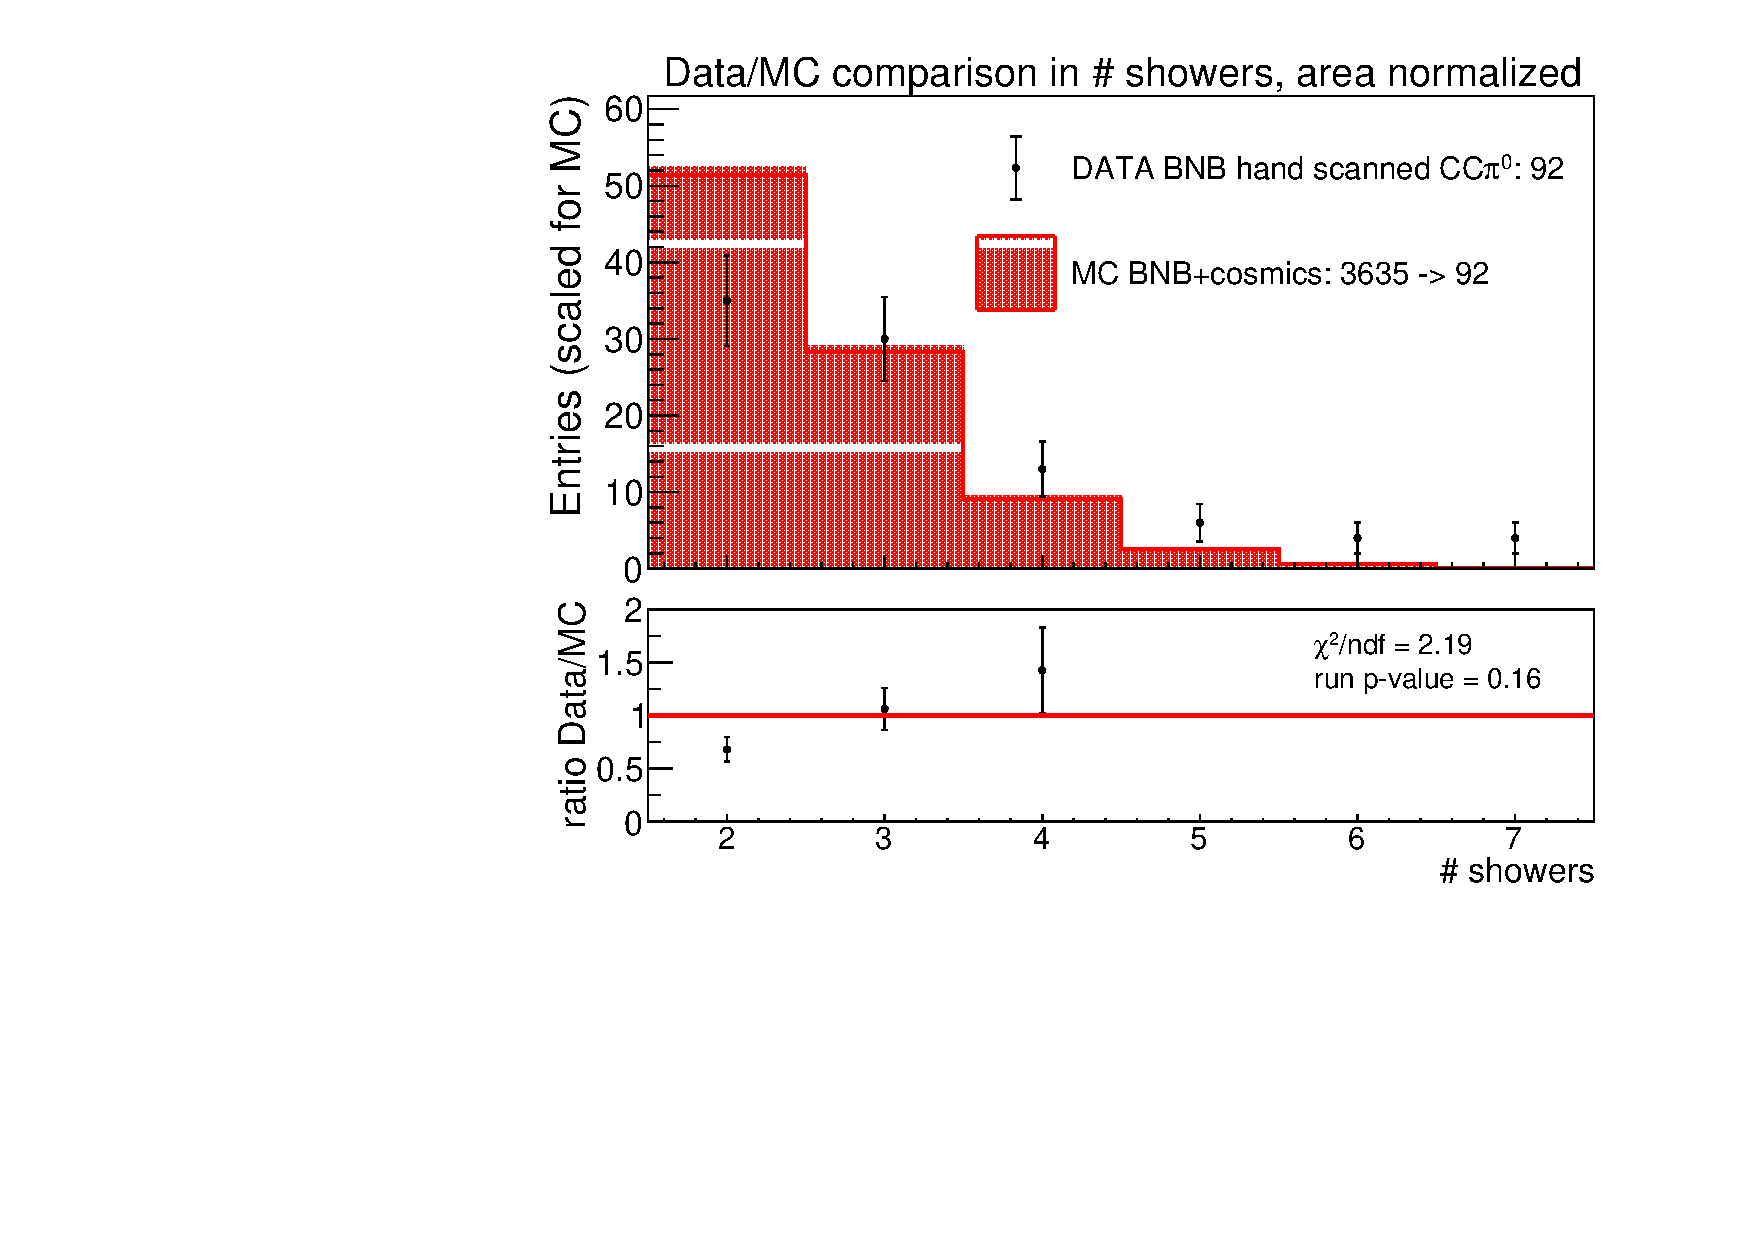
\includegraphics[width=0.99\columnwidth]{figures/n_showers_data_MC_comparison_mod.pdf}
\end{minipage}
\begin{minipage}{0.49\columnwidth} 
  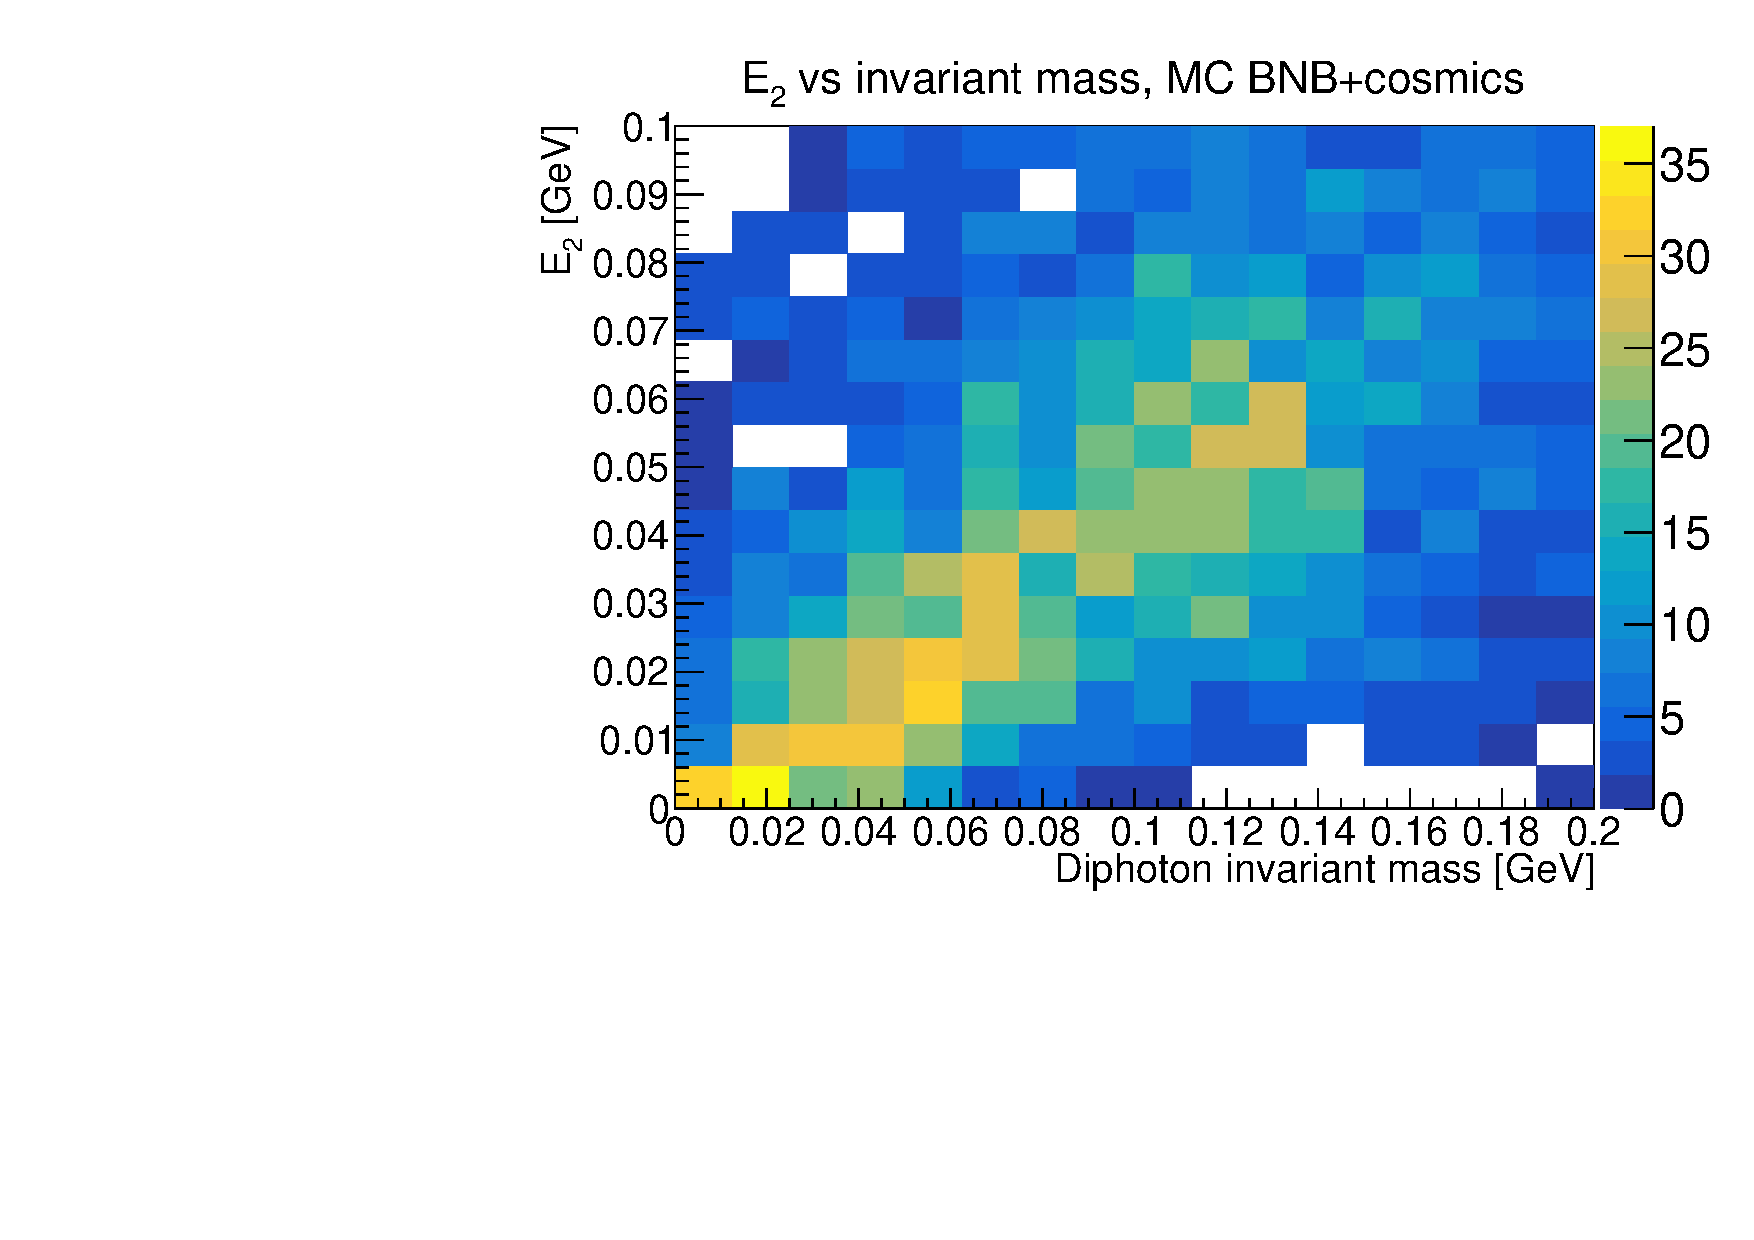
\includegraphics[width=0.99\columnwidth]{figures/MC_mass_E2.pdf}
\end{minipage}
\caption{Left: Distribution of the number of showers for each event, for data (black dots) and Monte Carlo (red boxes). Right: Bi-dimensional distribution of $E_2$ (y-axis) versus the invariant mass (x-axis) in Monte Carlo events.}
\label{fig:mc_mass_e2}
\end{figure}

In some cases a significant amount of energy is missing. For instance, one of the two main showers is missed, and a smaller shower, resulting from noise or from mis-reconstruction of other objects, is taken as one of the decay products of the $\pi^0$. The right plot in Figure \ref{fig:mc_mass_e2} shows the bi-dimensional distribution of the invariant mass (x-axis) versus $E_2$ (x-axis) for Monte Carlo events. As it is possible to see, a significant amount of events has small $E_2$ and small mass. Thus, to take into account this effect and remove events with one shower badly or mis-reconstructed, the second most energetic shower is required to have reconstructed energy larger than 30~MeV.

The final peak after the selection is shown in Figure \ref{fig:pi0_mass_peak}. The two histograms, for data and Monte Carlo, are fitted through a binned maximum likelihood (ML) fit with a crystal ball function, which consists of a Gaussian core, $C^1$-matched with a power-law right tail. The fit result, for what concerns the core is:
\[ \text{Data:} \quad \mu = 133 \pm 7~\text{MeV}, \quad \sigma = 47 \pm 5~\text{MeV} \]
\[ \text{Monte Carlo:} \quad \mu = 119 \pm 2~\text{MeV}, \quad \sigma = 51 \pm 2~\text{MeV} \]

The two results are significantly close to the nominal mass of 135~MeV, and shows a relatively good agreement between data and Monte Carlo. However, the discrepancy is significant and requires more investigation, in order to be understood completely.

\begin{figure}[htbp]
\centering
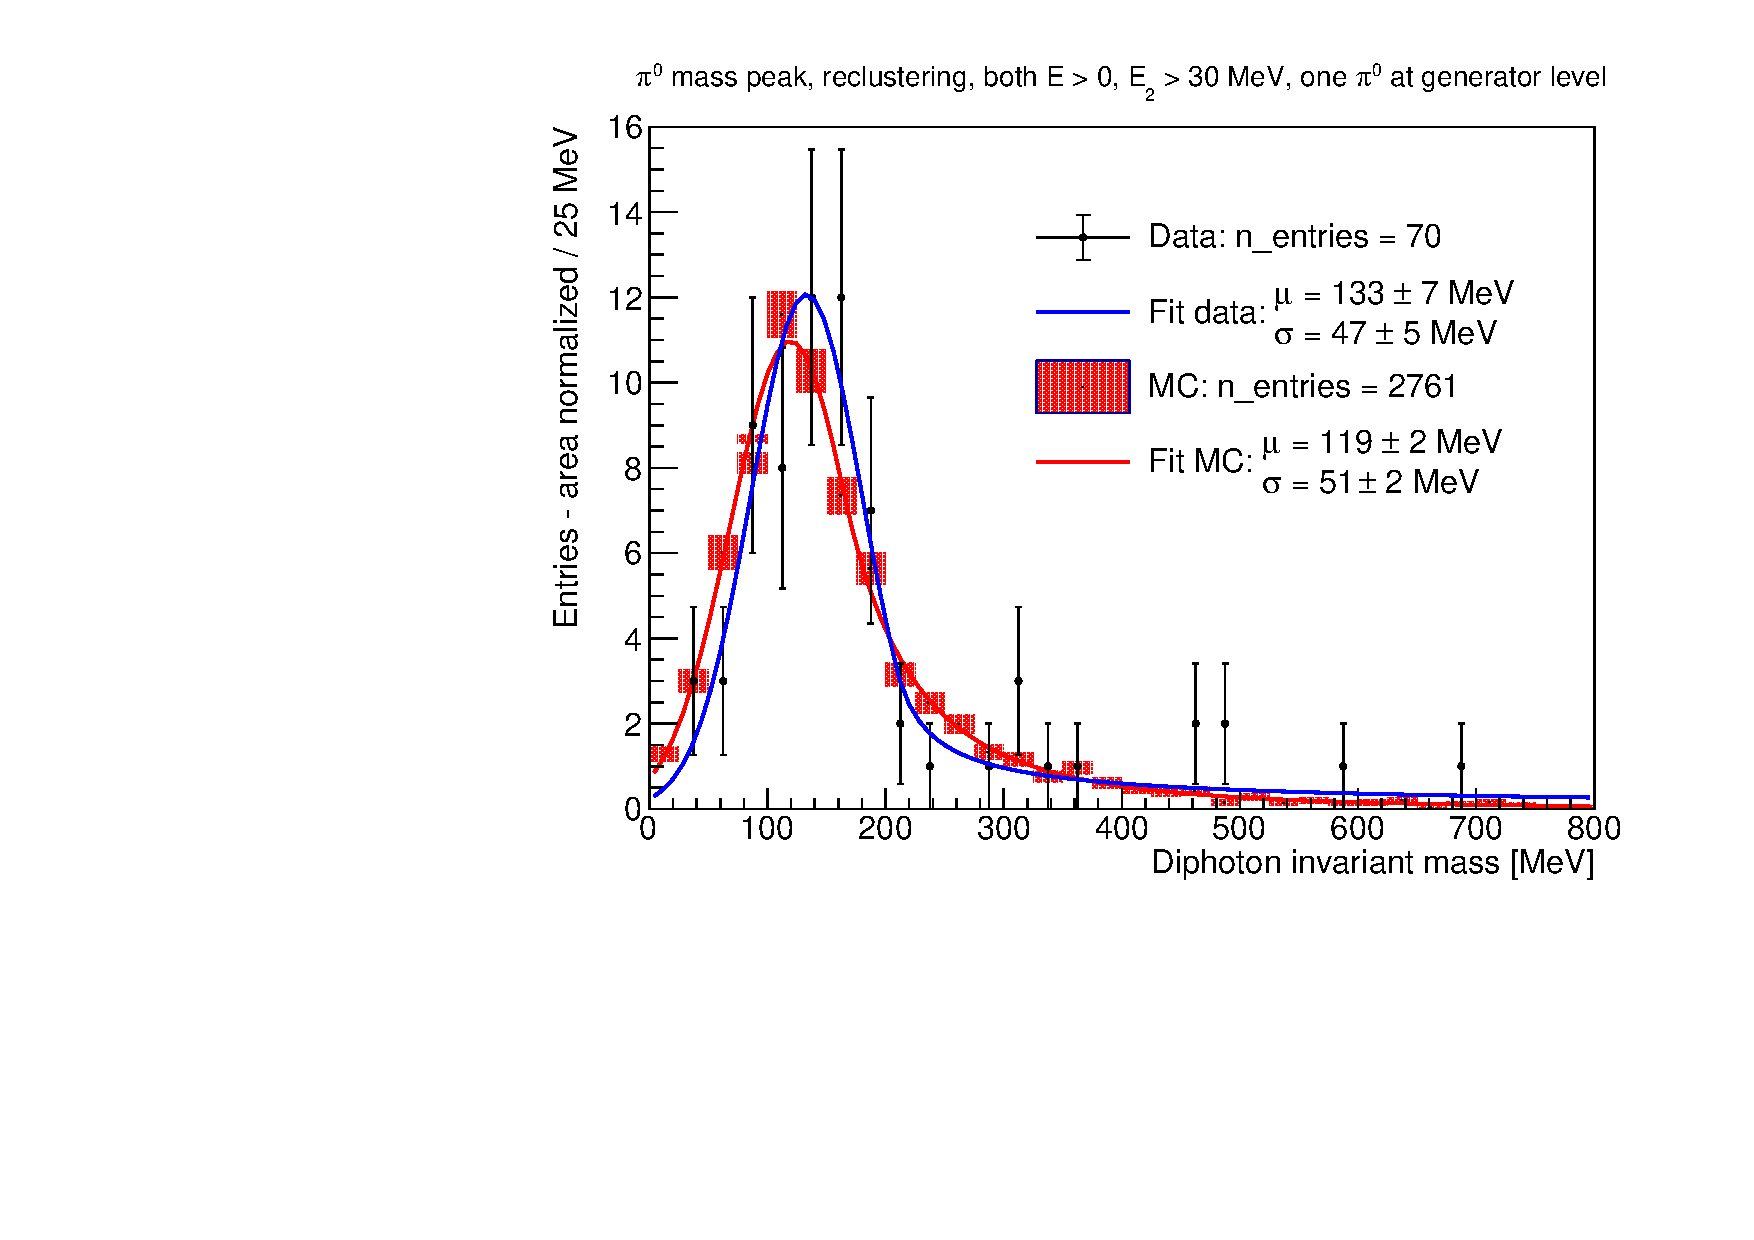
\includegraphics[width=0.65\textwidth]{figures/pi0_mass_peak_final.pdf}
\caption{Diphoton invariant mass distribution for data and Monte Carlo. The two lines show the crystal ball functions as obtained from the ML fit to the two histrograms.} 
\label{fig:pi0_mass_peak}
\end{figure}

% \subsection{Hadronic Energy Reconstruction}
\subsection{Single proton energy reconstruction and calibration}\label{sec:protonenergy}
Proton energy reconstruction is obtained converting the reconstructed track length $L$ into deposited energy using the proton stopping power in liquid argon, as tabulated in \cite{pstar}. Liquid argon density $\rho_{\mathrm{LAr}}$ is assumed to be constant at 1.379~g/ml. Figure \ref{fig:proton} shows the proton kinetic energy as a function of the range of the proton in liquid argon (measured as $L \times \rho_{\mathrm{LAr}}$) .

\begin{figure}[htbp]
\centering
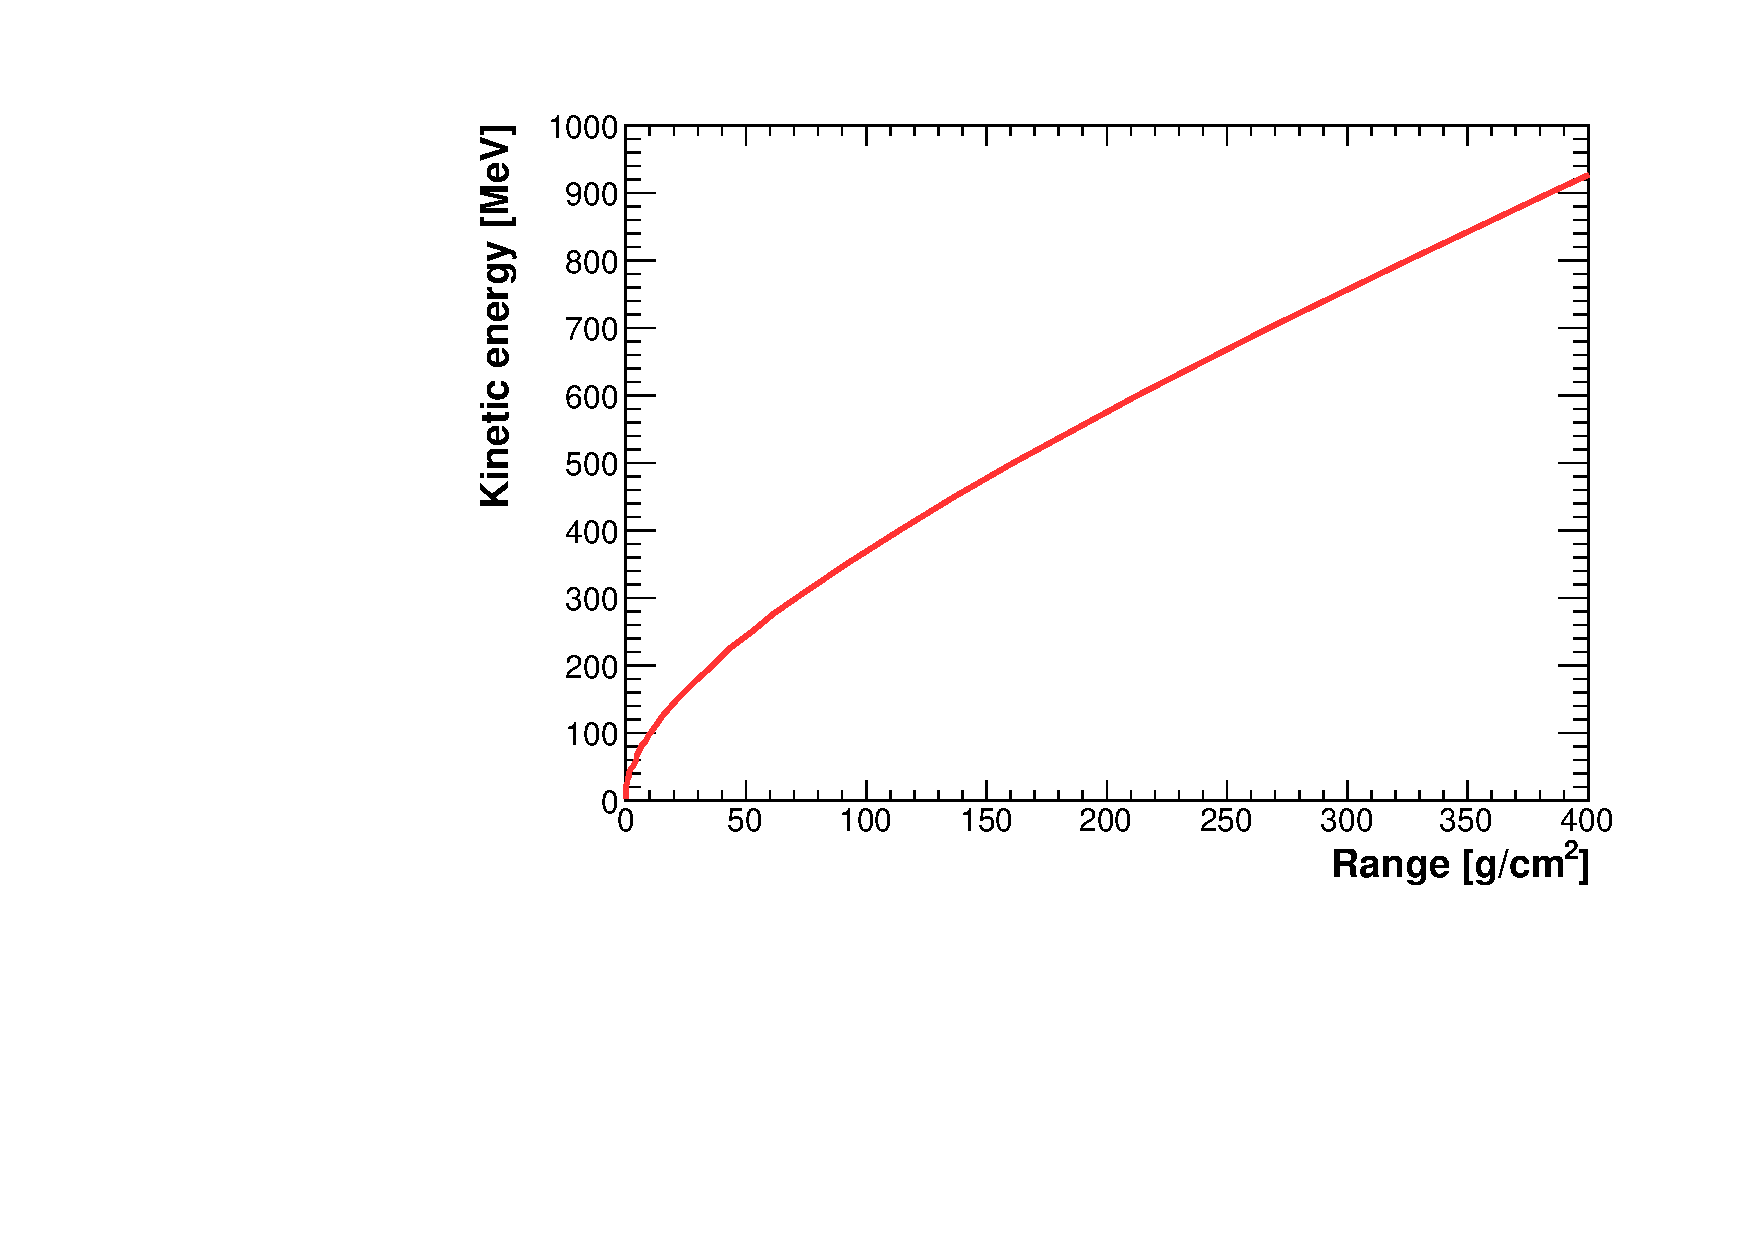
\includegraphics[width=0.65\textwidth]{figures/proton.pdf}
\caption{Proton kinetic energy as a function of the range of the proton in liquid argon. Values are taken from \cite{pstar}.} 
\label{fig:proton}
\end{figure}

The calibration constant has been obtained comparing the reconstructed energy of the proton with the true kinetic energy of the proton, in a CC $\nu_{e}$ sample with only one proton in the final state. The true proton and the reconstructed tracks are required to be fully contained within the fiducial volume. Since protons are not MIPs, in the case of two or more tracks (\emph{split tracks}) associated to the same proton, the reconstructed length of the tracks has been summed before calculating the corresponding kinetic energy.
Figure \ref{fig:pcalib} shows the calibration slope necessary to convert the proton reconstructed energy $E_{reco}^{p}$ into true proton kinetic energy $E_{true}^{p}$. For each bin of the true proton energy, the most probable value of the corresponding proton reconstructed energy has been obtained with a Gaussian fit around the peak of the distribution. A linear fit of the data points gives:
\begin{equation}
E_{reco}^{p} = 0.99~E^{p}.
\end{equation}

\begin{figure}[!htbp]
\centering
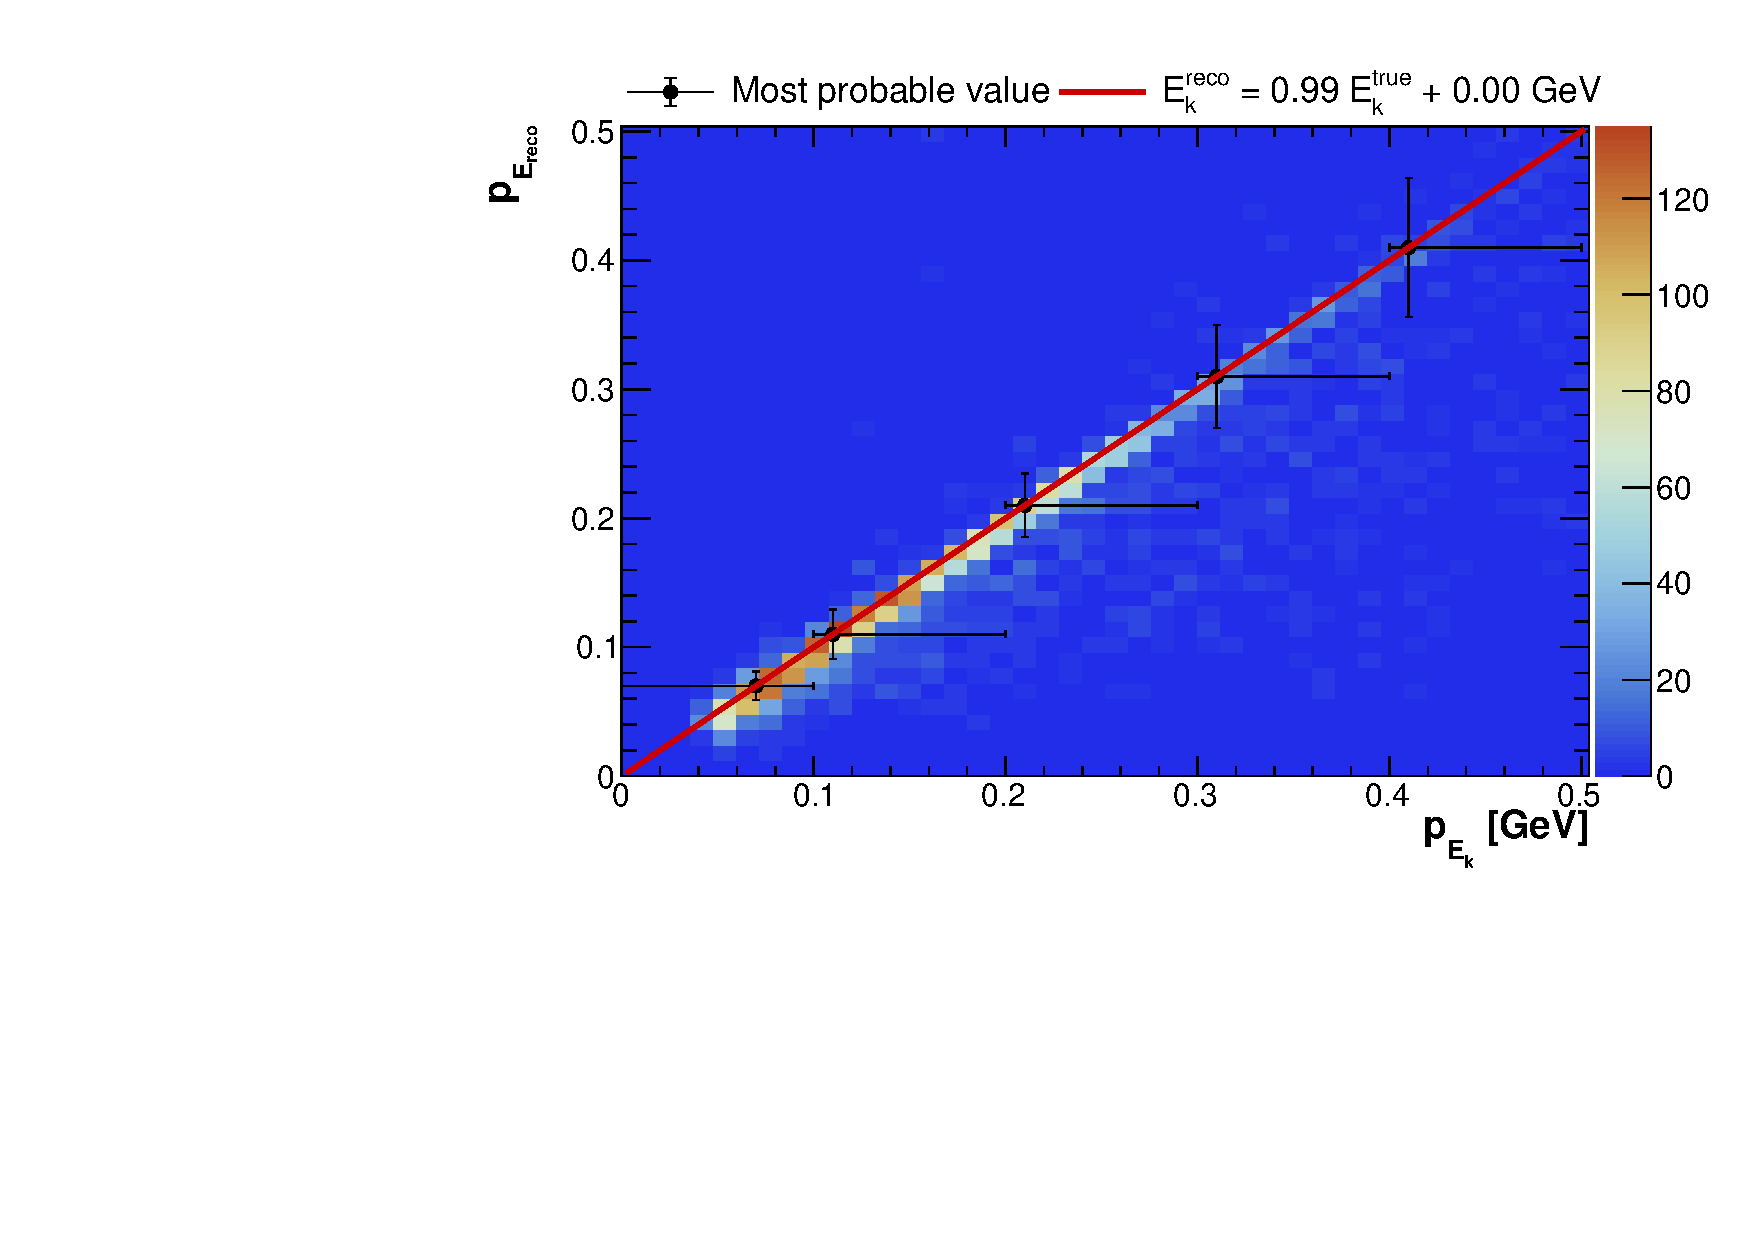
\includegraphics[width=0.65\columnwidth]{figures/pcalib.pdf}
\caption{Bi-dimensional histogram of true proton energy $E^{p}$ vs. reconstructed electron energy $E_{reco}^{p}$. Black points are obtained measuring the most probable value of the $E_{reco}^{p}$ distribution for each $E^{p}$ bin.}
\label{fig:pcalib}
\end{figure}


% \subsubsection{Neutrino Produced Hadronic Energy Reconstruction}

% \subsection{Neutrino Energy Reconstruction}
% Validation section should include: 
% Data/MC Agreement after precuts on all important variables
% Sideband Checks
% Corsika In-time vs BNB-ext
% Future Validation Studies

\section{Validation}

\subsection{Simulation/Data Comparisons}
In this section we will validate the background rejection cuts described in Section \ref{sec:bkg}. In particular, for each variable, we will show:
\begin{itemize}
\item the integral-normalized Monte Carlo distributions for the signal ($\nu_{e}$ CC0$\pi$-Np events), the cosmogenic background (cosmic, cosmic contaminated, and cosmic in-time), and the neutrino background ($\nu_{e}$ CC, beam intrinsic $\nu_{\mu}$, beam intrinsic NC, and dirt);

\item the POT-normalized Monte Carlo and data distributions, to verify the agreement of the simulation with the collected data.
\end{itemize}

\begin{description}
\item[Most energetic shower $E > 50~\mathrm{MeV}$.] The integral-normalized distributions in Figure \ref{fig:showere_integral} show that a large fraction of the cosmogenic and neutrino backgrounds have very low-energetic showers, while the signal component is almost constant. Figure \ref{fig:showere_pot} shows a good data/Monte Carlo agreement for this variable ($\chi^2 / \mathrm{n.d.f.} = 1.17$).

\begin{figure}[htbp]
\centering
  \begin{subfigure}{0.45\textwidth}
    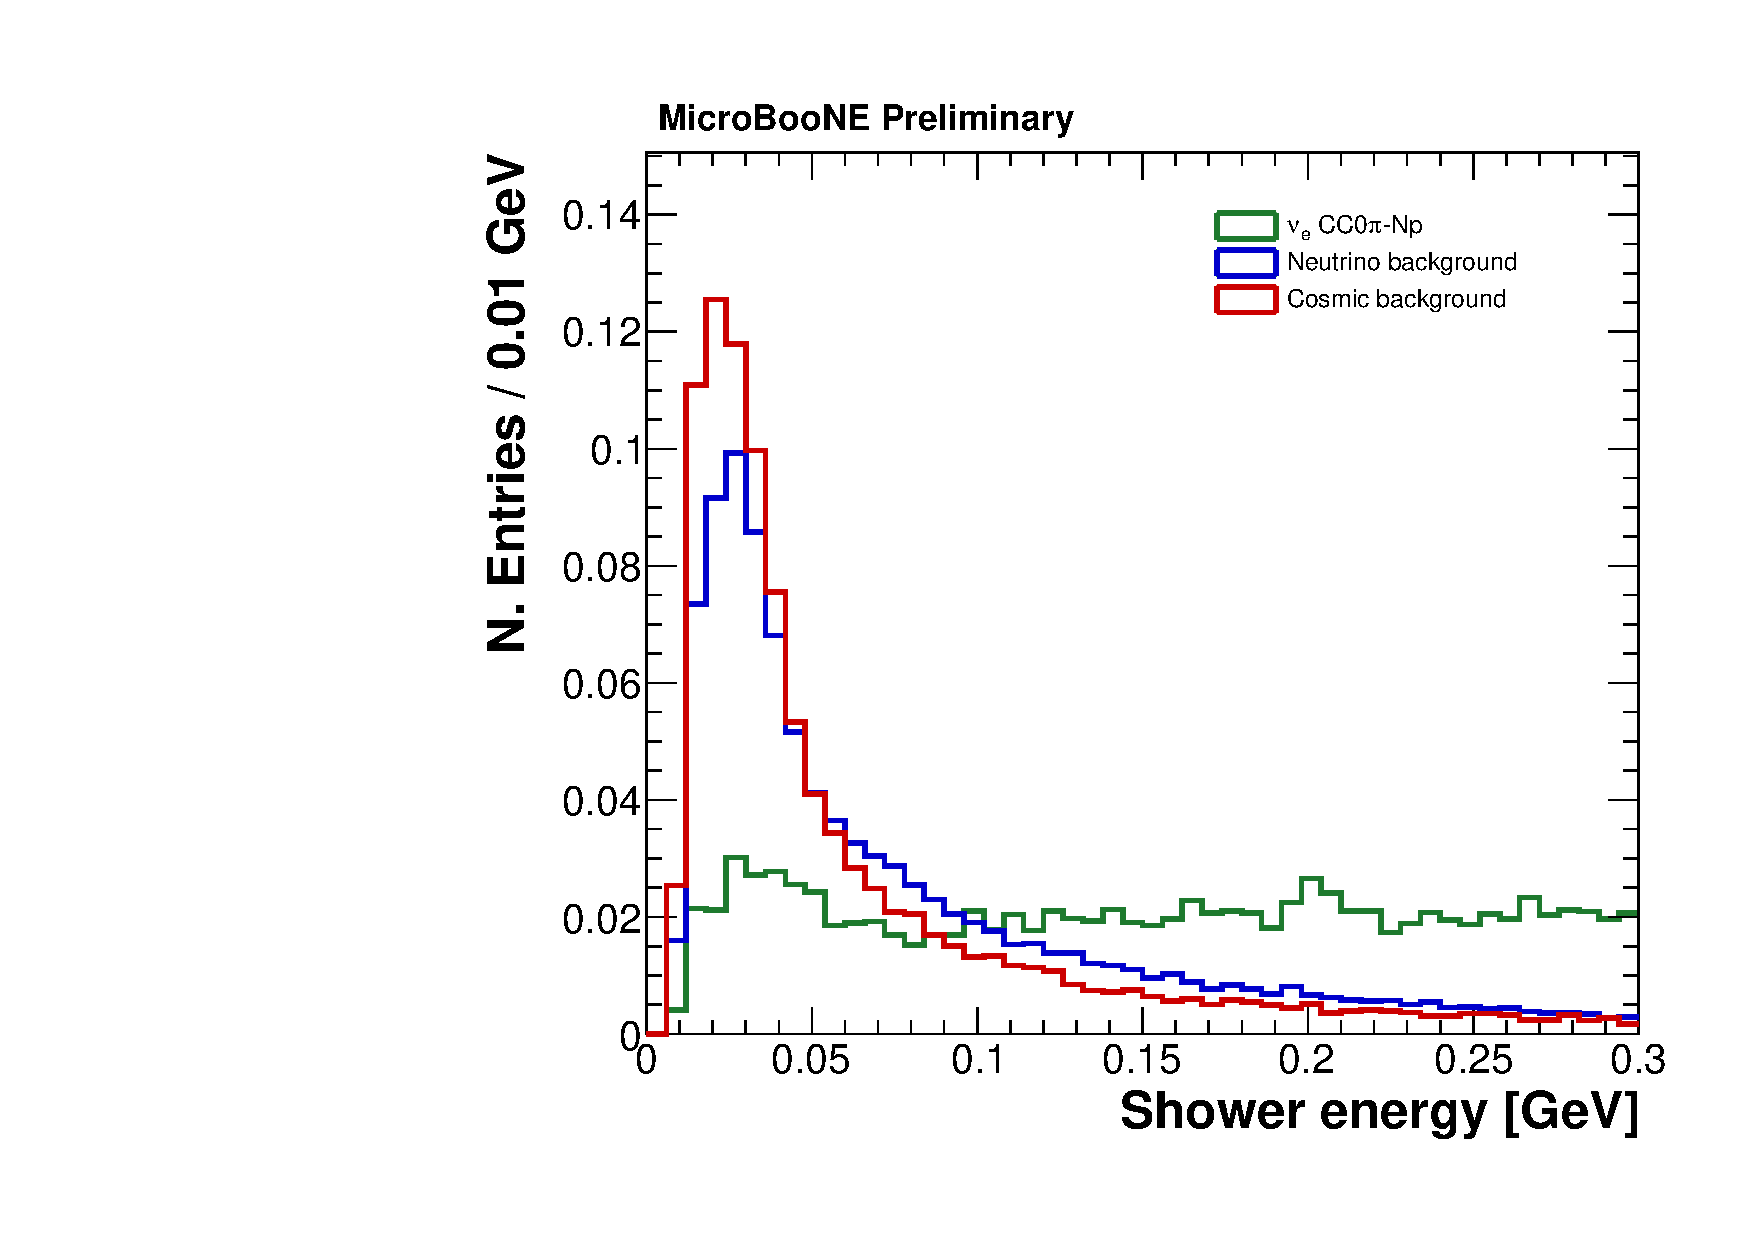
\includegraphics[width=\linewidth]{figures/h_shower_energy_norm.pdf}
    \caption{Integral normalized.} \label{fig:showere_integral}
  \end{subfigure}
    \begin{subfigure}{0.45\textwidth}
    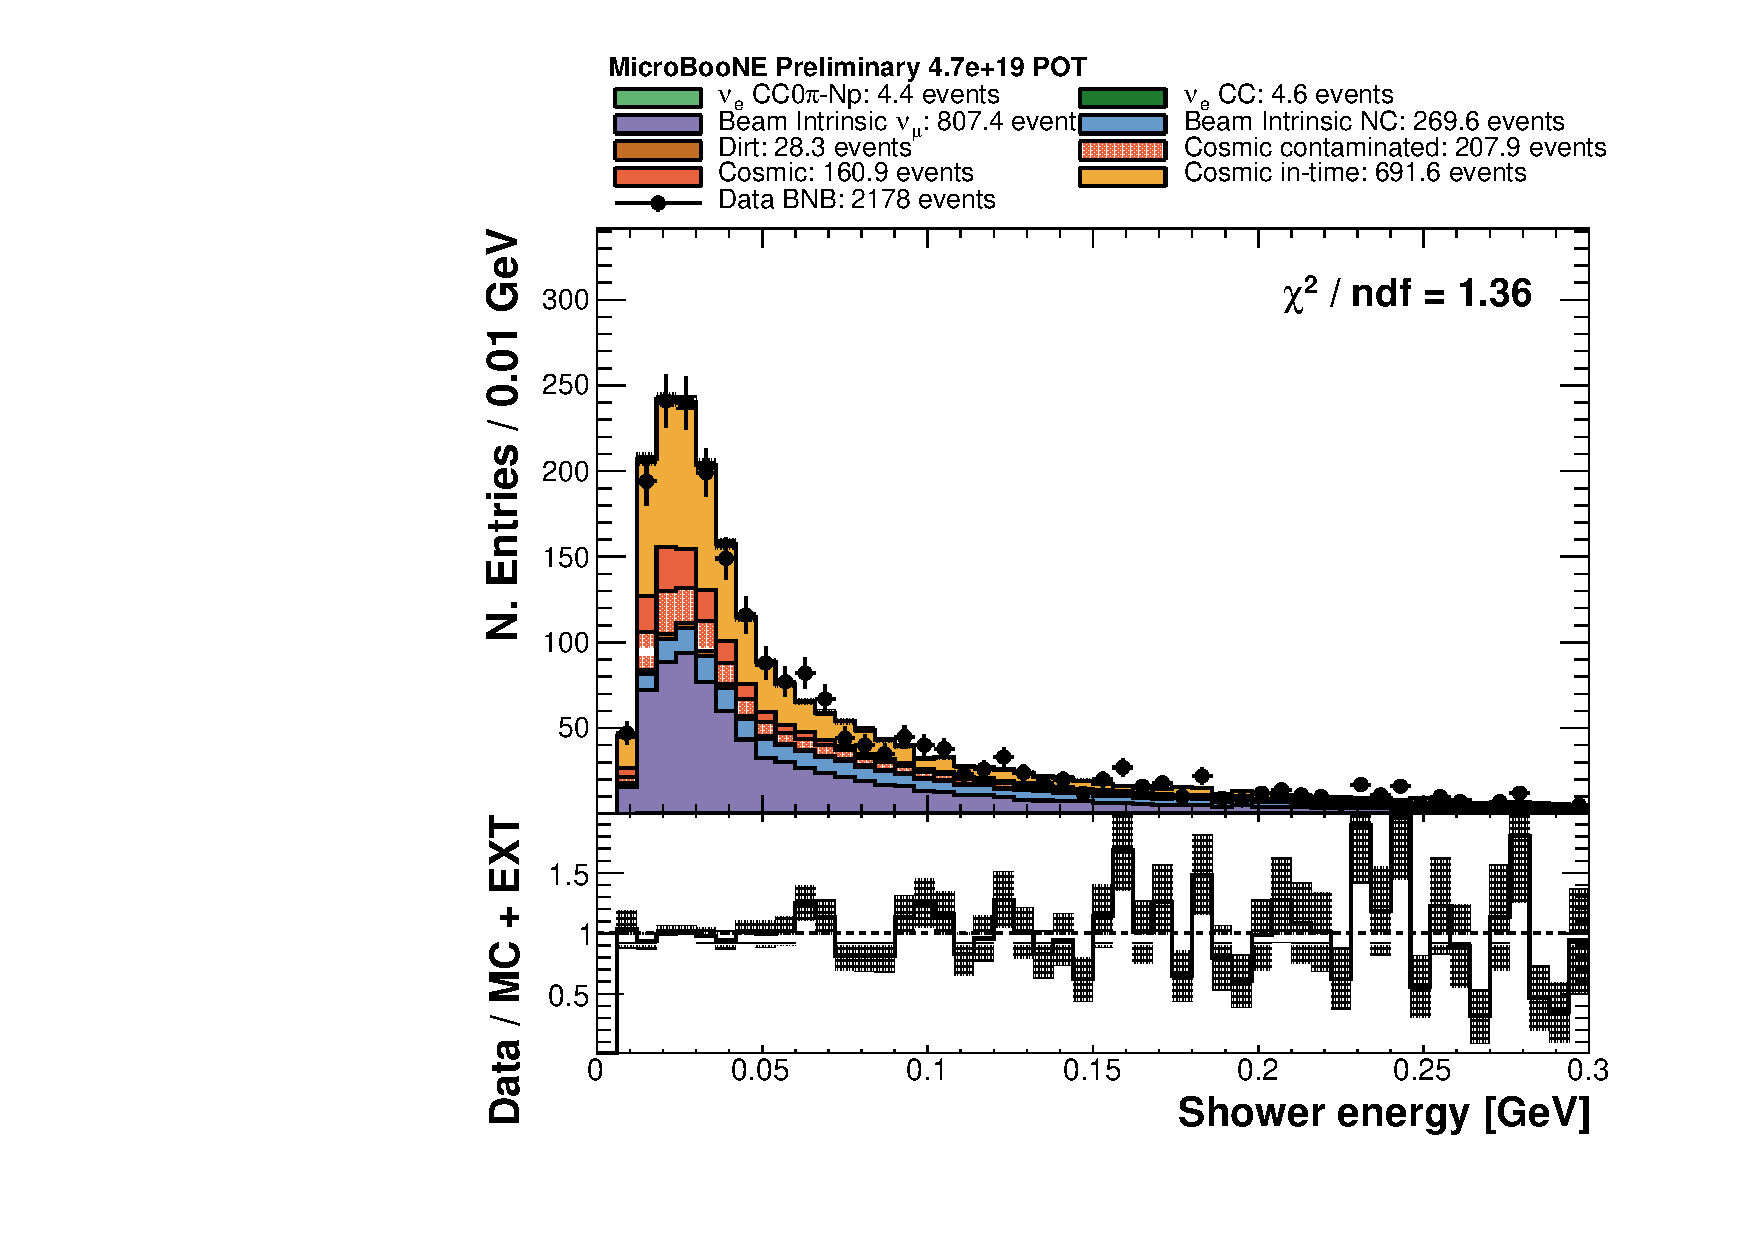
\includegraphics[width=\linewidth]{figures/h_shower_energy.pdf}
    \caption{POT normalized.} \label{fig:showere_pot}
  \end{subfigure}
  \caption{Integral and POT normalized distributions of the energy of the most energetic shower.}
\end{figure}

\item[Most energetic shower $1~\mathrm{MeV/cm} < dE/dx <3.2~\mathrm{MeV/cm}$.] Figure \ref{fig:dedx_integral} shows that the signal distribution is peaked around 2 MeV/cm, as expected. The beam intrinsic NC component has a second peak around 4 MeV/cm, mainly caused by $\pi^0\rightarrow2\gamma$ decays. The POT-normalized plot (Figure \ref{fig:dedx_pot}) shows a very good data/Monte Carlo agreement ($\chi^2 / \mathrm{n.d.f.} = 0.87$).

\begin{figure}[htbp]
\centering
  \begin{subfigure}{0.45\textwidth}
    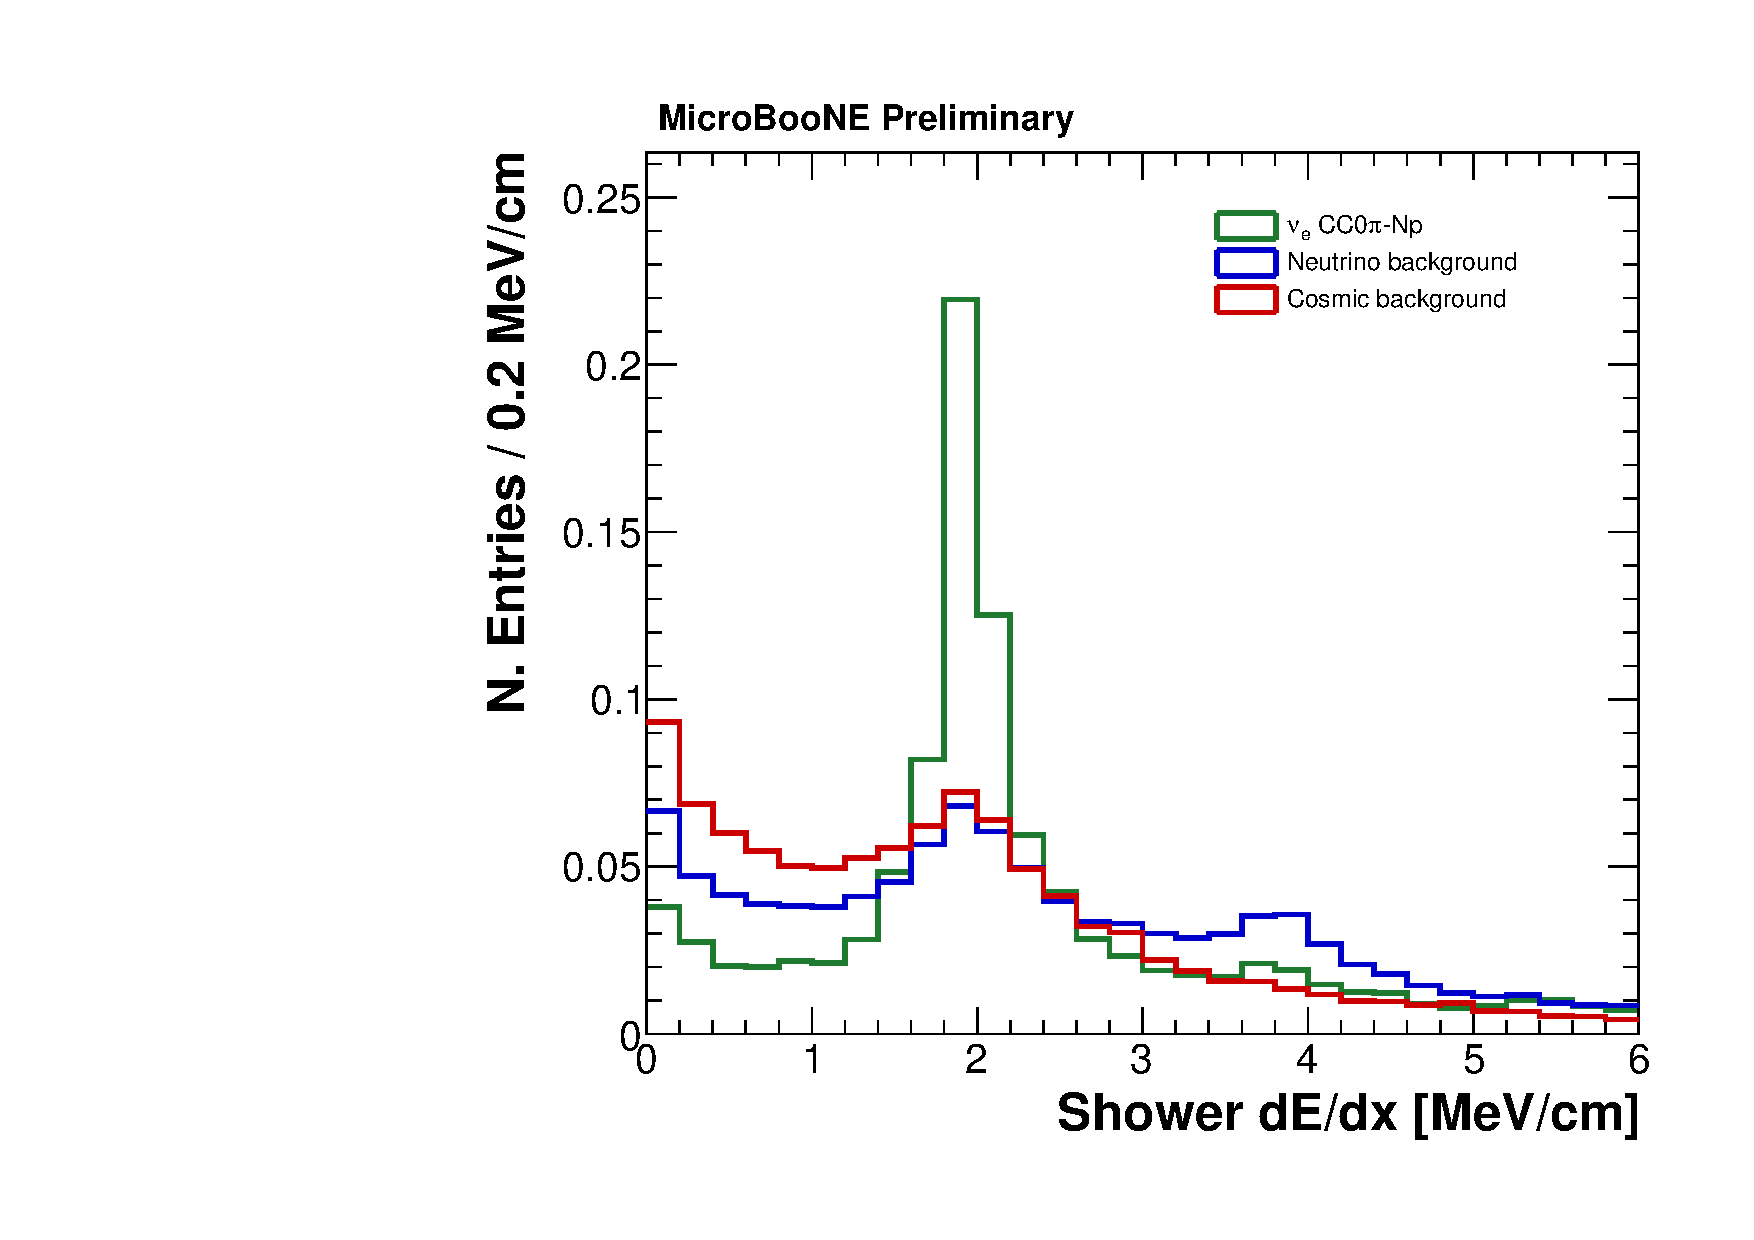
\includegraphics[width=\linewidth]{figures/h_dedx_norm.pdf}
    \caption{Integral normalized.} \label{fig:dedx_integral}
  \end{subfigure}
    \begin{subfigure}{0.45\textwidth}
    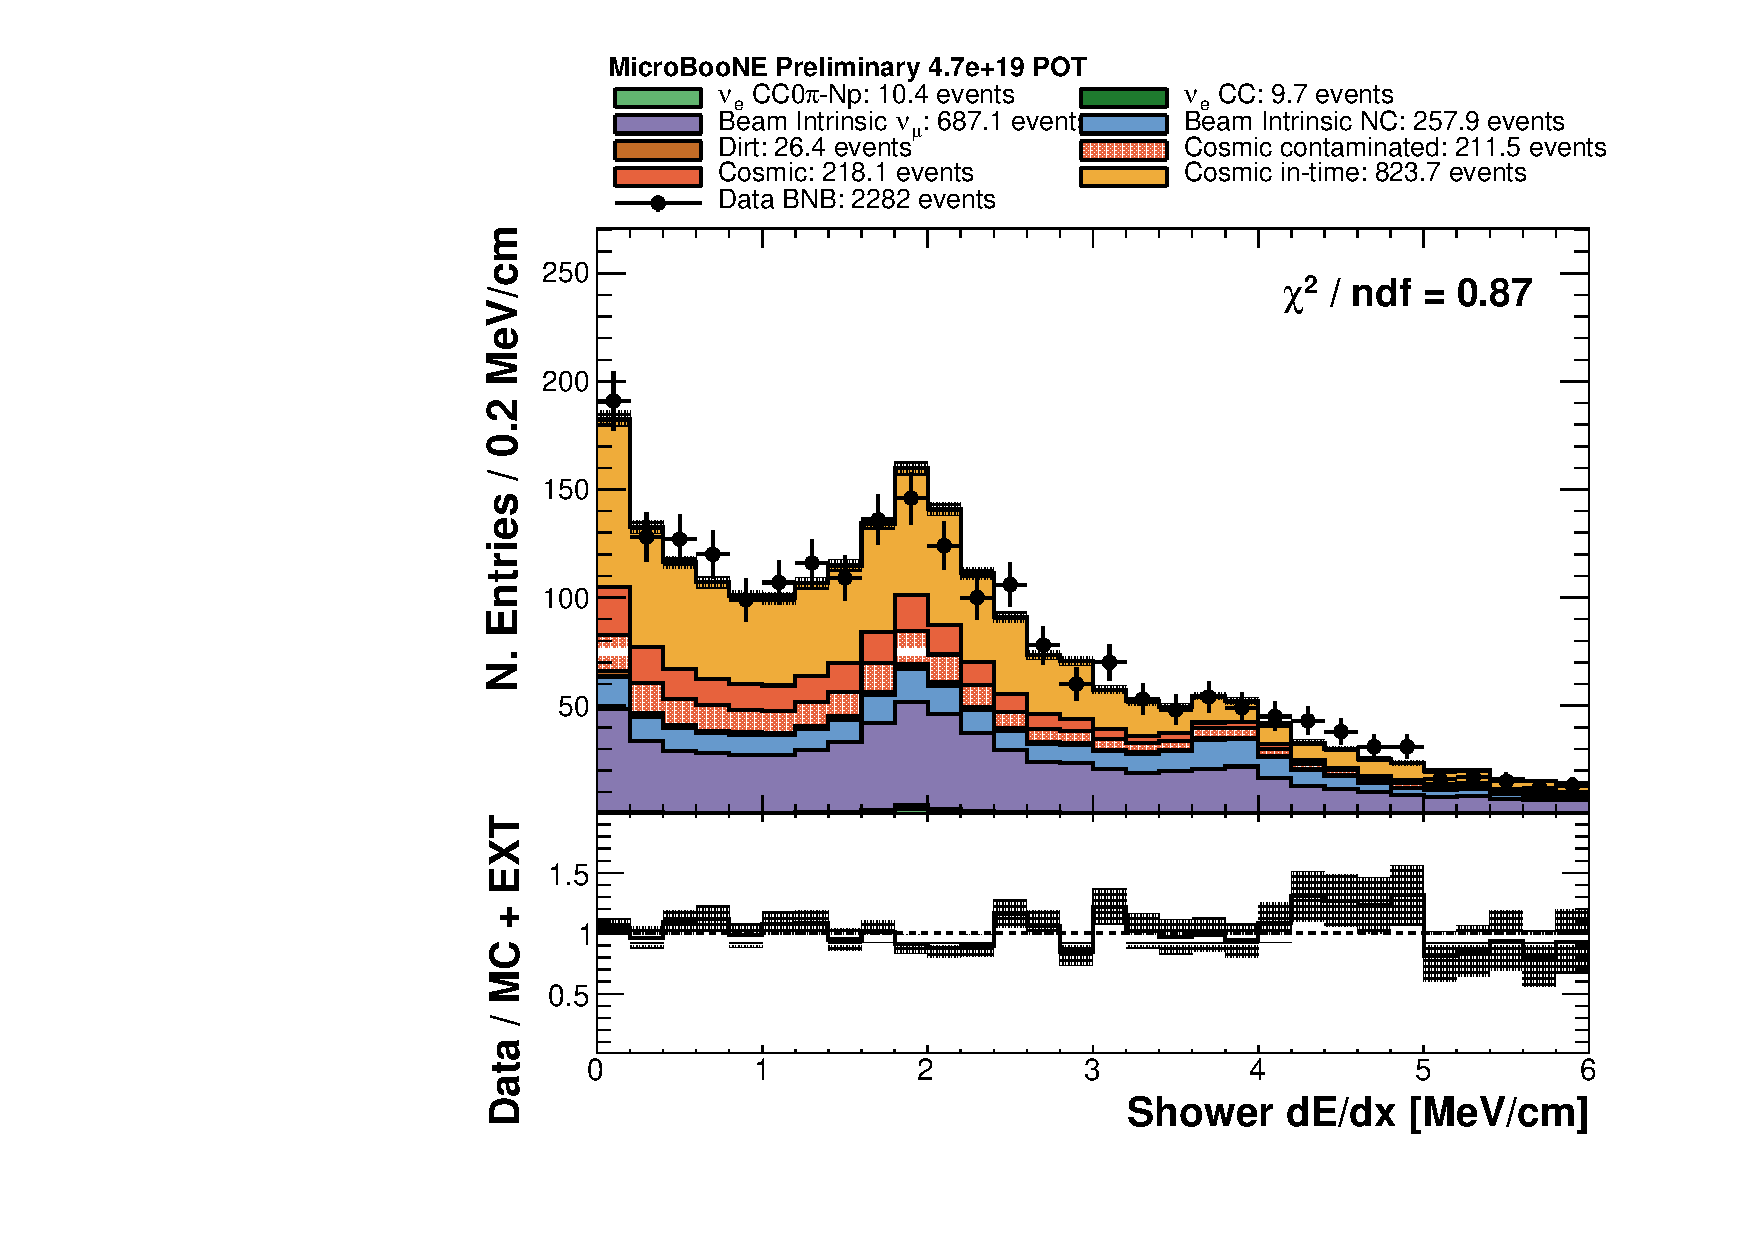
\includegraphics[width=\linewidth]{figures/h_dedx.pdf}
    \caption{POT normalized.} \label{fig:dedx_pot}
  \end{subfigure}
  \caption{Integral and POT normalized distributions of the $dE/dx$ of the most energetic shower.}
\end{figure}

\item[Track distance $d_{t} < 3$~cm.] Figure \ref{fig:track_norm} shows that the distributions of the distance between the start-point of the most proton-like track and the reconstructed neutrino vertex for signal and background are very similar. The cut $d_{t} < 3$~cm, then, mainly ensures that the event is well reconstructed. The data/Monte Carlo agreement in Figure \ref{fig:track_pot} is good, except for the first bin ($0~\mathrm{cm} < d_{t} < 0.5~\mathrm{cm}$), where we have a 10\% more Monte Carlo events than data. This small discrepancy could be explained by a slightly better vertex resolution in the simulation compared to data.

\begin{figure}[htbp]
\centering
  \begin{subfigure}{0.45\textwidth}
    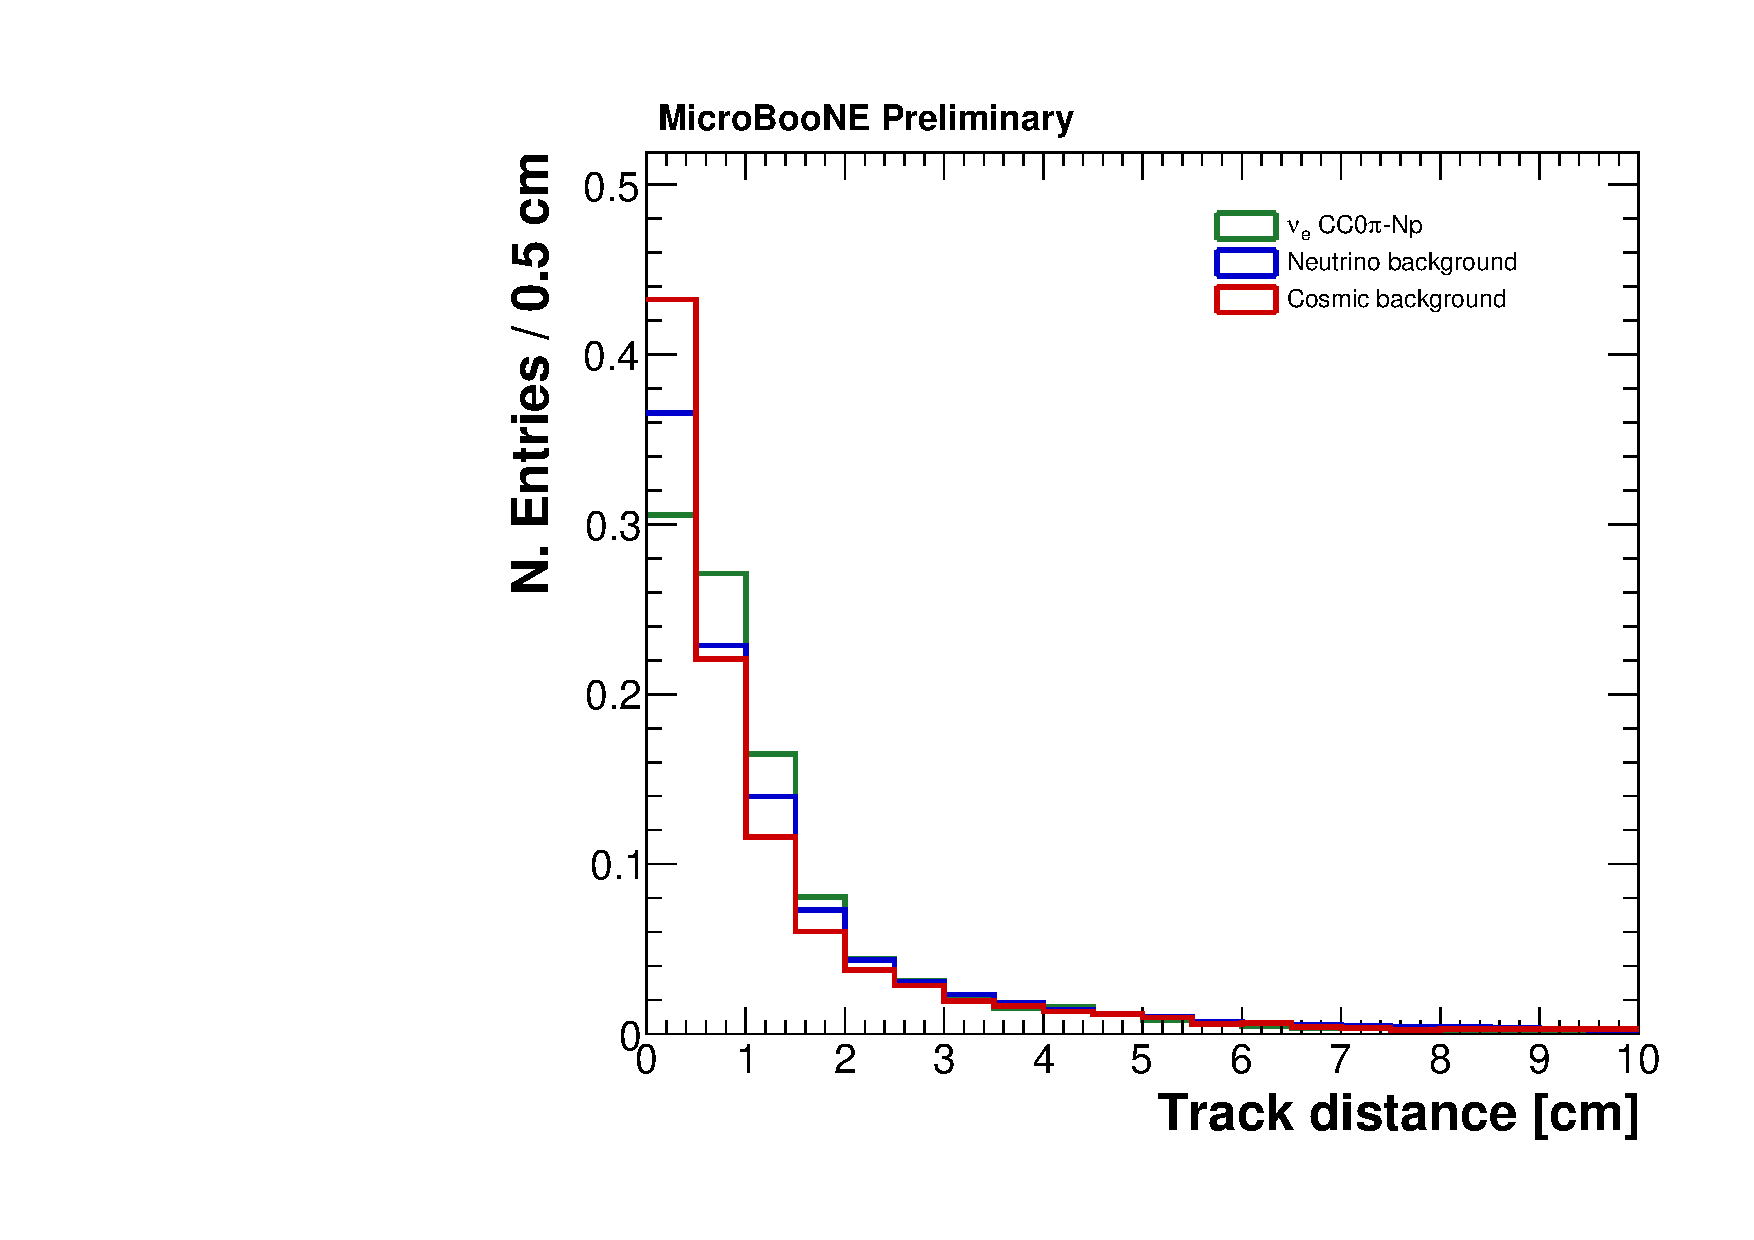
\includegraphics[width=\linewidth]{figures/h_track_distance_norm.pdf}
    \caption{Integral normalized.} \label{fig:track_norm}
  \end{subfigure}
    \begin{subfigure}{0.45\textwidth}
    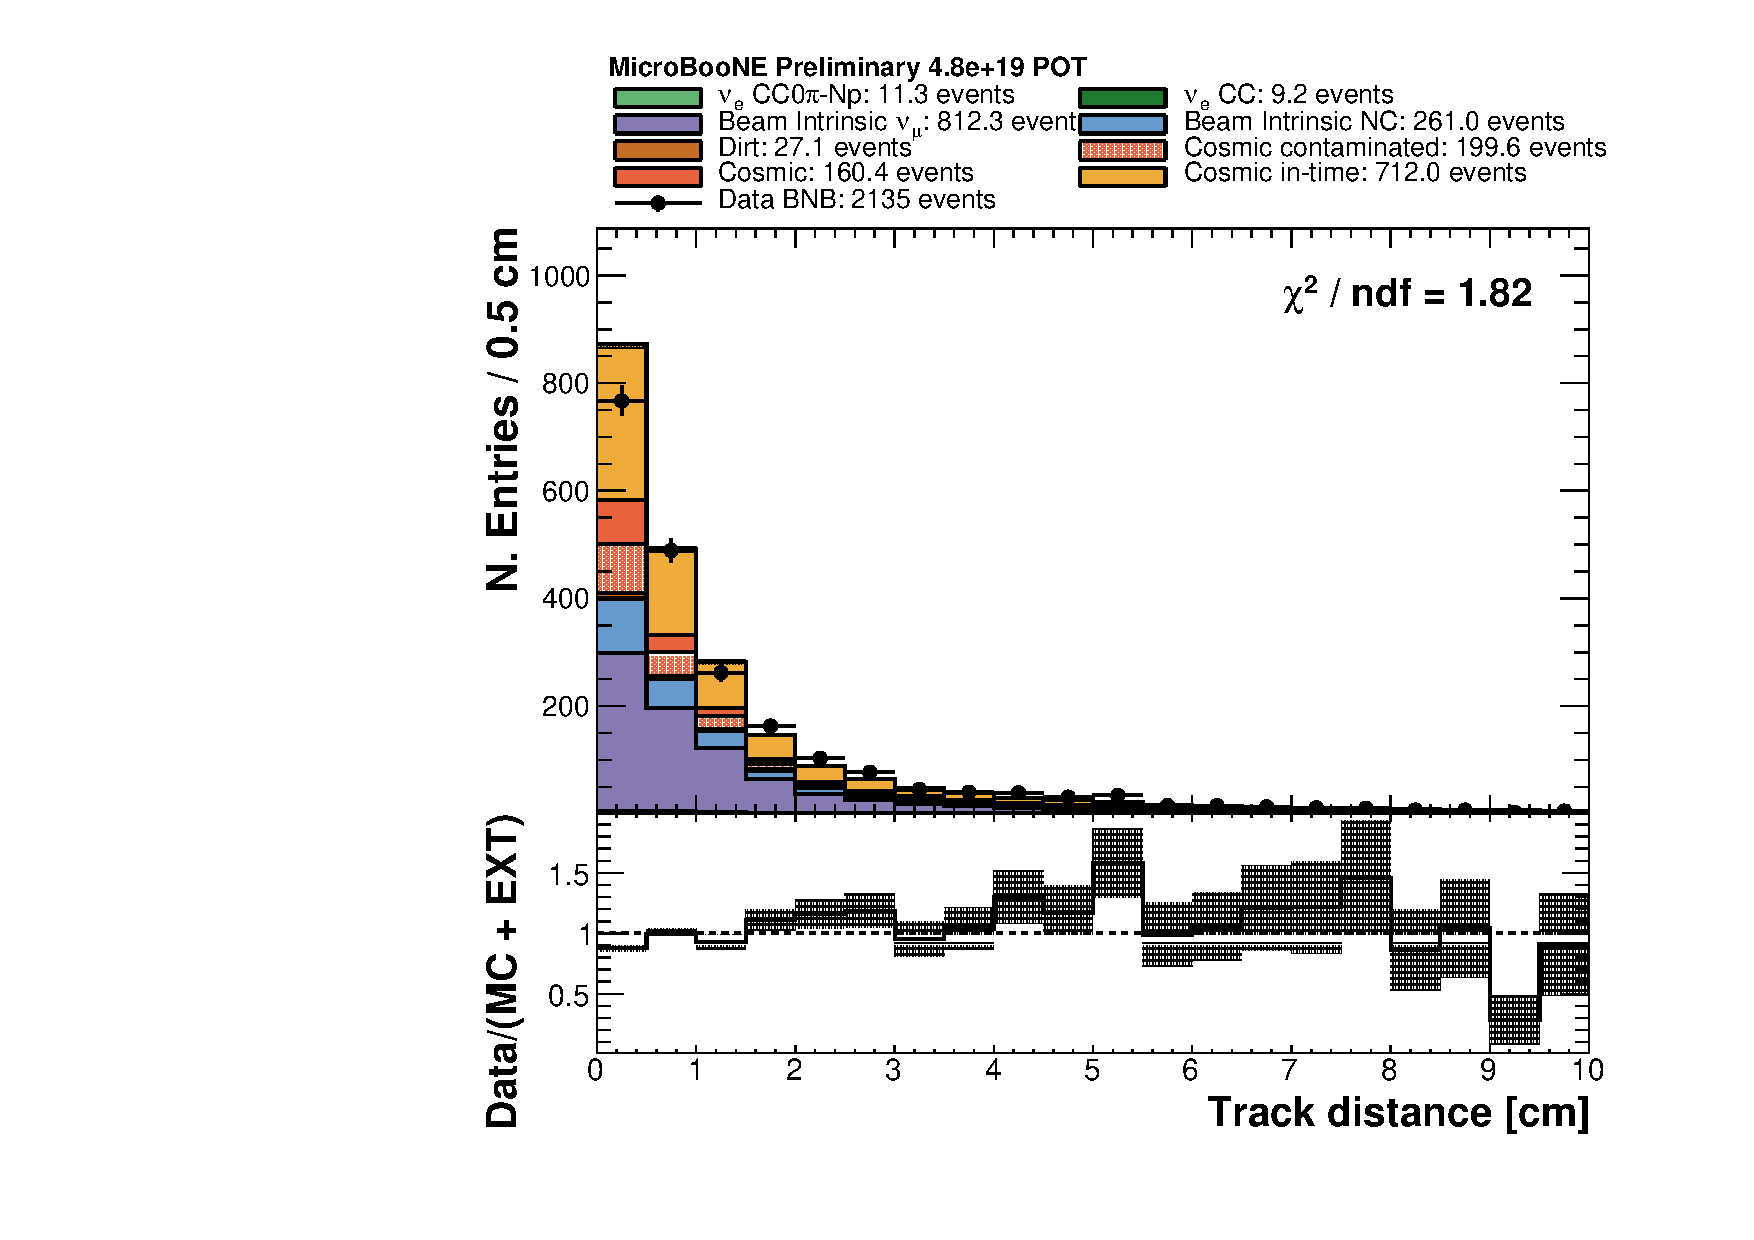
\includegraphics[width=\linewidth]{figures/h_track_distance.pdf}
    \caption{POT normalized.} \label{fig:track_pot}
  \end{subfigure}
  \caption{Integral and POT normalized distributions of the distance between the most proton-like track and the reconstructed neutrino vertex.}
\end{figure}

\item[Shower distance $d_{s} < 10$~cm.] Figure \ref{fig:shower_norm} shows the distributions of the distance between the start-point of the leading shower and the reconstructed neutrino vertex for signal and background events. As expected, background neutrino events have a larger tail than the signal events. However, the limited shower start-point spatial resolution does not allow us to place a stricter cut on this variable. The agreement between data and Monte Carlo shown in Figure \ref{fig:shower_pot} is good.

\begin{figure}[htbp]
\centering
  \begin{subfigure}{0.45\textwidth}
    \includegraphics[width=\linewidth]{figures/h_shower_distance_norm.pdf}
    \caption{Integral normalized.} \label{fig:shower_norm}
  \end{subfigure}
    \begin{subfigure}{0.45\textwidth}
    \includegraphics[width=\linewidth]{figures/h_shower_distance.pdf}
    \caption{POT normalized.} \label{fig:shower_pot}
  \end{subfigure}
  \caption{Integral and POT normalized distributions of the distance between the leading shower and the reconstructed neutrino vertex.}
\end{figure}

\item[Proton track BDT score $> -0.12$.] Figure \ref{fig:bdt_norm} shows the BDT score for the tracks in background and signal events, trained with the procedure described in Section \ref{sec:protbdt}. The cut at $-0.12$ allows to remove events with muon-like tracks. The data/Monte Carlo agreement shown in figure \ref{fig:bdt_pot} is good both in the signal region (high score) and in the background region (low score). The peak at -1 is caused by events with invalid $dQ/dx$ values (e.g. because of wrong vertex reconstruction).

\begin{figure}[htbp]
\centering
  \begin{subfigure}{0.45\textwidth}
    \includegraphics[width=\linewidth]{figures/h_dqdx_bdt_norm.pdf}
    \caption{Integral normalized.} \label{fig:bdt_norm}
  \end{subfigure}
    \begin{subfigure}{0.45\textwidth}
    \includegraphics[width=\linewidth]{figures/h_dqdx_bdt.pdf}
    \caption{POT normalized.} \label{fig:bdt_pot}
  \end{subfigure}
  \caption{Integral and POT normalized distributions of the BDT score of the reconstructed tracks.}
\end{figure}


\item[Track-shower angle $\mathrm{cos}\theta > -0.9$]. Figure \ref{fig:angle_integral} shows that there are, in proportion, more background events for events with a high angle between the most proton-like track and the most energetic shower. This cut allows to reject these events while also ensuring that the signal events are well-reconstructed. In fact, signal events with $\mathrm{cos}\theta \approx 1$ have almost always an electron shower reconstructed as a track-like object in the first part. The agreement shown in Figure \ref{fig:angle_pot} is good.

\begin{figure}[htbp]
\centering
  \begin{subfigure}{0.45\textwidth}
    \includegraphics[width=\linewidth]{figures/h_track_shower_angle_norm.pdf}
    \caption{Integral normalized.} \label{fig:angle_integral}
  \end{subfigure}
    \begin{subfigure}{0.45\textwidth}
    \includegraphics[width=\linewidth]{figures/h_track_shower_angle.pdf}
    \caption{POT normalized.} \label{fig:angle_pot}
  \end{subfigure}
  \caption{Integral and POT normalized distributions of the angle between the most proton-like track and the most energetic shower.}
\end{figure}

\item[Most energetic shower opening angle $1^{\circ} < \theta < 20^{\circ}$]. The distributions of the opening angle $\theta$ of the most energetic shower for neutrino and cosmic background events have a larger tail than the signal events, as shown in Figure \ref{fig:open_integral}. The cut $1^{\circ} < \theta < 20^{\circ}$ helps rejecting some background events, while removing only a small fraction of mainly high-energy signal events. Figure \ref{fig:open_pot} shows a good data/Monte Carlo agreement.

\begin{figure}[htbp]
\centering
  \begin{subfigure}{0.45\textwidth}
    \includegraphics[width=\linewidth]{figures/h_shower_open_angle_norm.pdf}
    \caption{Integral normalized.} \label{fig:open_integral}
  \end{subfigure}
    \begin{subfigure}{0.45\textwidth}
    \includegraphics[width=\linewidth]{figures/h_shower_open_angle.pdf}
    \caption{POT normalized.} \label{fig:open_pot}
  \end{subfigure}
  \caption{Integral and POT normalized distributions of the opening angle of the most energetic shower.}
\end{figure}

\item[Most proton-like track length $L < 80~\mathrm{cm}$]. Both neutrino and cosmic background events have on average longer reconstructed tracks than signal events, as shown in Figure \ref{fig:length_norm}. The cut $L < 80~$cm increases the signal purity without significantly decreasing the signal efficiency. The agreement between data and Monte Carlo distributions is good (Figure \ref{fig:length_pot}).

\begin{figure}[htbp]
\centering
  \begin{subfigure}{0.45\textwidth}
    \includegraphics[width=\linewidth]{figures/h_track_length_norm.pdf}
    \caption{Integral normalized.} \label{fig:length_norm}
  \end{subfigure}
    \begin{subfigure}{0.45\textwidth}
    \includegraphics[width=\linewidth]{figures/h_track_length.pdf}
    \caption{POT normalized.} \label{fig:length_pot}
  \end{subfigure}
  \caption{Integral and POT-normalized distributions of the length of the most proton-like track.}
\end{figure}

\end{description}

\subsection{Side-bands checks}
\subsubsection{Introduction}
In this section we will show the agreement between data and Monte Carlo for selected samples mostly orthogonal to our $\nu_{e}$ CC0$\pi$-Np signal. In particular, some of the background cuts described in Section \ref{sec:bkg} will be inverted or removed in order to enhance different background components.

\subsubsection{Photon-enhanced reverse cuts}
It is possible to enhance the neutral-current component (defined as beam intrinsic NC in our analysis) by (1) inverting the cut on the shower $dE/dx$, (2) removing the requirement on the shower opening angle, and (3) removing the cut on the track distance. The $dE/dx$ of the most energetic shower must be within 3.2~MeV/cm and 5~MeV/cm to ensure that the electromagnetic cascade was initiated by a photon. Removing the cut on the shower opening angle allows to include events where two photon showers from a $\pi^{0}\rightarrow 2\gamma$ decay are reconstructed as a single object. The cut on the track distance is removed to increase the size of the sample.
Thus, our final sample will mainly contain NC$\pi^{0}$, with a small contamination of $\nu_{\mu}$ CC$\pi^{0}$ events where the muon track was tagged as a proton-like track.

Figure \ref{fig:photon} shows a good agreement between data and Monte Carlo for the reconstructed energy spectrum of the photon-enhanced event spectrum.

\begin{figure}[htbp]
\centering
  \includegraphics[width=0.65\linewidth]{figures/nc_reco.pdf}
  \caption{Reconstructed energy spectrum of the events selected with the photon-enhanced reverse cuts.}\label{fig:photon}
\end{figure}

\subsubsection{CC \texorpdfstring{$\nu_{\mu}$}{numu}-enhanced reverse cuts}
It is possible to enhance the presence of the CC $\nu_{\mu}$ background (defined as beam intrinsic $\nu_{\mu}$ in our analysis) by (1) requiring a minimum track length, (2) removing the cut on the proton BDT, and (3) requiring that the event is selected by the auxiliary \texttt{UBXSec} module. 
A CC $\nu_{\mu}$ event has, by definition, a muon in the final state: as such, requiring a track length larger than 20~cm and removing the cut on the proton BDT decreases our muon-rejection power. The goal of the auxiliary \texttt{UBXSec} module is to select CC $\nu_{\mu}$ events, so instead of vetoing those events as described in \ref{sec:numu}, we invert this requirement by allowing only the events selected by \texttt{UBXSec}.

Figure \ref{fig:numu_inverted} shows a good agreement between data and Monte Carlo for the reconstructed energy spectrum of the CC $\nu_{\mu}$-enhanced event spectrum.

\begin{figure}[htbp]
\centering
  \includegraphics[width=0.65\linewidth]{figures/numu_reco.pdf}
  \caption{Reconstructed energy spectrum of the events selected with the CC $\nu_{\mu}$-enhanced reverse cuts.}\label{fig:numu_inverted}
\end{figure}

\subsection{Future Validation Studies}

\subsubsection{CORSIKA in-time / EXT comparison}
In order to validate the cosmic-ray components of our selected events it is possible to compare simulated events with a CORSIKA cosmic ray producing a flash in the optical system during the beam-gate window and the data EXT sample. 
In this way we will be able to check if the distributions of the variables we use (e.g. shower energy, shower $dE/dx$) have or not a good agreement between the simulation and a well-understood set of data events. 
It will help validating the cosmic background components and also the energy and $dE/dx$ reconstruction procedures.

\subsubsection{Data/MC Comparisons with NuMI}
It is possible to run this analysis on the complementary NuMI dataset. The NuMI neutrino beam has a higher energy than the BNB (the first one is created from 120 GeV protons hitting on a carbon target, while the second one from 8 GeV protons on beryllium). NuMI has also a higher beam intrinsic $\nu_{e}$ component than BNB (5\% vs. 0.5\%), as shown in Figure \ref{fig:numibeam}. Even if off-axis, MicroBooNE will then receive $\sim2500$ $\nu_{e}$ interactions per year. 
As such, a study of the events selected in the NuMI dataset is of fundamental importance to validate the $\nu_{e}$ CC0$\pi$-Np selection algorithm in a different energy region, where the effect of the MiniBooNE low-energy excess should be negligible.

\begin{figure}[htbp]
\centering
  \begin{subfigure}{0.45\textwidth}
    \includegraphics[width=\linewidth]{figures/numi.pdf}
    \caption{NuMI beam flux.} 
  \end{subfigure}
    \begin{subfigure}{0.45\textwidth}
    \includegraphics[width=\linewidth]{figures/bnb.pdf}
    \caption{BNB beam flux.} 
  \end{subfigure}
  \caption{NuMI and BNB neutrino fluxes for each neutrino and antineutrino component.}\label{fig:numibeam}
\end{figure}


% Show distributions for loose cuts, 5e19 data/MC comparison
% Aggressive cuts, 6.6e20 Projection
% Current efficiency and purity plots as a function of energy

\section{Electron-Like Event Distributions}\label{sec:electron_like}
\subsection{Reconstructed energy spectrum}
The reconstructed energy spectrum of the selected events after the application of the background-rejection cuts is shown in Figure \ref{fig:spectrum_after}. It corresponds to the sum of the reconstructed energies of the shower-like objects, as described in Section \ref{sec:showerenergy}, and the reconstructed energies of the track-like objects, as described in Section \ref{sec:protonenergy}. 

\begin{figure}[htbp]
\centering
  \includegraphics[width=0.65\linewidth]{figures/h_fixed_energy_after.pdf}
    \caption{Reconstructed energy spectrum of the selected events after the background-rejection cuts.}\label{fig:spectrum_after}

\end{figure}


The final number of selected data events in the unblinded data sample is 21, corresponding to a MicroBooNE exposure of \num{4.84e19} POT. These events have been hand-scanned: Figure \ref{fig:evds} shows the event displays of two $\nu_{e}$-like selected data events.


The data BNB distribution is in good agreement with the stacked Monte Carlo + EXT distributions, both in normalization (the integral ratio is 1.03) and in shape ($\chi^2 /\mathrm{n.d.f.} = 0.68$). 
%The signal component ($\nu_{e}$ CC0$\pi$-Np events) represents now the largest component among the event categories with 4.1 events. 

\subsection{Efficiency and purity}
It is now possible to calculate the efficiency and the purity of our $\nu_{e}$ CC0$\pi$-Np selection after the background-rejection cuts, as defined in Section \ref{sec:eff}. The background-rejection cuts were aimed to improve the significance of the $\nu_{e}$ CC0$\pi$-Np events in our sample. Thus, the efficiency decreases, from 41.1\% to 14.3\%, since the cuts will eventually remove also some signal events, but the purity increases by a factor of $\sim50$, from 0.5\% to 23.9\%. Figure \ref{fig:effafter} shows the efficiency as a function of the true neutrino energy and the purity as a function of the reconstructed energy, before and after the background rejection cuts. 

\begin{figure}
  \begin{subfigure}{0.48\textwidth}
    \includegraphics[width=\linewidth]{figures/eff_after.pdf}
    \caption{Efficiency} 
  \end{subfigure}
    \begin{subfigure}{0.48\textwidth}
    \includegraphics[width=\linewidth]{figures/purity_after.pdf}
    \caption{Purity} 
  \end{subfigure}
  \caption{Left: $\nu_{e}$ CC$0\pi$-Np reconstruction efficiency as a function of the true $\nu_{e}$ energy before and after the background-rejection cuts. Right: $\nu_{e}$ CC$0\pi$-Np purity as a function of the reconstructed energy before and after the background-rejection cuts.}
  \label{fig:effafter}
\end{figure}

Table \ref{tab:effafter} shows the efficiency and the number of events selected for each event category before and after the background-rejection cuts. In particular, we are able to reject the 99.5\% of the neutrino background and the 
99.996\% of the cosmogenic background, while retaining a 14.3\% $\nu_{e}$ CC0$\pi$-Np efficiency.

\begin{table}[htbp]
   \centering
   \begin{tabular}{llrrrrrrrr}
     \toprule
     Category & \phantom{a} & Generated & \phantom{a} & Selected & \phantom{a} & After cuts & \phantom{a} & Efficiency\\
     \midrule

     $\nu_{e}$ CC0$\pi$-Np       & & 34.8     & & 14.3   & & 4.9   & & 14.3\%\\
     $\nu_{e}$ CC                & & 35.7     & & 13.2   & & 1.6   & & 4.5\%\\
     Beam intrinsic $\nu_{\mu}$  & & 11337.4  & & 918.3  & & 5.0   & & 0.044\%\\
     Beam intrinsic NC           & & 3633.9   & & 342.2  & & 3.3   & & 0.09\%\\
     Dirt                        & & 2609.5   & & 37.1   & & 0.3   & & 0.01\%\\
     Cosmic in-time              & & 135377.2 & & 1151.6 & & 3.5   & & 0.003\%\\
     Cosmic contaminated         & & -        & & 260.7  & & 1.1   & & 0.4\%\\
     Cosmic                      & & -        & & 233.3  & & 0.9   & & 0.4\%\\

     \bottomrule
   \end{tabular}
   \caption{Summary of the selection algorithm results, showing the contribution of each event category, for a MicroBooNE exposure of \num{4.84e19} POT.}\label{tab:effafter}
\end{table}

\begin{figure}[htbp]
\centering
  \begin{subfigure}{0.7\textwidth}
  \includegraphics[width=\linewidth]{figures/data1.png}
    \caption{Event 1515, Subrun 30, Run 5328}
\end{subfigure}
  \begin{subfigure}{0.7\textwidth}	
  \includegraphics[width=\linewidth]{figures/data2.png}
  \caption{Event 31, Subrun 0, Run 5513}
\end{subfigure}

  \caption{Event displays of the collection plane of two $\nu_{e}$-like data events present in our sample after the background-rejection cuts. The gaps are caused by the presence of missing or unresponsive wires. The red lines correspond to reconstructed track-like objects and the green cones correspond to reconstructed shower-like objects. }
  \label{fig:evds}
\end{figure}
% Outlook section

\section{Outlook}

The analysis presented here is at a mature stage, but certainly not in its final for publication.  In this section, we will outline anticipated future improvements we plan to make and complementary analyses that will directly impact this result.

\subsection{Future Improvements}
\subsubsection{Track/Shower Classification}

The preceding sections showed there is significant disagreement in the track-like/shower-like classification of objects when comparing data to Monte Carlo.  In particular, the number of showers in data is higher than the number of showers in Monte Carlo, as shown in Section~\ref{sec:reclass}.  A mask is presented there to improve data/Monte Carlo agreement, by reclassifying (1) small shower-like objects as tracks based on their angular separation from the leading shower, and (2) track-like objects as showers if they are within the cone of the leading shower.  

The mask, unfortunately, is not a real solution.  Because of the difference in energy reconstruction between tracks and showers (range-based for tracks, calorimetric for showers), it's critical to the neutrino energy reconstruction to correctly identify the particles in an interaction.  Currently, we have simply ensured that the level of mis-identification between data and Monte Carlo is matched.

In principle, the track/shower misidentification issue is a collaboration-wide problem to be addressed for MCC9.  To this end, we anticipate trying short-term techniques such as BDT/SVM classifiers for TPC objects to improve classification in MCC8. Pandora itself uses an SVM classifier for track/shower separation, with good performance on Monte Carlo. By examining this training and including a data driven training set, we could improve performance on data as well. More ambitious updates from Pandora for MCC9, with the inclusion of improved signal processing and 2D deconvolution, fall under the realm of Pandora development.  We look forward to contributing to those discussions by validating and iterating on the improvements with the Pandora team.

\subsubsection{Neutrino Vertexing and Shower Splitting}

Another issue uncovered in the reconstruction of $\nu_{e}$ events is the splitting of electromagnetic showers and misplacement of the vertexes. 
Figure~\ref{fig:evd_2showers} shows an example of this problem.  

\begin{figure}[htbp]
\centering
  \includegraphics[width=0.7\linewidth]{figures/splitshower.png}
  \caption{Simulated event displays of the collection plane of a $\nu_{e}$ CC0$\pi$-Np event with the electron shower being split into several shower-like objects.}
  \label{fig:evd_2showers}
\end{figure}

For the low-energy excess analyses, this presents a problem for two reasons.  First, it introduces non-$\nu_{e}$ CC0$\pi$-Np events into the selected sample, since the track-like segment of an electromagnetic shower is reconstructed like a proton. Second, the splitting of a shower into multiple shower objects leads to a decreased ability to reject multi-shower events like $\pi^0\rightarrow2\gamma$ decays.

Improved clustering - particularly shower clustering - allows us to apply shower multiplicity cuts to reject background events with less aggressive cuts on the electron-like signal.

\subsubsection{Cosmic tagging with the Cosmic-ray Tagger}

In the final event distributions in Section~\ref{sec:electron_like}, the cosmic background is a sub-dominant background, due to the ability to reject these events with kinematic cuts.  However, as seen in Section~\ref{sec:numu}, the dominant source of events passing the pre-selection is cosmic-ray interactions.  The Cosmic-ray Tagger (CRT) offers several ways to reject these events at the pre-selection stage.  First, a coincidence veto of in-time flashes in the PMTs and CRT would allow us to reject a significant background of in-time cosmic events.  There is some danger that neutrino interactions are also vetoed by this coincidence, but that is unlikely for $\nu_{e}$ events - most particles that exit the TPC and can hit the CRT are muons.

Additionally, for events where an out-of-TPC neutrino interaction creates a flash in time with the beam, but a cosmic interaction is matched to that flash, the CRT can also be useful.  TPC-to-CRT matching of muon tracks can mitigate this background by flagging a TPC Pandora neutrino candidate object, and allowing us to reject out-of-time cosmic rays matched to an in-time, out-of-TPC neutrino flash.

\subsection{Complementary Analyses}

While many MicroBooNE analyses benefit this low-energy excess analysis, several in particular are directly complementary to this analysis and the coherence of their development is important to the future progress of this analysis.

\subsubsection{\texorpdfstring{$\nu_{\mu}$}{numu} Inclusive Selection}

All MicroBooNE low-energy excess searches benefit greatly from the constraint of flux, cross sections, and perhaps detector systematics by performing a joint measurement of $\nu_\mu$ and $\nu_e$ selections. In particular, the inclusive CC $\nu_\mu$ cross-section measurement described in \cite{ubxsec} also allows us to remove some $\nu_\mu$ mis-reconstructed as $\nu_e$ CC0$\pi$-Np candidates.

\subsubsection{Single Electron Inclusive Search}

Since final state interactions of neutrino's on liquid argon are not yet completely understood, a complementary $\nu_e$ CC inclusive search is ongoing. The inclusive channel is expected to be less sensitive to uncertainties in the neutrino interaction models. By not requiring the a proton, theoretically, higher sensitivities at low energy are possible. Meanwhile, reconstruction and identification problems concerning protons are less important. Both the $\nu_e$ CC0$\pi$-Np and $\nu_e$ CC inclusive will share the same cosmic rejection and optical selection. The inclusive search employs particle identification using the boosted decision classifier method for electrons and muons. Reconstructed objects are tagged as electron neutrino's based on classifier using the particle identification as its input. The BNB $\nu_e$ CC inclusive search will also be compared with the ongoing NUMI $\nu_e$ CC inclusive measurement.

\subsection{Background Rejection Improvements}
The cuts described in Section \ref{sec:bkg} have two main goals: (1) ensure that the selected events are well-reconstructed, and (2) reject the background events. However, the values of each cut, even if meaningful and justified, are not optimized to the significance of the $\nu_e$ CC0$\pi$-Np component in the sample. Doing that would have left us with too few data events, making the validation of the energy spectrum shown in Section \ref{sec:electron_like} impossible. 


\section{Conclusion}
\todo{Write the conclusion}

\newpage

\begin{thebibliography}{99}

\bibitem{miniboone}
  A.~A.~Aguilar-Arevalo {\emph{et al.}} [MiniBooNE Collaboration],
  ``Unexplained Excess of Electron-Like Events From a 1-GeV Neutrino Beam,''
  Phys.\ Rev.\ Lett.\  \textbf{102} (2009) 101802
  doi:10.1103/PhysRevLett.102.101802
  \href{https://arxiv.org/abs/0812.2243}{\texttt{[arXiv:0812.2243 [hep-ex]]}}.
  %%CITATION = doi:10.1103/PhysRevLett.102.101802;%%
  %385 citations counted in INSPIRE as of 06 Dec 2017
  
\bibitem{icecube}
  M.~G.~Aartsen {\emph{et al.}} [IceCube Collaboration],
  ``Constraints on Ultrahigh-Energy Cosmic-Ray Sources from a Search for Neutrinos above 10 PeV with IceCube,''
  Phys.\ Rev.\ Lett.\  \textbf{117} (2016) no.24,  241101
  doi:10.1103/PhysRevLett.117.241101
  \href{https://arxiv.org/abs/1607.05886}{\texttt{[arXiv:1607.05886 [astro-ph.HE]]}}.
  %%CITATION = doi:10.1103/PhysRevLett.117.241101;%%
  %39 citations counted in INSPIRE as of 06 Dec 2017
  
\bibitem{Formaggio:2013kya}
  J.~A.~Formaggio and G.~P.~Zeller,
  ``From eV to EeV: Neutrino Cross Sections Across Energy Scales,''
  Rev.\ Mod.\ Phys.\  \textbf{84} (2012) 1307
  doi:10.1103/RevModPhys.84.1307
  \href{https://arxiv.org/abs/1305.7513}{\texttt{[arXiv:1305.7513 [hep-ex]]}}.
  %%CITATION = doi:10.1103/RevModPhys.84.1307;%%
  %221 citations counted in INSPIRE as of 08 Dec 2017
  
  
     \bibitem{nuecc}
  M.~Day and K.~S.~McFarland,
  ``Differences in Quasi-Elastic Cross-Sections of Muon and Electron Neutrinos,''
  Phys.\ Rev.\ D \textbf{86} (2012) 05300 
  doi:10.1103/PhysRevC.86.054606
  \href{https://arxiv.org/abs/1206.6745}{\texttt{[arXiv:1206.6745 [hep-ph]]}}.
  %%CITATION = doi:10.1103/PhysRevC.86.054606;%%
  %81 citations counted in INSPIRE as of 13 Dec 2017
  
  \bibitem{genie}
  C.~Andreopoulos \emph{et al.},
  ``The GENIE Neutrino Monte Carlo Generator,''
  Nucl.\ Instrum.\ Meth.\ A \textbf{ 614} (2010) 87
  doi:10.1016/j.nima.2009.12.009
  \href{https://arxiv.org/abs/0905.2517}{\texttt{[arXiv:0905.2517 [hep-ph]]}}.
  %%CITATION = doi:10.1016/j.nima.2009.12.009;%%
  %473 citations counted in INSPIRE as of 15 Dec 2017
  
  \bibitem{corsika} D.~Heck \emph{et al.},
  ``CORSIKA: A Monte Carlo code to simulate extensive air showers'', 1998,
  \texttt{FZKA-6019}.
  
    \bibitem{pandora2} R.~Acciarri \emph{et al.} [MicroBooNE Collaboration], ``The Pandora multi-algorithm approach to automated pattern recognition of cosmic-ray muon and neutrino events in the MicroBooNE detector'', \href{https://arxiv.org/abs/1708.03135}{\texttt{[arXiv:1708.03135 [physics.hep-ex]]}}, accepted by Eur. Phys. J. C.
  
  \bibitem{ccqe2}
  M.~Martini and M.~Ericson,
  ``Quasielastic and multinucleon excitations in antineutrino-nucleus interactions,''
  Phys.\ Rev.\ C \textbf{87} (2013) no.6,  065501
  doi:10.1103/PhysRevC.87.065501
  \href{https://arxiv.org/abs/1303.7199}{\texttt{[arXiv:1303.7199 [nucl-th]]}}.
  %%CITATION = doi:10.1103/PhysRevC.87.065501;%%
  %59 citations counted in INSPIRE as of 13 Dec 2017
  
  \bibitem{pandora} J.~S.~Marshall and M.~A.~Thomson, 
  ``The Pandora Software Development Kit for Pattern Recognition'', Eur.\ Phys.\ J.\ C \textbf{75}, no. 9, 439 (2015) doi:10.1140/epjc/s10052\-015-3659-3 \href{https://arxiv.org/abs/1506.05348}{\texttt{[arXiv:1506.05348 [physics.data-an]]}}.
  

  \bibitem{teppei}
  T.~Katori [MiniBooNE and SciBooNE Collaborations],
  %``Cross section analyses in MiniBooNE and SciBooNE experiments,''
  AIP Conf.\ Proc.\  \textbf{ 1663} (2015) 020001
  doi:10.1063/1.4919461
  \href{https://arxiv.org/abs/1304.5325}{\texttt{[arXiv:1304.5325 [hep-ex]]}}.
  %%CITATION = doi:10.1063/1.4919461;%%
  %5 citations counted in INSPIRE as of 17 Jan 2018
  
 \bibitem{argoneut}
  R.~Acciarri \emph{et al.} [ArgoNeuT Collaboration],
  ``First Observation of Low Energy Electron Neutrinos in a Liquid Argon Time Projection Chamber,''
  Phys.\ Rev.\ D \textbf{ 95} (2017) no.7,  072005
  doi:10.1103/PhysRevD.95.072005
  \href{https://arxiv.org/abs/1610.04102}{\texttt{[arXiv:1610.04102 [hep-ex]]}}.
  %%CITATION = doi:10.1103/PhysRevD.95.072005;%%
  %5 citations counted in INSPIRE as of 20 Dec 2017
  
  \bibitem{proton}
  R.~Acciarri \emph{et al.} [MicroBooNE Collaboration],
  ``Proton Track Identication in MicroBooNE Simulation for Neutral Current Elastic Events,'' MICROBOONE-NOTE-1025-PUB,
  \url{http://microboone.fnal.gov/wp-content/uploads/MICROBOONE-NOTE-1025-PUB.pdf}.

  \bibitem{ubxsec}
  R.~Acciarri \emph{et al.} [MicroBooNE Collaboration],
  ``Muon-Neutrino Charged-Current Inclusive Analysis,'' \emph{in preparation}.

\bibitem{michel} 
  R.~Acciarri {\it et al.} [MicroBooNE Collaboration],
  ``Michel Electron Reconstruction Using Cosmic-Ray Data from the MicroBooNE LArTPC,''
  JINST {\bf 12}, no. 09, P09014 (2017)
  doi:10.1088/1748-0221/12/09/P09014
  \href{https://arxiv.org/abs/1704.02927}{\texttt{[arXiv:1704.02927 [physics.ins-det]]}}.
  %%CITATION = doi:10.1088/1748-0221/12/09/P09014;%%
  %6 citations counted in INSPIRE as of 09 Apr 2018

\bibitem{pdg} Particle Data Group, ``Atomic and nuclear properties of liquid argon (Ar)'' \url{http://pdg.lbl.gov/2012/AtomicNuclearProperties/MUON_ELOSS_TABLES/muonloss_289.pdf}, retrieved Apr. 9, 2018

\bibitem{workfunction} M.E. Shibamura et al., ``Drift velocities of electrons, saturation characteristics of ionization and W-values for conversion electrons in liquid argon, liquid argon-gas mixtures and liquid xenon'', Nucl. Instrumentation Meth., 131, (1975) p249

\bibitem{boxmodel} R. Acciarri et al., [ArgoNeuT Collaboration], ``A study of electron recombination using highly ionizing particles in the ArgoNeuT Liquid Argon TPC'', JINST {\bf 8} (2013) P08005
558 \href{https://arxiv.org/abs/1306.1712}{\texttt{arXiv:1306.1712 [hep-ex]}}.

\bibitem{detector}
  R.~Acciarri {\it et al.} [MicroBooNE Collaboration],
  ``Design and Construction of the MicroBooNE Detector,''
  JINST {\bf 12}, no. 02, P02017 (2017)
  doi:10.1088/1748-0221/12/02/P02017
  \href{https://arxiv.org/abs/1612.05824}{[arXiv:1612.05824 [physics.ins-det]]}.
  %%CITATION = doi:10.1088/1748-0221/12/02/P02017;%%
  %35 citations counted in INSPIRE as of 10 Apr 2018

\bibitem{caratelli} 
  D.~Caratelli,
  ``Study of Electromagnetic Interactions in the MicroBooNE Liquid Argon Time Projection Chamber,'' PhD thesis,
  doi:10.2172/1420402
  %%CITATION = doi:10.2172/1420402;%%
  
\bibitem{sce} R.~Acciarri et al. [MicroBooNE Collaboration], ``Study of Space Charge Effects in MicroBooNE'', MICROBOONE-NOTE-1018-PUB, \href{https://www-microboone.fnal.gov/publications/publicnotes/MICROBOONE-NOTE-1018-PUB.pdf}{\path{https://www-microboone.fnal.gov/publications/publicnotes/MICROBOONE-NOTE-1018-PUB.pdf}}

\bibitem{pstar} NIST, ``Stopping power and range tables for protons'', \href{https://physics.nist.gov/PhysRefData/Star/Text/PSTAR.html}{\path{https://physics.nist.gov/PhysRefData/Star/Text/PSTAR.html}}

\end{thebibliography}
% \subsection{How to add Citations and a References List}

% You can upload a \verb|.bib| file containing your BibTeX entries, created with JabRef; or import your \href{https://www.overleaf.com/blog/184}{Mendeley}, CiteULike or Zotero library as a \verb|.bib| file. You can then cite entries from it, like this: \cite{greenwade93}. Just remember to specify a bibliography style, as well as the filename of the \verb|.bib|.


% \bibliographystyle{alpha}
% \bibliography{sample}

\end{document}